%%%%%%%%%%%%%%%%%%%%%%%%%%%%%%%%%%%%%%%%%%%%%%%%%%%%%%%%%%%%%%%%%
%      This is thesis.tex.  You have to  put this file in       % 
%              the same directory with your thesis files.       %
%                Written by M. Imran 2001/06/18                 % 
%                 No Copyright for this file                    % 
%                 Save your time and enjoy it                   % 
%                                                               % 
%%%%%%%%%%%%%%%%%%%%%%%%%%%%%%%%%%%%%%%%%%%%%%%%%%%%%%%%%%%%%%%%%
\documentclass[11pt,twoside]{dmathesis}
%% uncommand the following line to print equation labels next to
%% equation numbers. 

\usepackage[spanish]{babel}

 
% referencias coma na pagina anterior, etc
\usepackage{bookman}
%\usepackage[T1]{fontenc}

%\usepackage[brazil]{varioref}
%\usepackage[verbose,a4paper,nohead,left=2.5cm,right=2.5cm,top=3cm,bottom=3cm]{geometry}

% acentuação
\usepackage{caption}
\usepackage[utf8]{inputenc}
\usepackage{indentfirst}
\usepackage{xspace}
%\usepackage{chicago}
\usepackage{url}
\usepackage{setspace}
\usepackage{graphicx}

\usepackage{fancybox}
\usepackage{amsmath}
\usepackage{amsfonts}
\usepackage[bbgreekl]{mathbbol}
\usepackage{amssymb}
\usepackage{url}
\usepackage{multirow}
\usepackage{booktabs}
\usepackage{paralist}
\usepackage[pdftex, plainpages=false, hyperfootnotes=false]{hyperref}

\newenvironment{Figure}
  {\par\medskip\noindent\minipage{\linewidth}}
  {\endminipage\par\medskip}

\usepackage{courier}
\usepackage{color}
\usepackage{subfigure}
\definecolor{red}{rgb}{0.9,0.1,0.1}
\definecolor{blue}{rgb}{0,0.1,0.8}

\definecolor{darkgreen}{rgb}{0,0.6,0.1}
\definecolor{gray}{rgb}{0.75,0.75,0.75}


\usepackage{acronym}

\usepackage[ruled,vlined,portugues,algochapter]{algorithm2e}
%\usepackage{algorithmic-pt}  % Algoritmos em Portugues
\usepackage{eqparbox,array}

\usepackage[sf,outermarks,clearempty]{titlesec}

\usepackage{comment}
\usepackage{fontenc}
\usepackage{inputenc}
\usepackage{listing}
\usepackage{listings}
\usepackage{framed}


%\lstset{language=C++,captionpos=t,tabsize=2,frame=lines,keywordstyle=\color{blue},commentstyle=\color{lightdark},stringstyle=\color{red},breaklines=true,showstringspaces=false,basicstyle=\footnotesize}

\lstset{language=C++,basicstyle=\footnotesize\rmfamily, % Standardschrift
         numbers=left,               % Ort der Zeilennummern
         numberstyle=\tiny,          % Stil der Zeilennummern
         numbersep=5pt,              % Abstand der Nummern zum Text
         tabsize=3,                  % Groesse von Tabs
         extendedchars=true,         %
         breaklines=true,            % Zeilen werden Umgebrochen
         frame=b,
         keywordstyle=[1]\textbf,    % Stil der Keywords
         stringstyle=\color{white}\ttfamily, % Farbe der String
         showspaces=false,           % Leerzeichen anzeigen ?
         showtabs=false,             % Tabs anzeigen ?
         xleftmargin=17pt,
         framexleftmargin=17pt,
         framexrightmargin=5pt,
         framexbottommargin=4pt,
         rulesepcolor=\color{gray},
         columns=fullflexible,
         %extendedchar=true,
         %backgroundcolor=\color{lightgray},
         showstringspaces=false,      % Leerzeichen in Strings anzeigen ?
    emph={synchronizeThreadGroup}, emphstyle={\textbf},
    emph={[2]atomicInc}, emphstyle={[2]\textbf},
    emph={[3]startThreads}, emphstyle={[3]\textbf},
    emph={[4]end}, emphstyle={[4]\textbf},
    emph={[5]algorithm}, emphstyle={[5]\textbf},
    emph={[6]deviceMem},emphstyle={[6]\textbf},
    emph={[7]kernel},emphstyle={[7]\textbf},
    emph={[8]to},emphstyle={[8]\textbf},
    emph={[9]then},emphstyle={[9]\textbf},
    emph={[10]procedure},emphstyle={[10]\textbf},
    emph={[11]dataset},emphstyle={[11]\textbf},
    emph={[12]shared},emphstyle={[12]\textbf},
    emph={[13]Entrada},emphstyle={[13]\textbf},
    emph={[14]Saida},emphstyle={[14]\textbf},
    emph={[15]foreach},emphstyle={[15]\textbf},
    emph={[16]atomicExch},emphstyle={[16]\textbf},
    emph={[17]atomicMin},emphstyle={[17]\textbf},
    emph={[18]shared},emphstyle={[18]\textbf}
 }

\renewcommand\algorithmiccomment[1]{%
    {// \small{\textit{#1}}}%
}


\acrodef{CBIR}{Content-based image retrieval}
\acrodef{MAM}{Metric Access Method}
\acrodef{AM}{Access Method}
\acrodef{SAM}{Spatial Access Method}
\acrodef{MST} {Minimum Spanning Tree}
\acrodef{IR} {Information Retrieval}
\acrodef{NDC} {Number of Distance Calculations}
\acrodef{LAESA} {Linear Approximating Eliminating Search Algorithm}
\acrodef{AESA} {Approximating Eliminating Search Algorithm}
\acrodef{RNG} {Relative Neighborhood Graph}
\acrodef{DT} {Delaunay Triangulation}
\acrodef{GG} {Gabriel Graph}
\acrodef{UG} {Urquhart Graph}
\acrodef{SAT} {Spacial Approximation Tree}
\acrodef{RNDF} {Relative Neighborhood Density Factor}
\acrodef{NN} {Nearest Neighbor}
\acrodef{NAG} {Neighborhood Approximation Graph}
\acrodef{HRG} {Hyperspherical Region Graph}
\acrodef{NA-Graph} {Neighborhood Approximation Graph}
\acrodef{DA} {Disk Access}
\acrodef{DTW} {Dynamic Time Warping}
\acrodef{LSH} {Locality Sensitive Hashing}
\acrodef{CNN} {Convolutional Neural Network}
\acrodef{CNNs} {Convolutional Neural Networks}

%\newcommand{ \Correction }[ 1 ] {\textcolor{black}{#1}}
%\newcommand{ \NewMaterial }[ 1 ] {\textcolor{black}{#1}}
%\newcommand{ \ConnectDots }[ 1 ] {\textcolor{black}{#1}}
%\newcommand{ \NewMaterialGPU }[ 1 ] {\textcolor{black}{#1}}
%\newcommand{ \Error }[ 1 ] {\textcolor{black}{#1}}


\acrodef{CBIR} {Content-based Image Retrieval}
\acrodef{MAM}  {Métodos de Acceso Métrico}
\acrodef{SAM}  {Métodos de Acceso Espacial}
\acrodef{MAE}  {Métodos de Acesso Espaciais}

\acrodef{DTW}  {Dynamic Time Warping}
\acrodef{LSH}  {Locality Sensitive Hashing}


\usepackage{showlabel}
%% The following is to control the format of your thesis
%%%%%%%%%%%%%%%%%%%%%%%%%%%%%%%%%%%%%%%%%%%%%%%%%%%%%%%%%%%%%%%%%%%%%%%%%%
%     This is format.tex file needed for the dmathesis.cls file.  You    %
%  have to  put this file in the same directory with your thesis files.  %
%                Written by M. Imran 2001/06/18                          % 
%                 No Copyright for this file                             % 
%                 Save your time and enjoy it                            % 
%                                                                        % 
%%%%%%%%%%%%%%%%%%%%%%%%%%%%%%%%%%%%%%%%%%%%%%%%%%%%%%%%%%%%%%%%%%%%%%%%%%
%%%%%  Put packages you want to use here and 'fancyhdr' is required   %%%%
%%%%%%%%%%%%%%%%%%%%%%%%%%%%%%%%%%%%%%%%%%%%%%%%%%%%%%%%%%%%%%%%%%%%%%%%%%
\usepackage{fancyhdr}
\usepackage{epsfig}
\usepackage{cite}
\usepackage{graphicx}
\usepackage{amsmath}
\usepackage{theorem}
\usepackage{amssymb}
\usepackage{latexsym}
\usepackage{epic}
%%%%%%%%%%%%%%%%%%%%%%%%%%%%%%%%%%%%%%%%%%%%%%%%%%%%%%%%%%%%%%%%%%%%%%%%%%
%%%%%                 Set line spacing = 1.5 here                   %%%%%%
%%%%%%%%%%%%%%%%%%%%%%%%%%%%%%%%%%%%%%%%%%%%%%%%%%%%%%%%%%%%%%%%%%%%%%%%%%
\renewcommand{\baselinestretch}{1.5}
%%%%%%%%%%%%%%%%%%%%%%%%%%%%%%%%%%%%%%%%%%%%%%%%%%%%%%%%%%%%%%%%%%%%%%%%%%
%%%%%                      Your fancy heading                       %%%%%%
%%%%% For the final copy you need to remove '\bfseries\today' below %%%%%%
%%%%%%%%%%%%%%%%%%%%%%%%%%%%%%%%%%%%%%%%%%%%%%%%%%%%%%%%%%%%%%%%%%%%%%%%%%
\pagestyle{fancy}
\renewcommand{\chaptermark}[1]{\markright{\chaptername\ \thechapter.\ #1}}
\renewcommand{\sectionmark}[1]{\markright{\thesection.\ #1}{}}
\lhead[\fancyplain{}{}]%
      {\fancyplain{}{\bfseries\rightmark}}
\chead[\fancyplain{}{}]%
      {\fancyplain{}{}}
\rhead[\fancyplain{}{}]%
      {\fancyplain{}{\bfseries\thepage}}
\lfoot[\fancyplain{}{}]%
      {\fancyplain{}{}}
\cfoot[\fancyplain{}{}]%
      {\fancyplain{}{}}
\rfoot[\fancyplain{}{}]%
      {\fancyplain{}{}}
%%%%%%%%%%%%%%%%%%%%%%%%%%%%%%%%%%%%%%%%%%%%%%%%%%%%%%%%%%%%%%%%%%%%%%%%%%
%%%%%%%%%%%%Here you set the space between the main text%%%%%%%%%%%%%%%%%%
%%%%%%%%%%%%%%%%%%%and the start of the footnote%%%%%%%%%%%%%%%%%%%%%%%%%%
%%%%%%%%%%%%%%%%%%%%%%%%%%%%%%%%%%%%%%%%%%%%%%%%%%%%%%%%%%%%%%%%%%%%%%%%%%
\addtolength{\skip\footins}{5mm}
%%%%%%%%%%%%%%%%%%%%%%%%%%%%%%%%%%%%%%%%%%%%%%%%%%%%%%%%%%%%%%%%%%%%%%%%%%
%%%%%      Define new counter so you can have the equation           %%%%%
%%%%%    number 4.2.1a for example, this a gift from J.F.Blowey      %%%%%
%%%%%%%%%%%%%%%%%%%%%%%%%%%%%%%%%%%%%%%%%%%%%%%%%%%%%%%%%%%%%%%%%%%%%%%%%%
\newcounter{ind}
\def\eqlabon{
\setcounter{ind}{\value{equation}}\addtocounter{ind}{1}
\setcounter{equation}{0}
\renewcommand{\theequation}{\arabic{chapter}%
         .\arabic{section}.\arabic{ind}\alph{equation}}}
\def\eqlaboff{
\renewcommand{\theequation}{\arabic{chapter}%
         .\arabic{section}.\arabic{equation}}
\setcounter{equation}{\value{ind}}}
%%%%%%%%%%%%%%%%%%%%%%%%%%%%%%%%%%%%%%%%%%%%%%%%%%%%%%%%%%%%%%%%%%%%%%%%%%
%%%%%%%%%%%%           New theorem you want to use              %%%%%%%%%%
%%%%%%%%%%%%%%%%%%%%%%%%%%%%%%%%%%%%%%%%%%%%%%%%%%%%%%%%%%%%%%%%%%%%%%%%%%
{\theorembodyfont{\rmfamily}\newtheorem{Pro}{{\textbf Proposition}}[section]}
{\theorembodyfont{\rmfamily}\newtheorem{The}{{\textbf Theorem}}[section]}
{\theorembodyfont{\rmfamily}\newtheorem{Def}[The]{{\textbf Definition}}}
{\theorembodyfont{\rmfamily}\newtheorem{Cor}[The]{{\textbf Corollary}}}
{\theorembodyfont{\rmfamily}\newtheorem{Lem}[The]{{\textbf Lemma}}}
{\theorembodyfont{\rmfamily}\newtheorem{Exp}{{\textbf Example}}[section]}
\def\remark{\textbf{Remark}:}
\def\remarks{\textbf{Remarks}:}
\def\bproof{\textbf{Proof}: }
\def\eproof{\hfill$\Box$}
%%%%%%%%%%%%%%%%%%%%%%%%%%%%%%%%%%%%%%%%%%%%%%%%%%%%%%%%%%%%%%%%%%%%%%%%%%
%%%%%%%    Bold font in math mode, a gift from J.F.Blowey       %%%%%%%%%%
%%%%%%%%%%%%%%%%%%%%%%%%%%%%%%%%%%%%%%%%%%%%%%%%%%%%%%%%%%%%%%%%%%%%%%%%%%
\def\bv#1{\mbox{\boldmath$#1$}}
%%%%%%%%%%%%%%%%%%%%%%%%%%%%%%%%%%%%%%%%%%%%%%%%%%%%%%%%%%%%%%%%%%%%%%%%%%
%%%%%%%        New symbol which is not defined in Latex         %%%%%%%%%%
%%%%%%%                 a gift from J.F.Blowey                  %%%%%%%%%%
%%%%%%%%%%%%%%%%%%%%%%%%%%%%%%%%%%%%%%%%%%%%%%%%%%%%%%%%%%%%%%%%%%%%%%%%%%
% The Mean INTegral
% to be used in displaystyle
\def\mint{\textstyle\mints\displaystyle}
% to be used in textstyle
\def\mints{\int\!\!\!\!\!\!{\rm-}\ }
%
% The Mean SUM
% to be used in displaystyle
\def\msum{\textstyle\msums\displaystyle}
% to be used in textstyle
\def\msums{\sum\!\!\!\!\!\!\!{\rm-}\ }
%%%%%%%%%%%%%%%%%%%%%%%%%%%%%%%%%%%%%%%%%%%%%%%%%%%%%%%%%%%%%%%%%%%%%%%%%%
%%%%%%%%%%            Define your short cut here              %%%%%%%%%%%%
%%%%%%%%%%%%%%%%%%%%%%%%%%%%%%%%%%%%%%%%%%%%%%%%%%%%%%%%%%%%%%%%%%%%%%%%%%
\def\poincare{Poincar\'e }
\def\holder{H\"older }





















%% File to be included while running latex.
\includeonly{chapter1,chapter2,chapter3%
                 ,chapter4,chapter5,chapter6,ref,append}

\begin{document}
%% Front page of thesis
%%%%%%%%%%%%%%%%%%%%%%%%%%%%%%%%%%%%%%%%%%%%%%%%%%%%%%%%%%%%%%%%%%%%%%%%%%
%   This is frontpage.tex file needed for the dmathesis.cls file.  You   %
%  have to  put this file in the same directory with your thesis files.  %
%                Written by M. Imran 2001/06/18                          % 
%                 No Copyright for this file                             % 
%                 Save your time and enjoy it                            % 
%                                                                        % 
%%%%%%%%%%%%%%%%%%%%%%%%%%%%%%%%%%%%%%%%%%%%%%%%%%%%%%%%%%%%%%%%%%%%%%%%%%%
%%%%%%%%%%%%%%%%%%%%%%%%%%%%%%%%%%%%%%%%%%%%%%%%%%%%%%%%%%%%%%%%%%%%%%%%%%%
%%%%%%%%%%%%%%%%           The title page           %%%%%%%%%%%%%%%%%%%%%%%  
%%%%%%%%%%%%%%%%%%%%%%%%%%%%%%%%%%%%%%%%%%%%%%%%%%%%%%%%%%%%%%%%%%%%%%%%%%%
\pagenumbering{roman}
%\pagenumbering{arabic}

\setcounter{page}{1}

\newpage

\thispagestyle{empty}
\begin{center}
  \vspace*{1cm}
 {\Large\bf Métodos semánticos para la recuperación de información en grandes volúmenes de datos: Una arquitectura escalable y eficiente}


  \vspace*{2cm}
  {\Large\bf Alexander Victor Ocsa Mamani}

  \vfill

  {\Large A Thesis presented for the degree of\\
         [1mm] Doctor of Philosophy}
  \vspace*{0.9cm}
  
  % Put your university logo here if you wish.
   \begin{center}
   
\includegraphics{DU_2-col_sml.eps}
   \end{center}

  {\large Your Research Group Here\\
          [-3mm] Department of Mathematical Sciences\\
          [-3mm] University of Durham\\
          [-3mm] England\\
          [1mm]  Month and Year}

\end{center}

%%%%%%%%%%%%%%%%%%%%%%%%%%%%%%%%%%%%%%%%%%%%%%%%%%%%%%%%%%%%%%%%%%%%%%%%%%%
%%%%%%%%%%%%%%%% The dedication page, of you have one  %%%%%%%%%%%%%%%%%%%%  
%%%%%%%%%%%%%%%%%%%%%%%%%%%%%%%%%%%%%%%%%%%%%%%%%%%%%%%%%%%%%%%%%%%%%%%%%%%
\newpage
\thispagestyle{empty}
\begin{center}
 \vspace*{2cm}
  \textit{\LARGE {Dedicated to}}\\ 
 Someone here
\end{center}


%%%%%%%%%%%%%%%%%%%%%%%%%%%%%%%%%%%%%%%%%%%%%%%%%%%%%%%%%%%%%%%%%%%%%%%%%%%
%%%%%%%%%%%%%%%%%%           The abstract page         %%%%%%%%%%%%%%%%%%%%  
%%%%%%%%%%%%%%%%%%%%%%%%%%%%%%%%%%%%%%%%%%%%%%%%%%%%%%%%%%%%%%%%%%%%%%%%%%%
\newpage
\thispagestyle{empty}
\addcontentsline{toc}{chapter}{\numberline{}Abstract}
\begin{center}
  \textbf{\large Abstract}
\end{center}


La creciente disponibilidad de datos en diferente dominio de aplicación ha motivado el desarrollo de técnicas de recuperación y descubrimiento de conocimiento en grandes volúmenes de datos.   Recientes trabajos muestran que tanto las técnicas de aprendizaje profundo como  nuevos métodos de búsqueda aproximada en dominio de datos complejos son campos de investigación importantes, donde tanto la eficiencia como la  escalabilidad de los algoritmos son factores críticos. Para resolver el problema de escalabilidad se han propuesto muchos enfoques. En problemas de gran escala con datos en altas dimensiones, una solución de búsqueda aproximada con un análisis teórico solido se muestra más adecuado que una solución exacta con un modelo teórico débil.    Algoritmos de búsqueda aproximada  basados en \textit{hashing} son propuestos para consultar en conjuntos de datos  alta dimensiones debido a su velocidad de recuperación y bajo costo de almacenamiento.  Por otro lado, en problemas donde se tiene grandes volúmenes de datos etiquetados las técnicas de aprendizaje profundo, como las redes convolucionales, se muestran más adecuadas conforme el número de ejemplos por clases crece.

Estudios recientes, promueven el uso de la \acf{CNN} con técnicas de  \textit{hashing} para mejorar la precisión de la búsqueda de los k-vecinos más cercanos - KNN.  Sin embargo, aun hay retos que resolver para encontrar una solución práctica y eficiente para indexar características  CNN, tales como la necesidad de un proceso de entrenamiento intenso para lograr resultados de consulta precisos y la dependencia crítica de los parámetros.   Con el fin de superar estos problemas, se propone un nuevo método de búsqueda por similitud, \textit{Deep frActal based  Hashing (DAsH)}, para calcular los mejores valores de parámetros  para una proyección óptima en un subespacio, explorando las correlaciones entre los atributos de las características  CNN usando la teoría fractal. Además, inspirado por recientes avances  en redes CNN, utilizamos no solo activaciones de capas inferiores que son más generales, sino también el conocimiento previo de los datos semánticos sobre la última capa CNN para mejorar la precisión de la búsqueda.  Así, nuestro método produce una mejor representación del espacio de datos con un coste computacional menor para una mejor precisión. Esta mejora  significativa en velocidad y precisión nos permite evaluar este esquema en conjuntos de datos reales y sintéticos.


%%%%%%%%%%%%%%%%%%%%%%%%%%%%%%%%%%%%%%%%%%%%%%%%%%%%%%%%%%%%%%%%%%%%%%%%%%%
%%%%%%%%%%%%%%%%%%          The declaration page         %%%%%%%%%%%%%%%%%%  
%%%%%%%%%%%%%%%%%%%%%%%%%%%%%%%%%%%%%%%%%%%%%%%%%%%%%%%%%%%%%%%%%%%%%%%%%%%
\chapter*{Declaration}
\addcontentsline{toc}{chapter}{\numberline{}Declaration}
The work in this thesis is based on research carried out at the
YOUR RESEARCH GROUP HERE, the Department of Mathematical Sciences, England. No part of this thesis has been submitted elsewhere for any other degree or qualification and it is all
my own work unless referenced to the contrary in the text. [If your thesis based on joint research , you have to mention what part of it is your individual constribution, see Rules for the Submission of Work for Higher Degrees for detail. You will get one from the Graduate School.]



\vspace{2in}
\noindent \textbf{Copyright \copyright\; 2001 by YOUR NAME HERE}.\\
``The copyright of this thesis rests with the author.  No quotations
from it should be published without the author's prior written consent
and information derived from it should be acknowledged''.



%%%%%%%%%%%%%%%%%%%%%%%%%%%%%%%%%%%%%%%%%%%%%%%%%%%%%%%%%%%%%%%%%%%%%%%%%%%
%%%%%%%%%%%%%%%%%%     The acknowledgements page         %%%%%%%%%%%%%%%%%%  
%%%%%%%%%%%%%%%%%%%%%%%%%%%%%%%%%%%%%%%%%%%%%%%%%%%%%%%%%%%%%%%%%%%%%%%%%%%
\chapter*{Acknowledgements}
\addcontentsline{toc}{chapter}{\numberline{}Acknowledgements}
Thank to someone who prepared this template. Thank to someone who
prepared this template. Thank to someone who prepared this template.
Thank to someone who prepared this template. Thank to someone who
prepared this template. Thank to someone who prepared this template.
Thank to someone who prepared this template. Thank to someone who
prepared this template. Thank to someone who prepared this
template.Thank to someone who prepared this template. Thank to someone
who prepared this template. Thank to someone who prepared this
template. Thank to someone who prepared this template. Thank to
someone who prepared this template. Thank to someone who prepared this
template. Thank to someone who prepared this template. Thank to
someone who prepared this template.

%%%%%%%%%%%%%%%%%%%%%%%%%%%%%%%%%%%%%%%%%%%%%%%%%%%%%%%%%%%%%%%%%%%%%%%%%%%
%%%%%%%%    tableofcontents, listoffigures and listoftables       %%%%%%%%%
%%%%%%%%        Command if you do not have  them                  %%%%%%%%%
%%%%%%%%%%%%%%%%%%%%%%%%%%%%%%%%%%%%%%%%%%%%%%%%%%%%%%%%%%%%%%%%%%%%%%%%%%%
\tableofcontents
\listoffigures
\listoftables
\clearpage


%%%%%%%%%%%%%%%%%%%%%%%%%%%%%%%%%%%%%%%%%%%%%%%%%%%%%%%%%%%%%%%%%%%%%%%%%%%
%%%%%%%%%%%%%%%%%%%%%%   END OF FRONT PAGE %%%%%%%%%%%%%%%%%%%%%%%%%%%%%%%%
%%%%%%%%%%%%%%%%%%%%%%%%%%%%%%%%%%%%%%%%%%%%%%%%%%%%%%%%%%%%%%%%%%%%%%%%%%%











%% Main text
% set page number starts from 1
\pagenumbering{arabic}
\setcounter{page}{1}

%% To ensure the equation counter works correctly
\eqlabon
\eqlaboff
%\onehalfspace

\setcounter{equation}{0}
\chapter{Introducción}
\hrule \bigskip \vspace*{1cm}
%------------------------------------------------------------------------

\section{Consideraciones iniciales}

La creciente disponibilidad de datos en diversos dominios, tales  como multimedia, internet, la biología, entre  otros,  ha creado  la necesidad  de desarrollar  técnicas y métodos capaces de descubrir  conocimientos  en grandes volúmenes de datos complejos, motivando  varios  trabajos en las áreas  de base  de datos,  minería de datos  y recuperación  de la información. Esto ha impulsado el desarrollo de técnicas escalables y eficientes para organizar y recuperar estos tipos de datos complejos. Las búsquedas por similitud han sido el enfoque tradicional para la recuperación de la información. Considerando que la similitud es el criterio instintivo por el cual las personas hacen comparaciones, las comunidades de recuperación de información usan la similitud para organizar y recuperar estos datos.    Sin embargo, causa algunas dificultades en representar datos complejos y también con la escalabilidad de los algoritmos cuando la dimensionalidad de los datos es muy alta (más conocido como la ``maldición de la alta dimensionalidad''). Aunque muchos trabajos de investigación se han llevado a cabo en el desarrollo de estructuras y algoritmos eficientes de búsqueda sólo unos pocos presentan una garantía teórica de estabilidad asintótica para datos de alta dimensión \cite{5459466,CiteULike:7399806}.

Muchas soluciones responden a consultas por similitud aprovechando estructuras de índices. Los árboles son las estructuras de índice más comunes para estos dominios. Estas soluciones basadas en jerarquías pueden ser superadas mediante búsqueda secuencial en casos particulares, pues sucede que cuando los datos están en altas  dimensiones  la mayor parte del tiempo pasado se usa en la etapa de filtrado  \cite{WhatsWrong}. No todas las aplicaciones requieren respuestas precisas. Por lo tanto,  soluciones aproximadas son preferibles para reducir los efectos de la ``maldición de la alta dimensionalidad''. Estas soluciones aproximadas se aplican en problemas a gran escala donde la velocidad es más importante que la exactitud. En este contexto, necesitamos optimizar el equilibrio entre el tiempo y la calidad de los resultados.

Uno de los pocos enfoques que aseguran una solución aproximada con el coste de búsqueda sublineal para datos de alta dimensión es \textit{Locality Sensitive Hashing} (LSH) \cite{lsh}. LSH se basa en la idea de que la cercanía entre dos objetos suele ser preservada en una operación de proyección aleatoria. En otras palabras, si dos objetos están cerca  en su espacio original, entonces estos dos objetos permanecerán cerca después de una operación de proyección escalar. Sin embargo, presenta algunas dificultades para consultas kNN aproximadas, en particular, relacionadas con la dependencia de los parámetros del dominio y la calidad de los resultados. Por lo tanto, en dominios complejos, en particular, en problemas con datos con alta dimensión, una solución aproximada con un sólido análisis teórico puede ser la mejor opción en muchas áreas de aplicación debido a su eficiencia en tiempo y espacio.

Por otro lado, también es necesario métodos que permitan obtener información y conocimiento útil a partir de los datos. La minería de datos es un proceso iterativo para el descubrimiento del conocimiento en este conjuntos de datos, realiza una búsqueda y descubrimiento de patrones dentro de estos datos, a pesar que la minería de datos abarca un amplio rango de aplicaciones, muchas de las técnicas utilizadas en la minería de datos son utilizados también en el Aprendizaje de Automático (Machine Learning, ML) que trata de extraer información o conocimiento de un conjunto de ejemplos, viendo similitudes entre los datos, y a su vez generalizando estas similitudes con los otros ejemplos. ML puede dividirse en dos tipos de aprendizaje: aprendizaje supervisado y no supervisado. El primero es aquella en la que se tiene un conjunto de datos que sirve como datos de entrenamiento para un algoritmo, y otro conjunto de datos para realizar las pruebas sobre el algoritmo ya entrenado. El segundo trabaja sobre datos en los cuales se trata de ver relaciones entre los datos para después agruparlos mediante una medida de distancia o similitud \cite{aggarwal2015data}.

En la linea de \textit{Machine Learning} las imágenes se describen a menudo mediante las características visuales o vectores característica.  Sin embargo, estas características manuales no pueden revelar el significado semántico de alto nivel (etiquetas o tags) de las imágenes, y a menudo limitan el rendimiento de la recuperación de imágenes \cite{Li:2015:RSS:2881665.2882186}. Así, para obtener esta información semántica tenemos que trabajar con la información de la etiqueta y procesar los datos en un modo supervisado. Inspirado por recientes avances en \acf{CNN} para problemas de clasificación en varios dominios de aplicaci\'on \cite{ImageNet,NIPS2013_5207,LiuWJJC12}, muchos métodos resolvieron el problema de la precisión en la recuperación de informaci\'on utilizando CNN como extractor de características para luego construir un código hash compacto de preservación de similitud para la recuperación rápida de imágenes.   \textit{Hashing} es ampliamente usado para recuperar imágenes a gran escala, así como las búsquedas de video y documentos porque la representación compacta de una código hash es esencial para el almacenamiento de datos y es eficiente para  recuperar información \cite{conf/cvpr/ShenSLS15}. % Sin embargo, algunos inconvenientes basados en estos métodos de \textit{hashing} supervisados no se han resuelto completamente, y se describen a continuación.

\section{Definición del problema}

 
Los  algoritmos de búsqueda aproximada  basados en \textit{hashing} son propuestos para consultar en conjuntos de datos  alta dimensiones debido a su velocidad de recuperación y bajo costo de almacenamiento.  Por otro lado, en problemas donde se tiene grandes volúmenes de datos etiquetados las técnicas de aprendizaje profundo, como las redes convolucionales, se muestran más adecuadas conforme el número de ejemplos por clases crece. Estudios recientes, promueven el uso de la \acf{CNN} con técnicas de  \textit{hashing} para mejorar la precisión de la búsqueda de los k-vecinos más cercanos - KNN.  Sin embargo, aun hay retos que resolver para encontrar una solución práctica y eficiente para indexar características  CNN:

\begin{itemize}
  \item La necesidad de un proceso de entrenamiento intenso para lograr resultados precisos.

  \item  La dependencia crítica de los parámetros, pues los algoritmos dependen de  estos parámetros  para una proyección en un subespacio sin perdida de información.

  \item  Uso adecuado de la informaci\'on sem\'antica de las  última capas de una red CNN.

  \item  Existe una relación entre el error de clasificación y el error de cuantificación en una red CNN: las activaciones de capas inferiores son más generales \cite{DBLP:journals/corr/YosinskiCBL14}, a la vez que el entrenamiento es más eficaz. Sin embargo, estas capas inferiores tienen mapas de activaciones más grandes (cientos/miles de  nodos), las cuales son más difíciles de codificar, lo que conduce a un compromiso.
 
\end{itemize}

Por otro lado, en problemas de gran escala con grandes volúmenes de datos las técnicas de aprendizaje profundo,  se muestran más adecuadas conforme el número de ejemplos por clases crece. Además, para tareas de procesamiento y clasificación de los datos  ahora se puede usar el alto rendimiento de las GPUs.   En problemas de gran escala, arquitecturas secuenciales (CPUs) imponen limitaciones de desempeño. Por lo tanto, recurrir a las soluciones basadas en GPU es una manera de superar tales limitaciones de desempeño.
 

\section{Objetivos}\label{objs}


\begin{itemize}
  \item  Estudiar y desarrollar  m\'etodos óptimos de proyección  en subespacios usando la teoría fractal.  El objetivo es   mostrar que un buen algoritmo de reducción de dimensionalidad  proyecta los datos en un espacio de características con dimensionalidad cercana a la dimensionalidad fractal (FD).

  \item  Estudiar y desarrollar un nuevo m\'etodo de \textit{hashing} supervisado que sea independiente de los parámetros dominio y  diseñado para realizar una búsqueda  aproximada escalable.    La idea es usar análisis fractal para la optimización de parámetros de dominio para poder integrar los métodos de aprendizaje profundo, vía redes convolucionales como extractor de características y las técnicas de búsqueda aproximada como esquema de recuperación de información.
\end{itemize}
 

\section{Principales contribuciones}

 

Las contribuciones de nuestro trabajo son las siguientes:
\begin{itemize}

    \item  Estudiar y desarrollar  métodos óptimos de proyección en subespacios. Desarrollaremos un conjunto de experimentos que muestren el uso de teoría fractal como herramienta para encontrar  el subespacio óptimo  de indexación.    Estos estudios serán   descritos en el la sección 5.2 del capítulo 5.

  \item Proponemos un nuevo método, llamado \textit{Deep Fractal based  Hashing} (DAsH), diseñado para realizar una búsqueda aproximada escalable mediante un esquema de \textit{hash} supervisado. Este m\'etodo es descrito en la sección 6.2 del capítulo 6.
\end{itemize}

\section{Organización de la tesis}

El presente trabajo está organizado de la siguiente manera: 

\bigskip
\begin{enumerate}
	\item Introducción
	\item Fundamentos Teóricos
	\begin{enumerate}
		\item Consultas por similitud
		\item Minería de Datos \& Deep Learning
		\item Teoría Fractal
	\end{enumerate}
	\item Búsqueda aproximada vía \textit{deep hashing} 
	\item \textit{Deep Fractal based Hashing - DAsH}
	\item Conclusiones y Trabajos Futuros
\end{enumerate}



\let\textcircled=\pgftextcircled
\chapter{Consultas por similitud} {\textit{Este capítulo describe la teoría necesaria  sobre consultas por similitud en espacios multidimensionales y espacios métricos para poder entender la propuesta de la investigación}}
\label{chap:chapter2}

\section{Consideraciones iniciales}

\initial{E}n el área de base de datos, las técnicas de indexación tienen como objetivo auxiliar el almacenamiento y la recuperación eficiente de datos. Muchas de estas técnicas se aplican a tareas de recuperación de información. En general, la organización se lleva a cabo a través de una estructura de indexación, también denominado como Método de Indexación (MI) o Método de acceso (MA). Aplicaciones de base de datos emplean métodos de acceso como Métodos de Acceso Espacial (MAEs) y los Métodos de Acceso Métrico (MAM) debido a su capacidad para construir una estructura de datos para gestionar y organizar grandes cantidades de datos de manera eficiente.

Sin embargo, debido a la ``maldición de la alta dimensionalidad'', el tiempo necesario para llevar a cabo la búsqueda por similitud, como kNN, puede crecer exponencialmente con la dimensionalidad de los datos. Aunque no se conoce ningún método para un buen desempeño en todas las instancias del problema, hay muchos algoritmos para acelerar las consultas, por lo general a través de una aproximación a la respuesta correcta. Así, se definen dos tipos de búsqueda: Métodos de búsqueda exactos y métodos de búsqueda aproximada; sobre los métodos de búsqueda de línea Búsqueda exacta de los métodos de acceso espacial (SAMs) y los métodos de acceso Métrico (MAM) son los más conocidos y utilizados en muchas aplicaciones.

La línea de investigación de los métodos de búsqueda exacta, los Métodos de  Acceso Espaciales (MAEs), como Kd-Tree \cite{kdt}, R-Tree \cite{Guttman1984}, R*-Tree \cite{rstartree}, R+-Tree \cite{rplustree}  y , X-Tree \cite{xtree}, describen los datos de entrada como vectores multidimensionales. Estos métodos fueron concebidos para apoyar las operaciones de búsqueda involucrando puntos y objetos geométricos.

Aunque en esta línea, Faloutsos \cite{Faloutsos94} propone el \textit{framework} GEMINI \textit{ (GEneric Multimedia INdexIng)}, que utiliza los MAEs junto con los métodos  de reducción de dimensionalidad para lidiar con los datos en alta dimensionalidad.  La idea general de este \textit{framework} consiste en reducir el costo de búsqueda con la utilización de un esquema para a identificada de falsas alarmas, para descartar la mayoría de los objetos que no califican como candidatos.

En la misma dirección de los métodos de búsqueda exacta, los Métodos de Acceso Métricos (MAMs) proporcionar operaciones de búsqueda por similitud, exacta, en espacios métricos. Las estructuras de indexación de los MAMs organizan los datos usando un criterio de similitud, asegurando una repuesta eficiente en las consultas. En la literatura son encontrados MAMs basados en árboles, como \mbox{VP-Tree} \cite{cit:vpt}, SAT \cite{SATree}, \mbox{M-Tree} \cite{MTree}, Slim-Tree \cite{SlimTree}, DBM-Tree \cite{DBMTree}, DF-Tree \cite{dftree} y las técnicas basadas en grafos, como \mbox{t-Spanners} \cite{cit:tspanners02} e HRG \cite{hrg}. Estados extensos sobre MAMs poden ser encontrados en \cite{cit:avez99searching, cit:indexDriven, cit:clarkson_nn_survey}.

Los MAMs utilizan intensamente la propiedad de la desigualdad triangular para reducir el número de cálculos de distancia. Sin embargo, aunque muchos MAMs han sido propuestos para acelerar la búsqueda por similitud, algunas aún sufren con el problema de sobre posición. Por otra parte, algunos trabajos de investigación discuten la idea de que indexación jerárquica de dados en altas dimensiones pode deteriorar las consultas, al igual en comparación con la búsqueda secuencial \cite{aleman_high_dimensional, WhatsWrong}. Los espacios métricos son definidos a partir de un conjunto de objetos y una función de distancia métrica que mide la disimilitud entre estos objetos, satisfaciendo las siguientes propiedades: positividad, simetría, reflexividad y desigualdades triangular.

En otro enfoque, una técnica promisoria llamada \textit{Locality Sensitive Hashing} (LSH) \cite{lsh} fui propuesta para realizar consulta por similitud aproximada en datos en altas dimensiones, de manera eficiente.  LSH, se basa en la idea de que la proximidad entre dos objetos se preserva generalmente por una operación de proyección aleatoria. En otras palabras, si dos objetos están cerca en el espacio original, por lo que permanecen cerca después de la operación de proyección.

Un modelo de  LSH es ilustrado en la Figura  \ref{fig:search_model} (b), donde cada uno de los tres sub-índices es definido por un conjunto de funciones \textit{hash} ($H_1, H_2, H_3$), generando tres tipos de particionamiento en el espacio de búsqueda. Así, cada partición está asociada a una tabla \textit{hash} y su correspondiente conjunto de funciones \text{hash}. Cada conjunto de funciones \textit{hash} es utilizado para organizar un conjunto de datos en regiones, de modo que con cierta probabilidad, los objetos en la misma región son considerado lo suficientemente próximos. En tiempo de consulta, el objeto de consulta $q$ es proyectado (usando cada uno de los tres conjuntos de funciones \textit{hash}, uno por cada partición) en regiones donde la probabilidad de encontrar objetos próximos es muy alta (regiones en color gris en la figura). Finalmente, ya que son considerados varios sub-índices, las regiones candidatas son analizadas a fin de retornar solo los objetos que satisfacen la condición de consulta e que no hayan sido retornados antes.


\begin{figure}[htp]
\centering
\subfigure[]
    {
    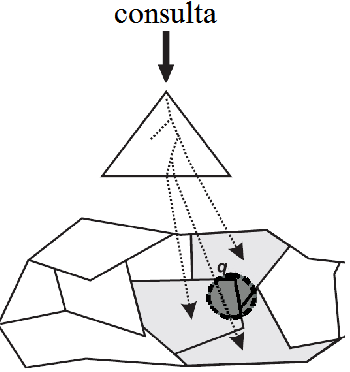
\includegraphics[width=0.32\columnwidth]{chapter2/candidate_regions.png}%\label{fig:slimbe:a}
    \label{fig:am_model}
    }
\subfigure[]
    {
    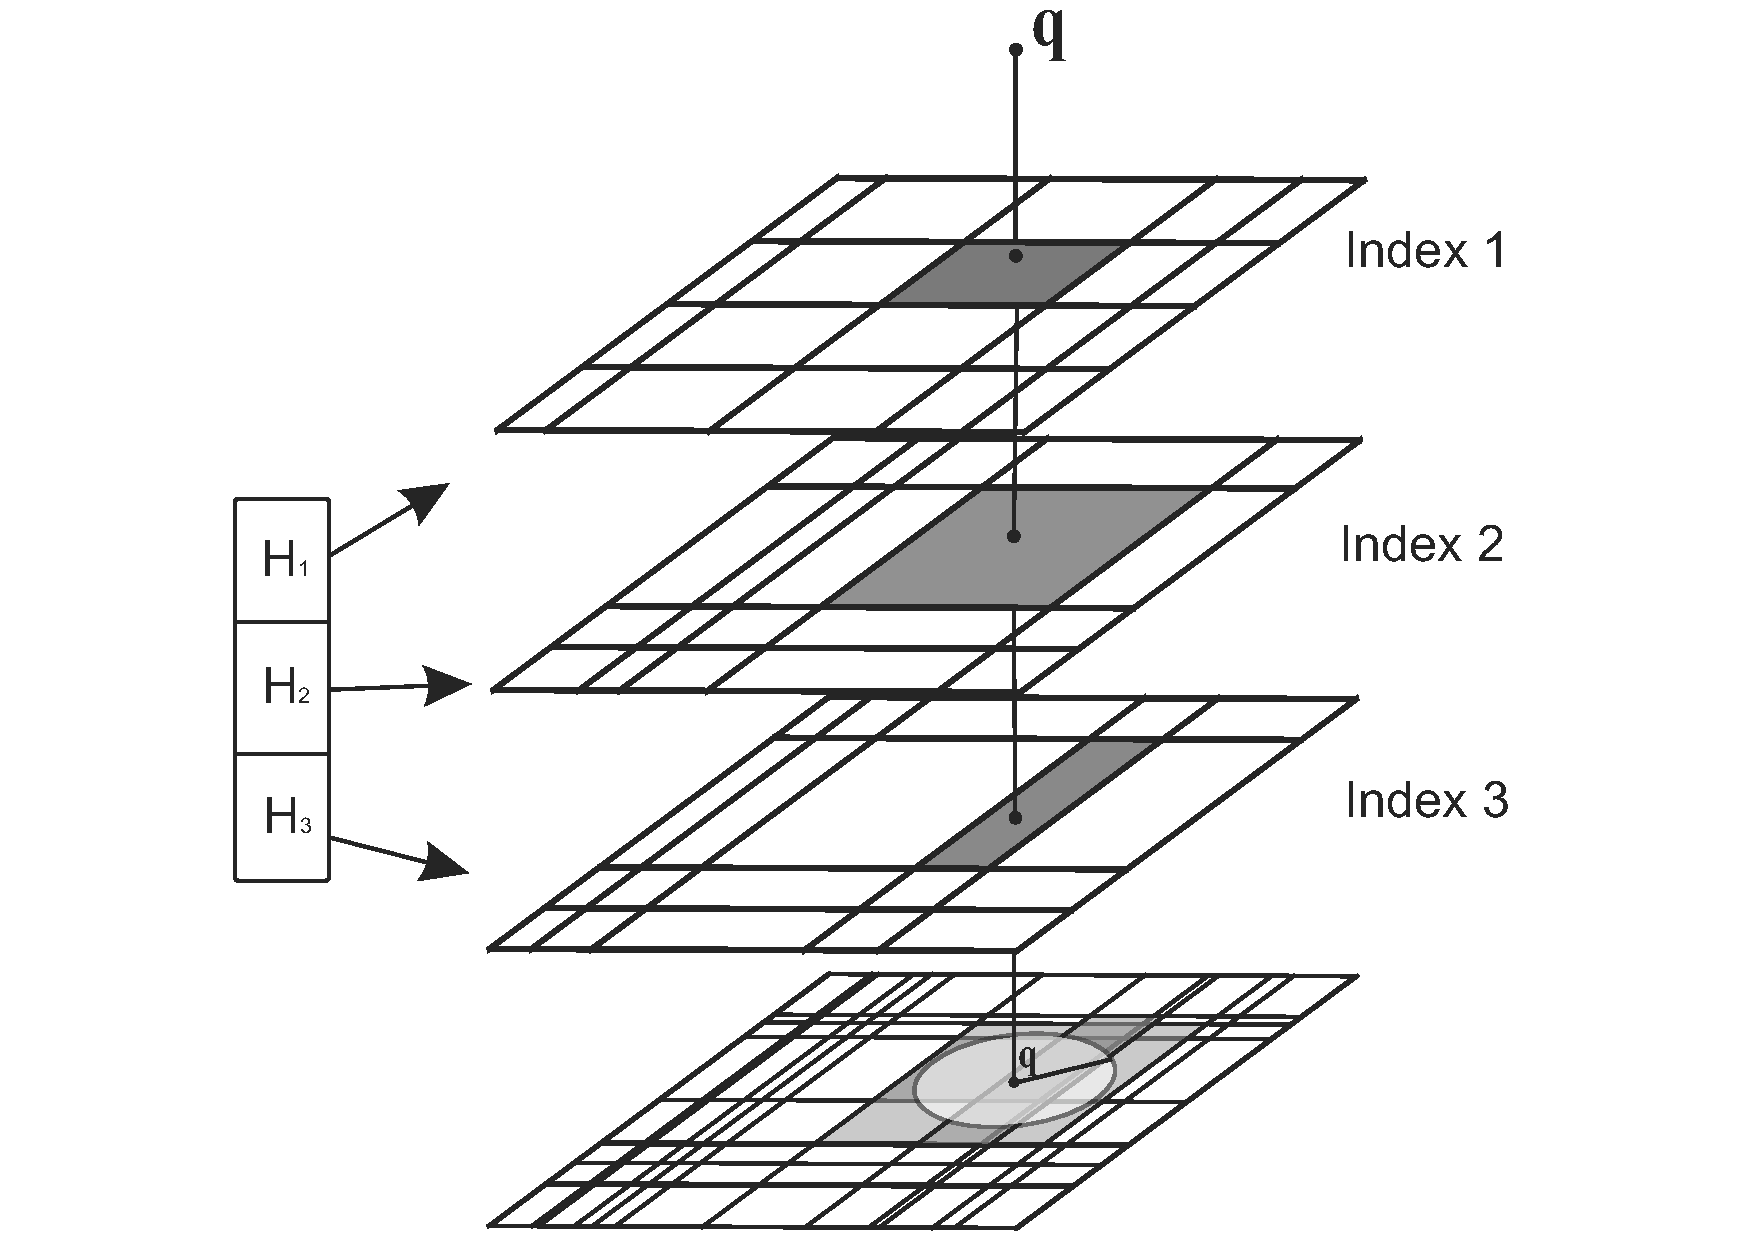
\includegraphics[width=0.37\columnwidth]{chapter2/lsh_basic_gray.pdf}%\label{fig:slimbe:a}
    \label{fig:lsh_model}
     }
\caption{Unificación del modelo de consulta por similitud. (a) Los Métodos de Acceso Métricos (MAMs). (b)  \textit{Locality Sensitive Hashing} (LSH).}
\label{fig:search_model}
\end{figure}


\section{Dominio de datos}

la concepción de un método de búsqueda debe considerar la naturaleza de los datos, a fin de explotar ciertas propiedades del espacio en donde están embebidos.

La gran mayoría de métodos de búsqueda supone que los datos pertenecen a un espacio n-dimensional. Esos espacios están en $R^n$, lo que permite el uso de propiedades geométricas en la solución. Por otro lado, algunos métodos tienen exigencias menos rigurosas, como el caso de los métodos basado en espacios métricos, que solo usan las distancias entre los puntos, y ninguna otra propiedad geométrica.


\subsection{Espacios Métricos}

Un espacio métrico es definido como  $\mathbb{M} = <S, d>$, donde $S$ es un universo de elementos y $d$ es una función de distancia (o métrica), definida sobre los elementos en $S$, que mide la disimilitud los objetos y satisfacen las siguientes condiciones, $\forall x, y, z \in S$:


\begin{tabular}{ l l }
  (1) $d(x, y) \geq 0   $ & positividad\\
  (2) $d(x, y) = 0 \leftrightarrow x = y$ & reflexibidad\\
  (3) $d(x, y) = d(y, x)$ & simetria\\
  (4) $d(x, y) \leq d(x, z) + d(y, z)$ & desigualdad triangular\\
\end{tabular}
\vspace{0.5cm}

La desigualdad triangular es considerado una de las propiedades mas importantes, pues es utilizada para establecer los límites del valor de distancia entre dos objetos sin la necesidad del cálculo real de distancia, acelerando así los algoritmos de consulta por similitud. Mas específicamente, dados los valores de distancia $d(x,z)$ y $d(y, z)$, los limites para el valor (desconocido) de $d(x, y)$ son $|d(x,z) - d(y, z)| \leq d(x, y) \leq d(x,z) + d(y, z)$.

No todas las propiedades (1)-(4) son necesarias para todos los métodos. Por ejemplo, se puede substituir (2) por una propiedad mas débil $\forall x \in S, d(x,x) = 0$, tornando el espacio pseudo-métrico. Los métodos que no obedecen las propiedades (3), (4) o ambas son típicamente llamados no métricos.


\subsection{Espacios Multidimensionales}

Si los objetos del dominio $S$ corresponden a los vectores de valores numéricos entonces el espacio es llamado Espacio Multidimensional o Espacio Vectorial con Dimensión Finita. Los objetos de un espacio multidimensional de dimensión $n$ (o $n$-dimensional) son representados por $n$ coordenadas de valores reales ${x_1, ..., x_n}$.

Las funciones de distancia métrica mas común para medir la similitud entre elementos en un Espacio Multidimensional son de la familia $L_p$, o Minkowski, definidas por:

\begin{equation}\label{lpnorm}
 L_p ((x_1,...,x_n), (y_1,...,y_n)) = (\sum_{i=1}^{n} |x_i - y_i|^p)^{1/p}
\end{equation}

\begin{itemize}

\item La distancia $L_1$ es también conocida como distancia \textbf{Manhattan}, y corresponde a una  simple suma de las diferencias absolutas de los componentes.

\item La distancia $L_2$ es también conocida como distancia \textbf{Euclidiana}, y corresponde a la idea usual de distancia en espacios $2D$ o $3D$.

\item La distancia $L_{\infty}$ es también conocida como \textbf{Chebychev}, y corresponde a la diferencia máxima absoluta entre los componentes, definida por:

\begin{equation}
   L_{\infty} ((x_1,...,x_n), (y_1,...,y_n)) = max_{i=1}^{n} |x_i - y_i|
\end{equation}

\end{itemize}

\begin{figure}[htp]
\centering
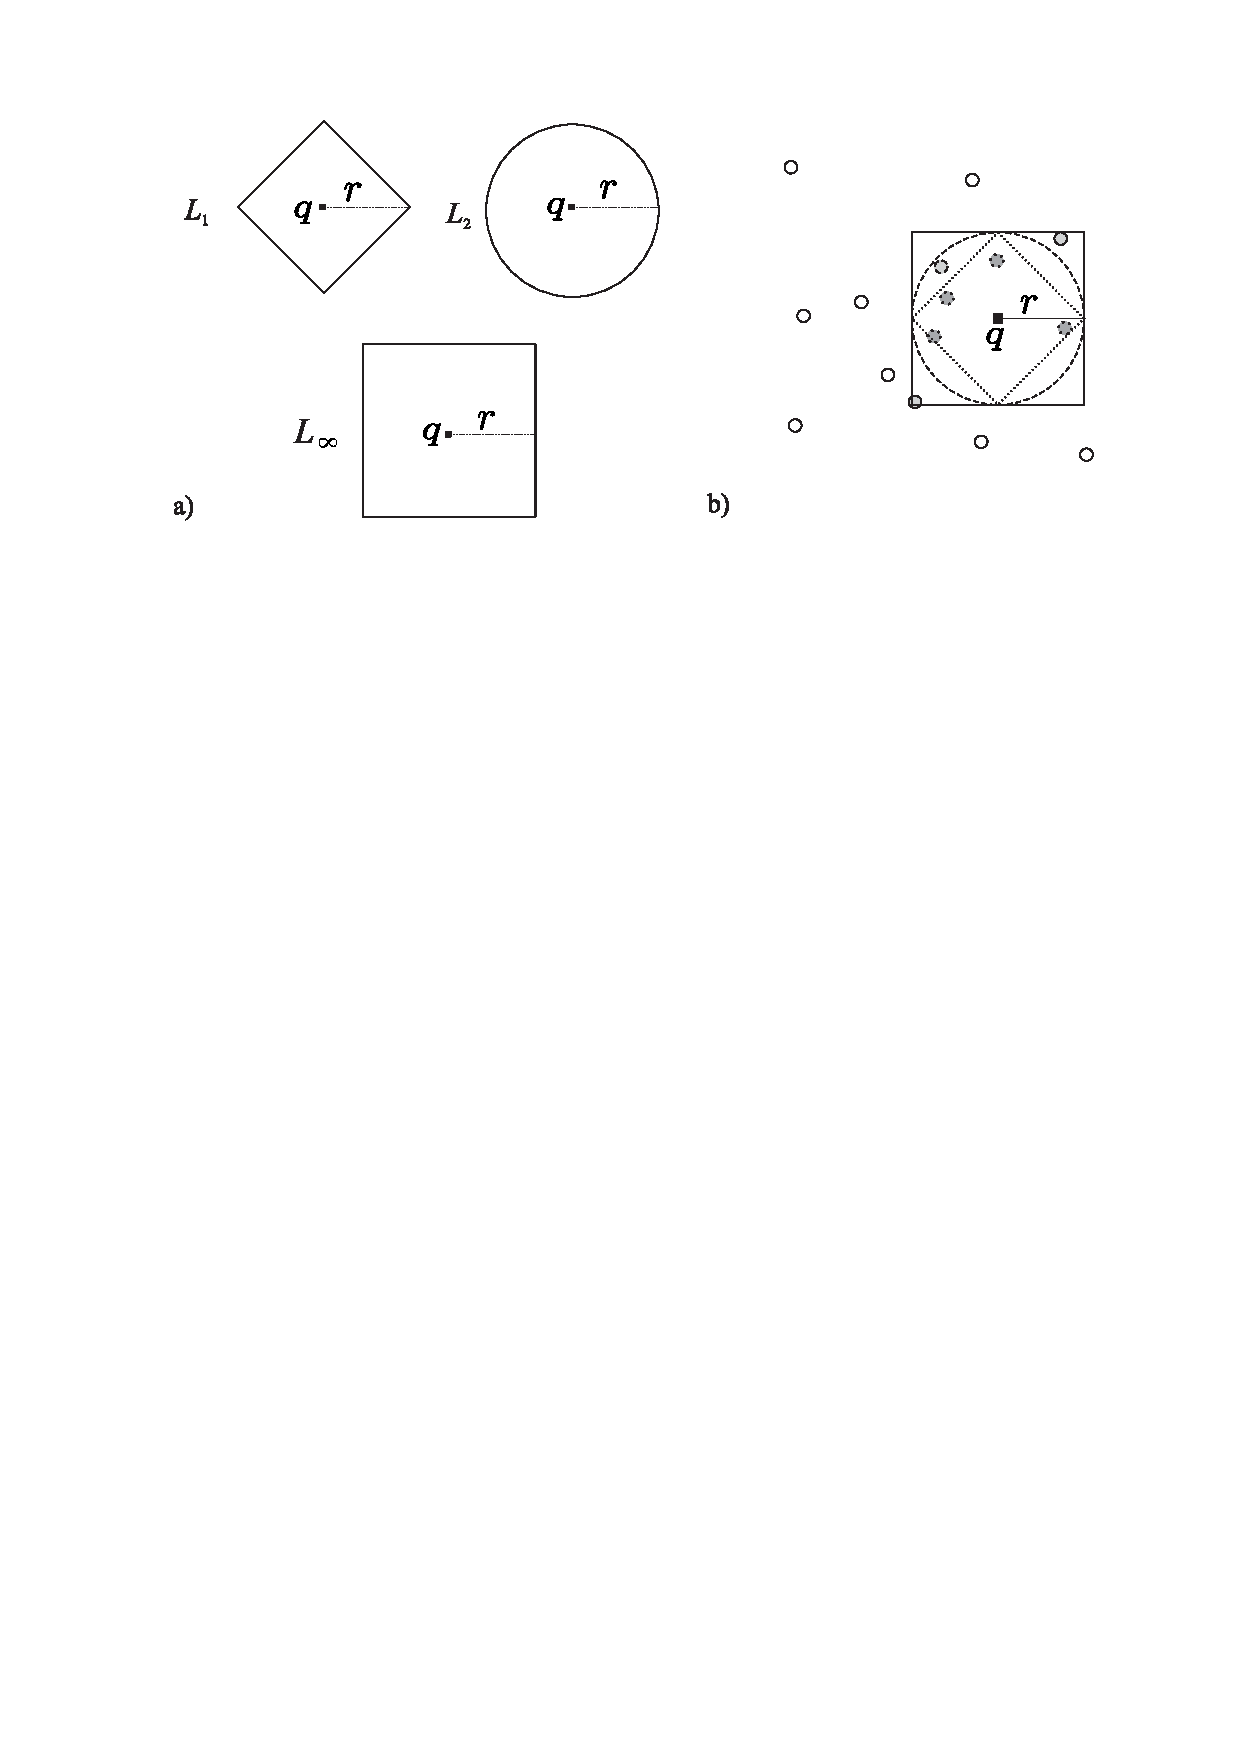
\includegraphics[width=0.9\columnwidth]{chapter2/lpnorms.pdf}
\caption{(a) Formas geométricas que ilustran la delimitación de una  región de búsqueda de acuerdo con la métrica $L_p$ utilizada. (b) Ejemplo de consulta por rango para diferentes métricas de la  familia $L_p$.}
\label{fig:lpnorms}
\end{figure}

La Figura \ref{fig:lpnorms}(a)  ilustra,  las distancias de la familia  $L_p$, el conjunto de puntos que están a la misma distancia $r$, a partir de un centro $q$, en un  espacio bi-dimensional.

La Figura \ref{fig:lpnorms}(b) representa un conjunto de objetos en un  espacio bi-dimensional, un objeto de consulta $q$, un radio de consulta $r$, los conjuntos de respuesta y tres métricas utilizadas: $L_1$, $L_2$ e $L_{\infty}$.

La \textbf{distancia de coseno} presentada en la Ecuación \ref{eq:2_3} es otra métrica de distancia popular para la búsqueda de $NN$ que ha demostrado ser particularmente eficaz para la recuperación de documentos \cite{Manning,Ravichandran}.

\begin{equation}\label{eq:2_3}
      d_{cosine}(X_i,X_j) = 1 - \frac{\sum\nolimits_{k=1}^{D} x_{ik} x_{jk}}{\sqrt{\sum\nolimits_{k=1}^{D} x_{ik}^2}\sqrt{\sum\nolimits_{k=1}^{D} x_{jk}^2}}
\end{equation}

También encontraremos la \textbf{distancia de Hamming} ampliamente en esta tesis, ya que es la métrica por defecto para comparar cadenas binarias (Ecuación \ref{eq:2_4})

\begin{equation}\label{eq:2_4}
     d_{hamming}(b_i,b_j) = \sum_{k=1}^{D} \delta[b_{ik} \neq b_{jk}]
\end{equation}

La función $\delta(.) = 1$ si su argumento es verdadero, y 0 en caso contrario. Por lo tanto, la distancia de Hamming cuenta el número de dimensiones correspondientes (bits) que no son iguales en los dos \textit{hashcodes}. \\

\section{Consultas por Similitud}\label{sec:consultas-similaridade}

Aplicaciones en la recuperación de información por similitud, por lo general crea un universo de objetos $\mathbb{U}$  y una función $d: \mathbb{U} \times \mathbb{U} \rightarrow \mathbf{R} $ que mide la distancia entre dos objetos en $\mathbb{U} $. En los espacios métricos, definimos $\mathbb{S} \subseteq \mathbb{U} $ como un conjunto finito de objetos, donde la función $d()$ mide la disimilitud entre objetos.

Dado un objeto de consulta $q \in \mathbb{U} $,  los objetos similares a $q$  se pueden recuperar de acuerdo a los siguientes tipos de consultas por similitud:

\paragraph{Consulta por radio (\textit{range query} Rq (q, r))} consulta que tiene como objetivo recuperar los objetos similares a $q$ que están dentro del rango de la consulta $r$.

\begin{equation}
    Rq(q, r) = \{ u \in S | d(u, q) \leq r \}
\end{equation}

En la Figura \ref{fig:rangeQuery} se representa una consulta por rango en un espacio bi-dimensional con la métrica $L_2$. Los elementos contenidos por el radio $e$ componen la respuesta. Vale recordad que no es necesario que el elemento de consulta pertenezca al conjunto de datos de búsqueda, debiendo este pertenecer al mismo dominio de datos.

\begin{figure}[htp]
\centering
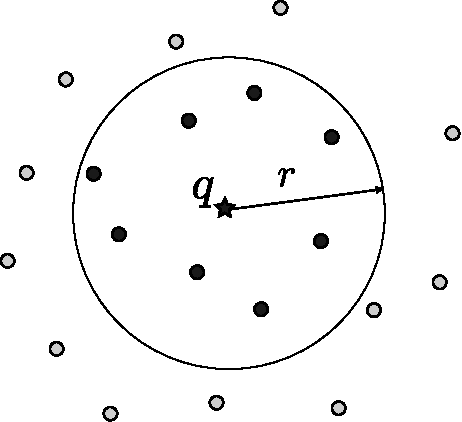
\includegraphics[width=0.3\columnwidth]{chapter2/range_query.pdf}
\caption{Ejemplo de consulta por rango.}
\label{fig:rangeQuery}
\end{figure}


\paragraph{Consulta de los k-vecinos más cercanos (\textit{k-Nearest neighbor query} - $kNN (q, k)$)} consulta que tiene como objetivo recuperar los $k$ objetos más cercanos al objeto de búsqueda $q$. O más formalmente, los $k$ vecinos más próximos definen el conjunto  $ C = \{s_1,s_2,...,s_k\} $ en que:

\begin{equation}
    \forall s_i \in C, \forall x_j \in S - C, d(q, s_i) \leq d(q, x_j)
\end{equation}

La Figura \ref{fig:knnQuery} ejemplifica una consulta kNN en un espacio bi-dimensional con la métrica $L_2$. En la figura, la consulta tiene como entrada el elemento de consulta $q$ y el valor de $k$ igual a $3$.  Los elementos conectados a $q$ corresponden al consulto de respuesta, considerando que en el ejemplo el elemento $q$ no pertenece al conjunto de datos.

\begin{figure}[htp]
\centering
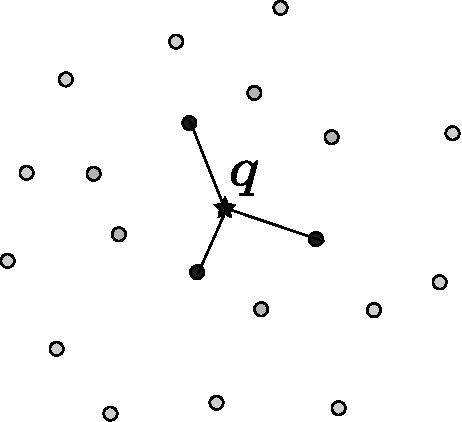
\includegraphics[width=0.28\columnwidth]{chapter2/knn_query.pdf}
\caption{Ejemplo  de consulta de los k-vecinos más cercanos.}
\label{fig:knnQuery}
\end{figure}
 

\paragraph{Consulta por rango aproximada - $(1 + \varepsilon)  Rq(q, r)$}

Consulta que busca recuperar los objetos cercanos a $q$ que se encuentran dentro del radio de consulta  $(1 + \varepsilon) \times r$. O, más formalmente:

\begin{equation}
    (1 + \varepsilon) Rq(q, r) = \{ u \in S | d(u, q) \leq (1 + \varepsilon) \times r \}
\end{equation}

La Figura \ref{fig:AproximateRangeQuery} ejemplifica una consulta de este tipo para $L_2$. Los elementos dentro del radio de consulta  $(1 + \varepsilon)\times r$ componen la respuesta aproximada.
\begin{figure}[htp]
\centering
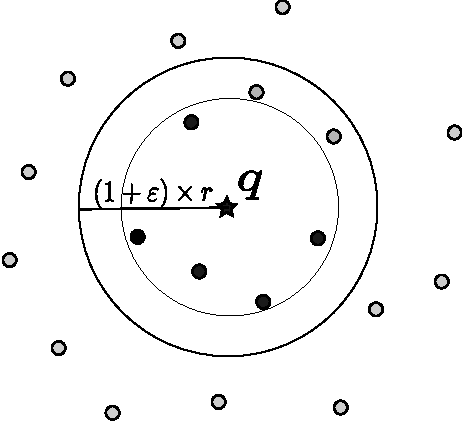
\includegraphics[width=0.32\columnwidth]{chapter2/app-range_query.pdf}
\caption{Ejemplo de consulta  por  rango aproximada.}
\label{fig:AproximateRangeQuery}
\end{figure}
%@ refazer figura


\paragraph{Consulta Aproximada a los $k$-vecinos más cercanos  - $(1 + \varepsilon) - kNN(q, k)$}
Sea $r$ la distancia entre el objeto de consulta $q$ y el elemento más distante entre los $k$ verdaderos vecinos más próximos, esto es,

\begin{equation}
r = max\{ s_j \in S | d(q, s_j)\}
\end{equation}

La búsqueda $(1 + \varepsilon)-kNN$  para los $k$ elementos  mas similares a $q$ consiste en encontrar un conjunto $C' = \{s_1', s_2', ..., s_k'\}$ en donde,

\begin{equation}
\forall s_i' \in C', d(q, s_i') \leq (1 + \varepsilon) \times r
\end{equation}

El factor $(1 + \varepsilon)$  es usualmente llamado  \textbf{factor de aproximación}, y indica que el conjunto de la solución $C'$ está dentro de un \textbf{error relativo}  $\varepsilon$  a la respuesta exacta.  Ver Figura \ref{fig:nearbyKnnQuery}.
\begin{figure}[htp]
\centering
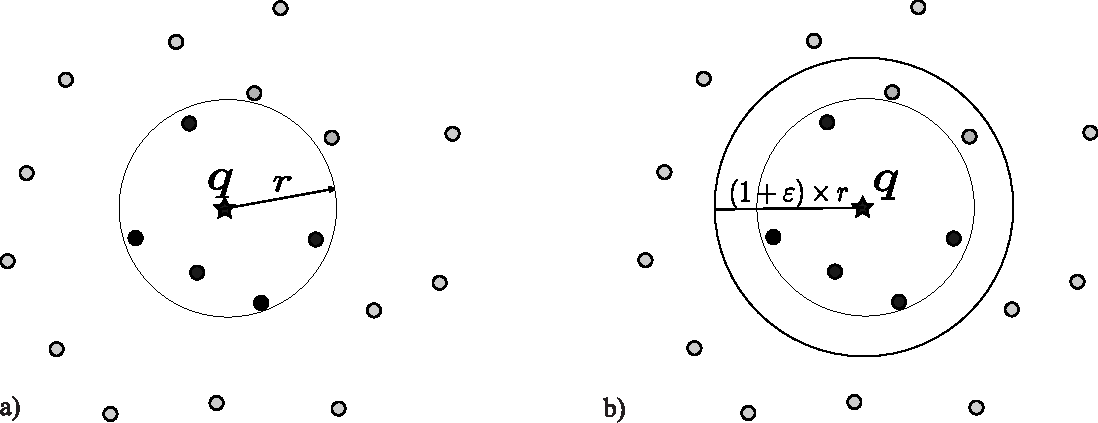
\includegraphics[width=0.85\columnwidth]{chapter2/nearby_knn_query.pdf}
\caption{Búsqueda aproximada 5-NN. (a) busca exacta. (b) busca aproximada.  }
\label{fig:nearbyKnnQuery}
\end{figure}

 

\section{La Maldición  de la alta Dimensionalidad} \label{sec:madicao-dimensionalidade}

La eficiencia de los métodos de búsqueda por similitud dependen mucho de la dimensionalidad. Aunque el tiempo de búsqueda pueda alcanzar un costo logarítmico en relación al tamaño de los datos, este va crecer exponencialmente con la dimensionalidad de los datos.

Para dimensiones moderadas, la mayoría de los métodos ejecutas las consultas de manera suficientemente eficientes para permitir una solución exacta  en un tiempo razonable. Para dimensiones más altas, se vuelve viable el uso de métodos aproximados,  lo que implica en un \textit{trade-off}  entre la precisión y la eficiencia. Para dimensiones más altas ese \textit{trade-off}  va convertirse progresivamente más relevante, resultando en penalidades mayores en términos de precisión, a fin de obtener una eficiencia aceptable.

El problemas de ``la maldición de la alta dimensionalidad'' fue estudiado originalmente por Bellman \cite{citeulike:Bellman}, observando que particiones del espacio de soluciones en problemas de optimización son ineficientes en problema con datos en altas dimensiones. Los efectos de ``maldición'' en Métodos de Acceso Espaciales (MAEs) y Métodos de Acceso Métricos (MAMs) son discutidos en  \cite{aleman_high_dimensional, WhatsWrong, DBLP:journals/corr/abs-0906-0391}.

%\section{Soluciones Aproximadas}\label{sec:solucoes-aproximadas}
\section{Búsqueda aproximada  de los vecinos más cercanos (ANN)}

En esta sección   definimos formalmente el problema de la búsqueda del vecino más cercano (Nearest Neighbor search - NN). Se examinará entonces la versión simplificada de la búsqueda NN conocida como búsqueda NN aproximada, el campo en el que se basa esta tesis, y describirá cómo difiere de los algoritmos alternativos para resolver el problema de búsqueda NN.

Los trabajos descritos en este capitulo todos comparten la definición del mismo problema. Dado un conjunto de datos X que consiste de N puntos ($X \in R ^ {NxD} = [x_1, x_2,..., x_N]^T$), donde cada punto $x_i \in R^D$ es un vector D-dimensional de valores reales (vector característica). El objetivo es construir un conjunto de $m$ funciones hash $\{ h_m : R^D \rightarrow {0, 1}\}_{m=1}^K$ cuya salida puede ser concatenada como [$h_1(x_i), h_2(x_i), ..., h_\Nhashfunctions(x_i)$]  el cual cumple la función de codificar el vector característica.  Para codificar se necesitan funciones \textit{hash} que preserven la similitud del espacio original.  
 
La búsqueda de vecinos más cercanos se puede definir como el problema de recuperar el punto de datos más cercano $ NN(q) $ para una consulta $ q \in R^D$ en un conjunto de datos de $N$ puntos  $ [x_1. x_2 , ..., x_N]^T $ donde $x_i \in R^D$. La similitud entre los puntos   se define por una función de distancia  $\{ d(.,.) : R^D \times R^D  \}$.   Es fácil generalizar esta definición de problema para devolver los vecinos $K$ más cercanos a la consulta. Esta variante se conoce   como búsqueda k-NN y es un componente fundamental en una amplia gama de diferentes métodos de aprendizaje de máquinas. La función de distancia $d(x,y)$ entre los puntos de datos se suele calcular utilizando una métrica de distancia genérica como la $l_p - norm$ (Ecuación \ref{lpnorm}).

Para buscar $NNs$ a una consulta necesitamos construir una estructura de datos o algoritmo que tome nuestra noción seleccionada de distancia y recupera los puntos de datos que están cerca de la consulta bajo esa métrica de distancia específica. La búsqueda por fuerza bruta es un algoritmo sencillo para resolver el problema de búsqueda del vecino más cercano con cualquier métrica de distancia deseada. En la búsqueda por fuerza bruta se calcula la distancia a todos los puntos en la base de datos y los puntos  con la menor distancia a la consulta son devueltos como el vecino más cercano. Las ventajas de la búsqueda de la fuerza bruta son su simplicidad de la puesta en práctica y su garantía que los vecinos más cercanos   serán recuperados eventualmente. Sin embargo, comparar exhaustivamente la consulta con cada punto en la base de datos da una complejidad temporal $O (ND)$ que hace rápidamente la búsqueda de fuerza bruta intratable para la búsqueda de vecinos más cercanos a través de conjuntos de datos con muchos puntos de datos (N) y una dimensionalidad moderada a alta (RE). En esta situación, se requiere un enfoque más informado del problema de búsqueda del vecino más cercano.\\
 
En la  sección \ref{sec:lsh}, introduciremos el método \textit{Locality Sensitive Hashing (LSH)}, una familiar de algoritmos que proveen un método para resolver búsqueda aproximada de los vecinos mas próximos con un tiempo de consulta constante. 

\subsection{\textit{Locality Sensitive Hashing}}\label{sec:lsh}

Algunos trabajos de búsqueda aproximada  \cite{lsh_hamming,lsh,hashing_algoritghms_survey} exploran la idea de mapear los objetos de un conjunto de datos y agruparlos en  \textit{buckets} con el objetivo de ejecutar consultas por similitud aproximada dentro de los  \textit{buckets} asociados al objeto de consulta. En particular, el método \textit{Locality Sensitive Hashing} (LSH) fue ideado para resolver eficientemente consultas por rango aproximada $((1+\epsilon) Rq(q, r))$. Como fue definido en la Sección  \ref{sec:consultas-similaridade}, este tipo de consulta busca recuperar los objetos que se encuentran dentro de un radio de consulta $(1+\epsilon) \times r$. La idea principal es que, si dos objetos son próximos en el espacio original, esos dos objetos tienden a permanecer próximos después de una operación de proyección escalar randomica. Así, dada una función \textit{hash} $h(x)$ que mapea un objeto ($x$) de dimensión $n$ a un valor unidimensional, la función es sensible a la localidad si la posibilidad de mapeamiento de dos objetos $x_1$, $x_2$ al mismo valor crece a la medida que la distancia  $d(x_1, x_2)$  disminuye. Formalmente:

\paragraph{Definición} Dado un valor de distancia $r$, un factor de aproximación $1+\epsilon$, las probabilidades $P_1$ y $P_2$, tal que $P_1 > P_2$, la función \textit{hash}  $h()$ es sensible a la localidad de los datos si satisface las siguientes condiciones:

\begin{itemize}
\item $Se \ d(x_1, x_2) \leq r \Rightarrow Pr[h(x_1) = h(x_2)]  \geq P_1$.

Esto quiere decir que para dos objetos  $x_1$ y $x_2$ en $R^n$  que están lo suficientemente próximos,  hay una probabilidad   $P_1$ que ellos caigan en el mismo \textit{bucket}.

\item $Se\ d(x_1, x_2) > (1+\epsilon) \times r  \Rightarrow Pr[h(x_1) = h(x_2)] \leq P_2$.

Esto quiere decir que para dos objetos $x_1$ y $x_2$ en $R^n$ que están distantes, hay una probabilidad $P_2 < P_1$ que ellos caigan en el mismo  \textit{bucket}.

\end{itemize}

El esquema propuesto en \cite{lsh} fue proyectado para trabajar con distribuciones p-estables de la siguiente manera: calcular el producto escalar $\vec{a} \cdot \vec{x}$ para atribuir un valor \textit{hash} para cada vector $x$. La función  \textit{hash} precisa de valores randomicos $\vec{a}$ y $b$, en que $\vec{a}$ es un vector n-dimensional con valores independientemente escogidos a partir de distribuciones p-estables (Cauchy o Gaussiana) y $b$ es un número real escogido dentro de un intervalo $[0,\omega]$. Por tanto la función \textit{hash} $h(x)$ esta dada por:


\begin{equation}\label{eq:lsh}
    h(x) = \lfloor\frac{\vec{a} \cdot \vec{x} + b}{ \omega }\rfloor
\end{equation}

La ecuación \ref{eq:lsh} tiene una interpretación simple. Considere la Figura \ref{fig:quantization}: $\vec{p_1}$ y $\vec{p_2}$ son dos vectores en $\mathbf{R}^2$, $\vec{a}$ es un vector normal unitario e $b$ es un número randomico real. A inclinación de la recta pasando por el origen coincide con la dirección de $\vec{a}$. Así, $\vec{p_1}$  es proyectado sobre la línea $\vec{a}$  calculando el producto escalar  $\vec{a} \cdot \vec{p_1}$. Esa proyección es cuantizada en intervalos de tamaño fijo  $\omega$, definiendo el punto A. El mismo procedimiento es repetido para $\vec{p_2}$, definido el punto B.

\begin{figure}[htp]\centering
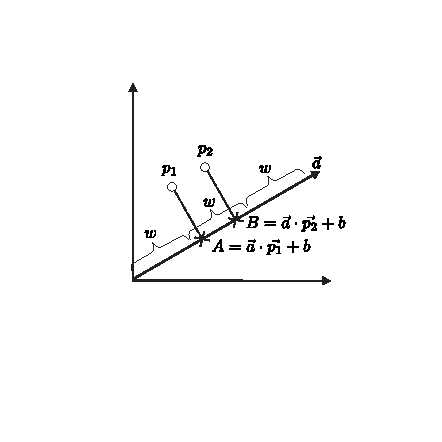
\includegraphics[width=0.35\columnwidth]{chapter2/lsh_projection.pdf}
\caption{Interpretación geométrica de proyección de los  vectores $\vec{p_1}$ y $\vec{p_2}$ en LSH.}
\label{fig:quantization}
\end{figure}

Para amplia a diferencia entra las probabilidades $P_1$ y $P_2$ se puede usar $\Nhashfunctions$ funciones \textit{hash} diferentes. Esto aumenta las probabilidades dado que \mbox{$(P_1/P_2)^\Nhashfunctions > P_1/P_2$}, asegurando así que si dos objetos están muy distantes, la probabilidad de que caigan en el mismo \textit{bucket} sea baja. Sin embargo, aunque sea importante evitar que objetos distantes caigan en el mismo \textit{bucket} para preservar la proximidad espacial, esto no es una condición suficiente. Es igualmente importante asegurar que objetos próximos en el espacio original tengan una alta probabilidad que aparecer en el mismo \textit{bucket}. Así, como eso no puede ser alcanzado usando solo una estructura \textit{hash}, LSH resuelve ese problema considerando $L$ proyecciones independientes, ósea, la construcción de $L$ tablas \textit{hash} ($L$ subíndices) \cite{lshtutorial,taoLSBLSH}.

Así usando colecciones diferentes de $\Nhashfunctions$ funciones \textit{hash} $H = \{h_1, h_2, ..., h_\Nhashfunctions\}$, siendo una colección cada sub-indice, cada objeto $x$ de un conjunto de datos es mapeado en \textit{buckets}, efectivamente particionando el conjunto de datos en varios grupos pequeños (los \textit{buckets}) para cada uno de los $L$ subindices. La estructura de datos será entonces formada por $L$ subíndices. LSH divide el espacio de búsqueda empleando $\Nhashfunctions$ funciones \textit{hash} escogidas aleatoriamente de una distribución Gaussiana (o Cauchy). Un número de funciones \textit{hash} $\Nhashfunctions$ determina cuan esparzo o denso será el espacio de búsqueda. Al aumentar el valor de $\Nhashfunctions$, los objetos tiendes a ser distribuidos en \textit{buckets} de manera bastante uniforme, reduciendo la precisión de las consultas ya que es más probable que objetos similares caigan en \textit{buckets} diferentes. Para atenuar ese efecto negativo, son necesarias muchas tablas \textit{hash}. Por otro lado, al disminuir el valor de $\Nhashfunctions$, el número de colisiones aumenta, así como el número de elemento a ser tratados en tiempo de consulta. Así, el desempeño de las consultas disminuye.

El proceso de indexación de un conjunto de datos $S$ usando LSH es mostrado en el Algoritmo \ref{alg:lshalgorithm}. Cada elemento $x$ del conjunto de elementos $S$ es proyectado usando   $\Nhashfunctions$  funciones \textit{hash} que transforma el elemeno $x$ en $\Nhashfunctions$  números reales ($x'$, el vector \textit{hash}). Esos $\Nhashfunctions$  números son entonces cuantificados con un único número ($g$).
 \begin{lstlisting}[mathescape, frame=single, label=alg:lshalgorithm,caption=Algoritmo de construcción para LSH]
Input: El conjunto de dados  $S$
Output: Todos los objetos mapeados en las $L$ tablas $hash$
  for $i = 1$ to $L$ do
    $H_{i} \Leftarrow \{h_1,...,h_\Nhashfunctions\}$       //Inicializar tabla $T_i$ con un conjunto de funciones $hash$ $H_i$
  end for
  for $i = 1$ to $L$  do
    foreach $x$ en $S$ do
      $x' \Leftarrow $ $<h_1(x),...,h_\Nhashfunctions(x) >$  //Proyectar $x$:  $\Nhashfunctions$ veces usando el conjunto de funciones $hash$ $H_{i}$
      $g \Leftarrow quantize(x')$                            // Calcular el valor $hash$ final
      $I \Leftarrow T_i[\  g $ mod $ | T_{i} |\ ]$     //localizar el $bucket$ $I$
      Insertar la entrada $<x, g>$  en $I$, almacenando la referencia de $x$ y el valor $g$
    end for
  end for
\end{lstlisting}


Una vez que cada \textit{bucket} es definido en términos de similitud (esto es, elementos semejantes tienden a ser encontrados en el mismo \textit{bucket}, es probable encontrar los vecinos más próximos a un objeto $q$ en los \textit{buckets} recuperados por cada conjunto de funciones \textit{hash}). Así, en vez de hacer comparaciones para reducir el espacio de búsqueda, LSH mapea directamente los objetos a los \textit{buckets}. Luego, es posible obtener un costo sub-linear en las consultas. En una consulta kNN, a fin de retornar los $k$ vecinos más próximos, apenas las distancias entre $q$ y los elementos dentro de los \textit{buckets} son calculados. En una consulta por rango sucede lo mismo, mas la condición de consulta es diferente y solo los elementos dentro del radio de consulta son retornados. El algoritmo de consulta por rango aproximada es descrito en el Algoritmo  \ref{alg:lsh_rq}.

\begin{lstlisting}[mathescape, frame=single, label=alg:lsh_rq,caption=Consulta por rango aproximada usando LSH]
Input: El objeto de consulta $q$ y el radio de consulta $r$
Output:  Los objetos que satisfacen las condiciones de consulta.
  for $i = 1$ to $L$  do
    $q' \Leftarrow $ $<h_1(q),...,h_\Nhashfunctions(q)>$ //Proyectar $x$:  $\Nhashfunctions$ veces usando el conjunto de funciones hash $H_{i}$
    $g \Leftarrow quantize(q')$   //  calcular el valor hash final
    $I \Leftarrow T_{i}[\  g $ mod $ | T_{i} |\ ]$   //localizar el bucket $I$
    foreach $e$ en $I$ do
      if $e.g = g  \wedge  d(q, e.x) \leq r $ then
        retornar $e.x$ si no fue reportado
      end if
    end for
  end for
\end{lstlisting}

El algoritmo kNN puede ser obtenido por medio de simples modificaciones en el Algoritmo \ref{alg:lsh_rq}. Básicamente, el algoritmo kNN terminará cuando se encuentre $k$ objetos distintos o si no hubiere más \textit{buckets} para explorar. No obstante, es importante recordar que LSH garantiza resultados de calidad previsible apenas para consultas por rango aproximada $((1+\epsilon)-Rq(q, r))$. Además, algunos inconvenientes de LSH no fueron resueltos por completo, por ejemplo: (1) LSH requiere varios sub índices de moco que cada subíndice organiza el conjunto de datos entero usando una tabla \textit{hash} con funciones \textit{hash} independientes. Esa exigencia es extremadamente crítica para mejorar la precisión de búsqueda, mas lleva a un alto consumo de memoria; (2) LSH tiene una dependencia crítica de los parámetros de dominio, que determina el número de funciones \textit{hash} y el número de tablas \textit{hash}.


 En \textit{hash} los autores propusieron LSH Multi-probe, que busca mantener un costo de memoria aceptable. LSH Multi-prove está basado en el LSH clásico, mas en cuanto el algoritmo de consulta LSH examina apenas un \textit{bucket} para cada tabla \textit{hash}, LSH Muli-probe examina los \textit{buckets} que son susceptibles de contener los resultados de consulta por cada tabla \textit{hash}. Consecuentemente, el número de tablas \textit{hash} es reducido sin perdida significativa de precisión. Intuitivamente esta propuesta verifica los \textit{buckets} de forma más inteligente, generando $\tau$ $probes$ por cada tabla   \textit{hash}, lo que permite explorar $\tau$ \textit{buckets} por sub-índice, y como consecuencia, aumentar el número de candidatos sin incrementar el número de subíndices.

Una investigación más reciente sobre el método LSH \cite{modelinglsh}  muestra que el desempeño en las consultas no solo dependen de la distribución general del conjunto de datos, mas también de la distribución local en torno a un objeto de consulta. En el método LSH Multi-probe, un número fijo de $probes$ puede ser insuficiente para algunas consultas y mayor del que es necesario para otras. No obstante aun es complicado ajustar el número de funciones \textit{hash} asociado al radio de consulta.

Dado que los parámetros también dependen del número de objetos a ser indexados, el método LSH no es una solución incremental. Para lidiar con este problema, una nueva propuesta fui presentado, el método LSH-Forest \cite{lshforest}. Esa técnica fue desarrollada para soportar auto-ajuste en relación al número de funciones \textit{hash}. Esencialmente, el método LSH-Forest es una colección de arboles de prefijos donde cada una puede tener un número diferente de funciones \textit{hash}. No obstante, aun es necesario ajustar el número de subíndices, o sea, el número de arboles prefijo. Además, no esta claro su desempeño en sistemas que trabajan con datos distorsionados, en donde se tiende a verificar más candidatos del que es necesario en pequeñas áreas densas y tener candidatos insuficientes para los puntos de consulta en áreas esparzas.


En ese mismo escenario,  la técnica LSH Multi-level \cite{DBLP:journals/jidm/OcsaS10}, desarrollada en el contexto de este trabajo, propone un nuevo esquema de \textit{hashing} para resolver algunos de esos problemas. Especificamente, utilizan un esquema multiresolución para resolver la dependencia de parámetros de dominio. El método no espera los parámetros del dominio de datos, pues, se adapta dinámicamente durante el proceso de indexación, gracias a las habilidades auto-adaptativas de la estructura del índice multi-nivel. Este método presenta un mejor desempeño en termino de tiempo y espacio comparado con otras propuestas \textit{hash}, pues la técnica multi-nivel distribuir los objeto en \textit{buckets} de manera uniforme en todos los niveles. Esto porque, en contraste con LSH, el método LSH Multi-level usa la estructura multi-resolución para calcular y localizar los vectores \textit{hash} apropiados para una consulta especifica. Así, varios vectores \textit{hash} de diferentes resoluciones son calculados por cada índice en el proceso de consulta y, como consecuencia, no se precisa de mas índices para garantizar resultados de la misma calidad.

Recientemente, en \cite{taoLSBLSH}  los autores propusieron el método LSB-Forest. Este trabajo mejor la técnica LSH-Forest, y a fin de garantizar la calidad y eficiencia de recuperación de datos multidimensionales, utiliza representaciones basadas en \textit{space-filling curves} y arboles B. De ese modo, los valores \textit{hash} son representado como valores unidimensionales usando tanto la proyección LSH como las curvas Z. Además, varios arboles B son usados para indexas los datos con el objetivo de mejorar la calidad de los resultados. Una desventaja de los arboles LSB es que usa lecturas/escrituras randomicas, lo que conlleva requiere un número considerable de accesos a disco cuando el conjunto de datos es grande. Para resolver ese problema, el método HashFile \cite{lshHashFile}  fue propuesto. Como será detallado en la siguiente sección, en comparación a los métodos actuales LSH, el método HashFile solo divide recursivamente los \textit{buckets} densos para alcanzar particiones mas equilibradas. Cada \textit{bucket} almacena un número fijo de objetos, mas el método aprovecha la lectura secuencial en vez de usar el acceso randomico, como es el caso en los arboles  B. Este método esta basado en conceptos de proyección aleatoria (\textit{Random Projection}).
 
 

\subsection{LSH con Projección Aleatória}\label{sec:hashfile}

%In this dissertation I will be primarily interested in the locality sensitive hash function
%family for the inner product similarity which traditionally has been used as a baseline
%for comparison by existing research in the learning to hash literature. The inner product
%similarity is defined in Equation 2.6.


%LSH puede ser usado también con familia de funciones \textit{hash} para buscar la similitud usando producto punto el cual ha sido tradicionalmente usado como base de comparación en varias investigaciones. El producto punto es definido como:  

%\begin{equation}\label{eq:dotproduct}
%d(p, q) =   \Sigma_{i=1}^d h_i \cdot o_i \\
%                =  p^T q
%\end{equation}

%La ecuación \ref{eq:dotproduct} puede ser interpretado como la medida de similitud coseno entre dos vector unitarios   normalizados. La medida de similitud  coseno mide la cercanía entre dos puntos que están en un ángulo $\tetha$.
El algoritmo de proyección aleatoria (Random Projection) básicamente usa vectores aleatorios provenientes de una distribución estable. El algoritmo es robusto contra el ruido y utiliza un enfoque probabilístico, consiguiendo reducir significativamente el costo computacional de la búsqueda con una pequeña perdida de precisión. La naturaleza aleatoria de la técnica permite una comparación eficiente de secuencias muy largas para el descubrimiento de características relevantes.

Un caso de esta familia de funciones que usan protección aleatoria  es  el  método HashFile \cite{lshHashFile}  fue propuesto para responder consultas kNN exactas en el espacio $L_1$  y $L_2$. El método combina las ventajas de la proyección aleatoria  y la  lectura secuencial. 

%Al contrario de otros métodos basado en LSH, en donde cada  \textit{bucket} es asociado a una concatenación de $m$ valores \textit{hash}, este método particiona recursivamente  los \textit{buckets}  densos que son organizados en un estructura jerárquica. Note que al contrario de  la mayoría  de los métodos LSH, este método solo necesita de un sub-indice para garantizar resultados de calidad. De ese modo, dado un objeto de consulta $q$, el algoritmo de búsqueda solo explorar los \textit{buckets} que están cerca al objeto de consulta usando el esquema de búsqueda $\textit{top-down}$. Los \textit{top-down}. Los\textit{buckets}   candidatos en cada nodo son almacenados secuencialmente  en orden creciente  a su valor \textit{hash}  y  pueden ser eficientemente  cargados a memoria principal. Los resultados muestran que este método supera métodos recientes, que representan el estado del arte en métodos de indexación, para consultas kNN exactas y aproximadas.

\subsubsection{Projección Aleatória}

La proyección aleatoria es un método de reducción de la dimensionalidad de los datos que es computacionalmente eficiente y suficientemente preciso. Dado un conjunto de datos $S$ con $N$ puntos de dimensión $n$ y una matriz aleatoria  $ R_{n \times k} $, la proyección es calculada de la siguiente manera.

\begin{equation}
S'_{N \times k} = S_{N \times n} \times R _{n \times k}
\end{equation}

La proyección resulta en un conjunto de datos  $S'$ k-dimensional con $N$ puntos. La proyección aleatoria puede preservar la distancia $L_1$ o $L_2$ en un espacio reducido, lo que es especificado por el Lema Jonhson-Lindenstrauss.


\paragraph*{Lema de Jonhson-Lindenstrauss:} Dado $\epsilon > 0$ es un numero  $N$, sea $k$ un  entero positivo tal que $k \geq k_0 = O (\epsilon^{-2}log N)$. Para cada conjunto $S$ de $N$ puntos en  $\mathbb{R}^n$, existe $f: \mathbb{R}^n \rightarrow  \mathbb{R}^k$   tal que para todo $u,v \in S$, se tiene:

\begin{equation}\label{eq:JL-lemma}
  (1 - \epsilon) \parallel u - v \parallel^2 \leq \parallel f(u) - f(v) \parallel^2 \leq (1 + \epsilon)\parallel u - v \parallel^2
\end{equation}

%En los últimos años, el Lema de Jonhson-Lindenstrauss (JL) ha sido útil en la resolución de una variedad de problemas. La idea es la siguiente: al obtener una baja representación dimensional de los datos, JL acelera cierto algoritmo de forma significativa, en especial los algoritmos cuyo tiempo de ejecución dependen exponencialmente de la dimensión del espacio de trabajo (hay una serie de problemas prácticos para los cuales los algoritmos más conocidos tienen ese comportamiento). Al mismo tiempo, JL provee una garantía de conservación de la proximidad después de una operación de proyección sobre cada par de distancias y generalmente es suficiente para establecer que la solución encontrada en el espacio reducido es una buena aproximación de la solución óptima en el espacio original.

Algunos ejemplos de aplicación fueron presentado en \cite{Indyk:1998:ANN:276698.276876}. Por ejemplo, Indyk y Motwani mostraron que el Lema JL es útil para resolver el problema de búsqueda aproximada al vecino más cercano, donde después de algunos procedimiento de pre-procesamiento del conjunto de datos, consultas de este tipo son respondidas: Dado un punto arbitrario $x$ y un punto $y \in P$, para cada punto $z \in P$ se satisface $ \|x - z\| \geq (1 - \epsilon)\|x - y\|$.

\subsubsection{Restricción de la distancia para consultas kNN usando $L_1$}

Supongo que  $\mathcal{H}$  es una función \textit{hash}  derivada de  $R_{n \times k}$   tal que esta mapea un objeto $o$
 de dimensión $n$ en un valor unidimensional.

\begin{equation}\label{eq:hashfile}
\mathcal{H}(o) = \lfloor \Sigma_{i=1}^n h_i \cdot o_i \rfloor
\end{equation}

Dado que cada elemento $h_i$  está dentro de $\mathcal{H}$  para valores randomicos $\{-1,0,1\}$,  se puede   fácilmente  alcanzar un \textit{lower bound} para consultas con la  distancia $L_1$.

\paragraph*{Limite Inferior para $L_1$} Dado dos puntos $x$ y $y$ de dimensión $n$, y una función  \textit{hash} $\mathcal{H} : \mathbb{R}^n \rightarrow \mathbb{R}^1$ con  $h_i \in \{-1,0,1\}$, se tiene.

\begin{equation}\label{eq:LBL1}
 \parallel x - y \parallel_{L_1} \geq | \mathcal{H}(x) - \mathcal{H}(y) | - 1
\end{equation}

Así, una proyección aleatoria puede ser usada para particionar un gran volumen de datos en \textit{buckets}, en un espacio unidimensional. Las páginas en disco pueden ser almacenados secuencialmente en orden creciente al valor \textit{hash}. Así, dado un punto de consulta $q$ y la distancia $\lambda$ al vecino más próximo ya encontrados, si el valor \textit{hash} de $q$ y $h_q$, entonces de acuerdo con la relación presentada en la Ecuación \ref{eq:LBL1}, solo las páginas con valor \textit{hash} entre $[ h_q - \lambda, h_q + \lambda]$ necesitan ser accesadas. Los demás puntos fuera del intervalo pueden ser seguramente podados.

 

\subsubsection{Construcción del índice}

El método HashFile es construido siguiendo el esquema \textit{top-down}. Inicialmente, una función  \textit{hash}  es generada en el nodo raíz y se crea un archivo en disco para almacenar los datos. Dado que no es posible predecir la gama de valore  \textit{hash} , no se puede atribuir una colección de páginas de tamaño fijo con antecedencia. Así, apenas una página es reservada con un intervalo $(\infty,\infty)$. El tamaño de la página es fijo $B$, indicando que ella puede acomodar hasta $B$ puntos. Los primero $B$  objetos pueden ser insertados con éxito en esa página. Ahora, un nuevo objeto puede ser insertado en base a su valor \textit{hash}. Como nuevos objetos son insertados de forma continua, una operación de división ocurre y esos intervalos \textit{hash} se hacen menores. Finalmente, un objeto puede ser mapeado para un \textit{bucket} lleno donde los puntos tienen un mismo valor \textit{hash} y por tanto no puede ser dividido. Para insertar un nuevo objeto, se crea un nodo hijo con una nueva función \textit{hash}. Los puntos en esa página son extraído y son re-mapeados junto con un nuevo objeto en el nodo hijo.

La Figura   \ref{fig:HashFile_structure} ilustra un ejemplo de la estructura del árbol del método HashFile, así como la estructura lógica de un nodo interno del árbol. El árbol es construido por la inserción continua de los datos. Cuando un \textit{bucket} en el nodo padre no puede ser divido más, nodos hijos son creado para particionar el \textit{bucket} más denso. Por tanto, cada nodo interno contiene una lista de nodos hijos, como es ilustrado en la figura del ejemplo. Cada bloque representa una página con un intervalo \textit{hash}  $[l_i, h_i]$.

\begin{figure}[h]
\centering
 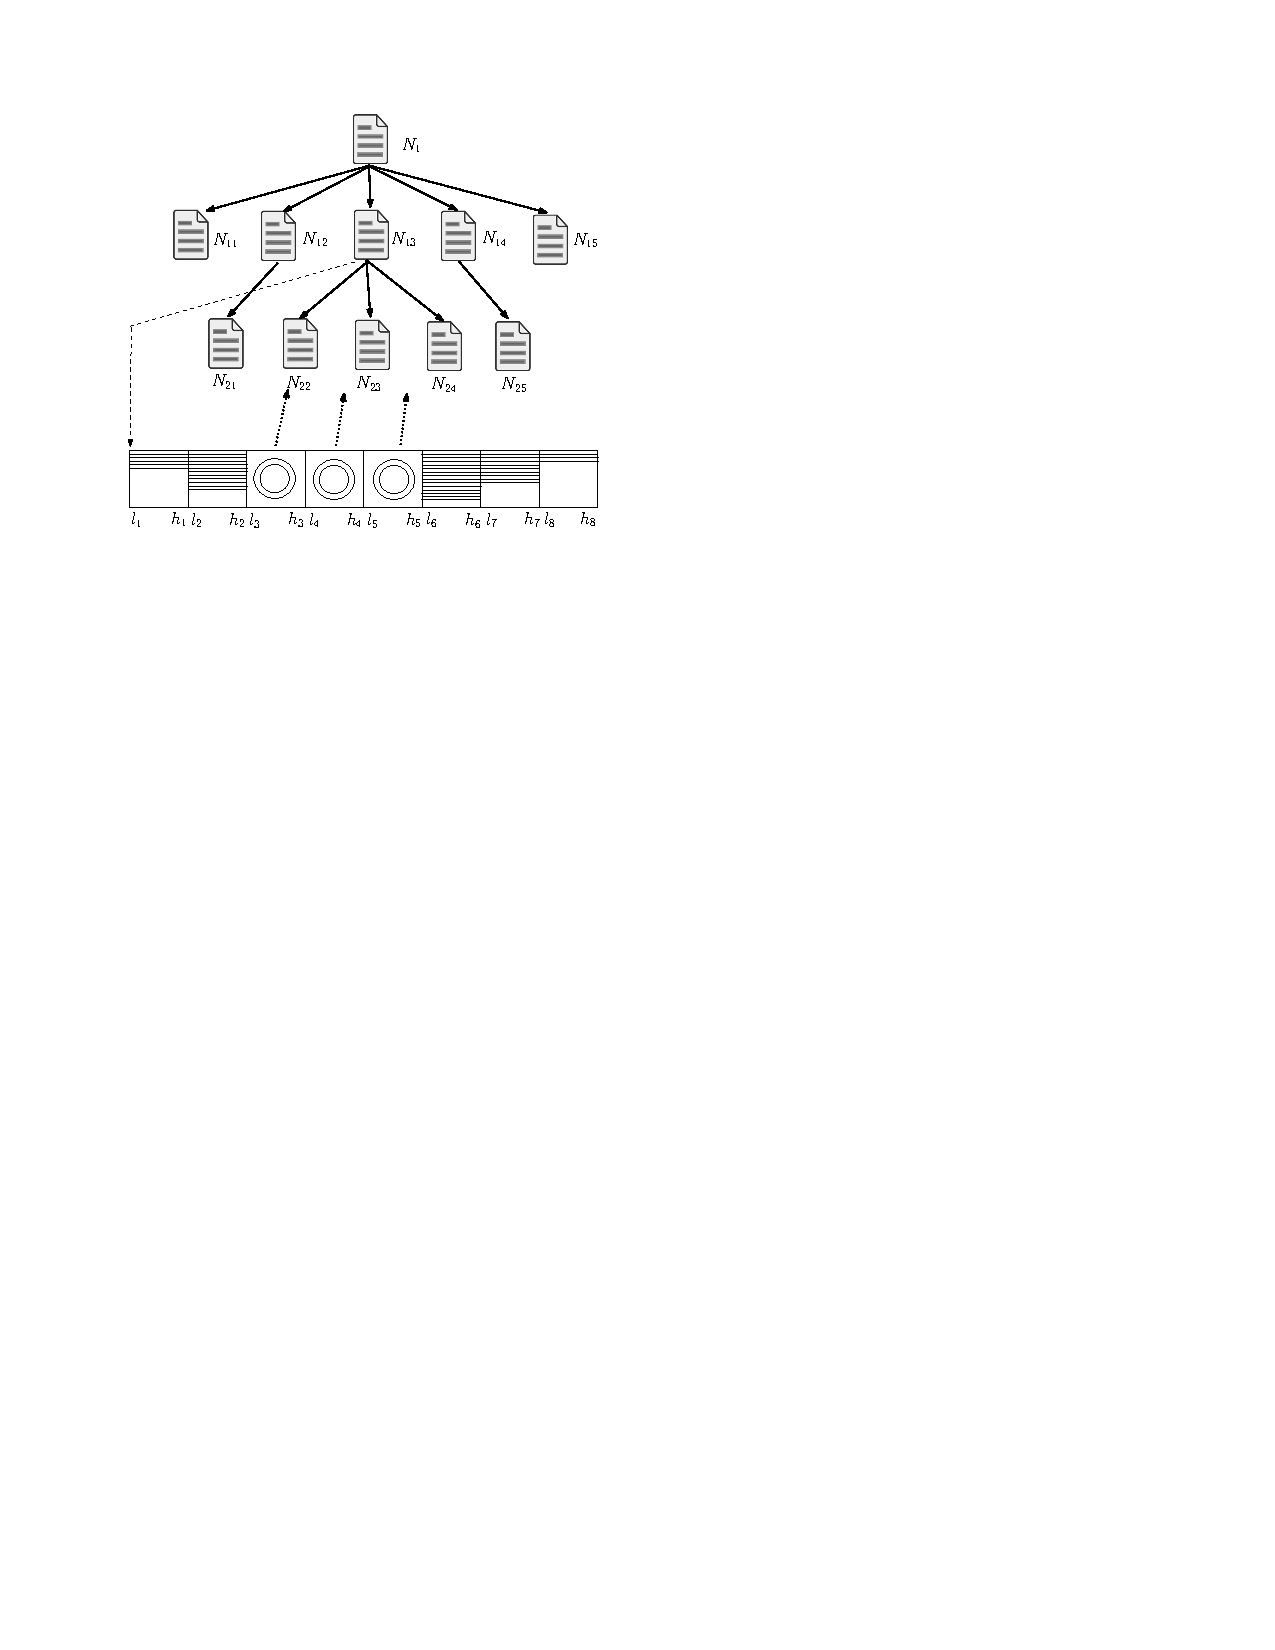
\includegraphics[width=0.65\columnwidth]{chapter2/hashfilestructure.pdf}
\caption{Estrutura del nodo HashFile. Figura adaptada de \cite{lshHashFile}.}
\label{fig:HashFile_structure}
\end{figure}

\newpage
\begin{lstlisting}[mathescape, frame=single, label=alg:HashFile,caption=Consulta kNN aproximada usando HashFile]
algorithm $ApproximateNN$($q, \lambda$)
    $init$ $\delta$
    $\delta$ := $ApproximateNNInNode$($q, root, \delta, \lambda$)
    return $\delta$
end.
procedure [$\delta$] = $ApproximateNNInNode$($q, node, \delta, \lambda$)
    $h_q := node.\textit{hash}(q)$
    for cada nodo $child$ do
        $wdist := |child.hash\_value - h_q|$
        if $wdist < \lambda$ then
            insertar $child$ en el $heap$ ordenado por $wdist$
        end if
    end for
    for cada página em disco $p_i$ do
        buscar la lista de paginas de $p_{start}$ a $p_{end}$ en disco entre los intervalos $[h_q - \lambda, h_q + \lambda]$
    end for
    cargar las páginas entre $[h_q - \lambda, h_q + \lambda]$ en el bloque $B$
    for cada objeto $o$ en $B$ do
        $dist := \|o - q\|_{L_2}$
        if dist < $\delta$ then
            $\delta := dist$
        end if
    end for
end.
\end{lstlisting}
\begin{comment}
\begin{lstlisting}[mathescape, frame=single, label=alg:HashFile,caption=Consulta kNN aproximada usando HashFile]
ApproximateNNInNode($q, node, \delta, \lambda$)
    $h_q = node.\textit{hash}(q)$
    for each child node $child$ do
        $wdist = |child.\textit{hash}value - h_q|$
        if $wdist < \lambda$ then
            add child to the heap ordered by $wdist$
    for each disk page $pi$ in increasing order do
        find the list of pages from $p_{start}$ to $p_{end}$ so that their intervals intersect with $[h_q - \lambda, h_q + \lambda]$
    load the $block$ of pages into memory
    for each object $o$ in the $block$ do
        $dist = \|o - q\|_{L_2}$
        if dist < $\delta$ then
            $\delta = dist$
    return $\delta$
end.
ApproximateNN($q, \lambda$)
    init $\delta$
    $\delta$ := ApproximateNNInNode ($q, root, \delta, \lambda$)
    return $\delta$
end.
\end{lstlisting}
\end{comment}

%\begin{figure}[h]
%\centering
% 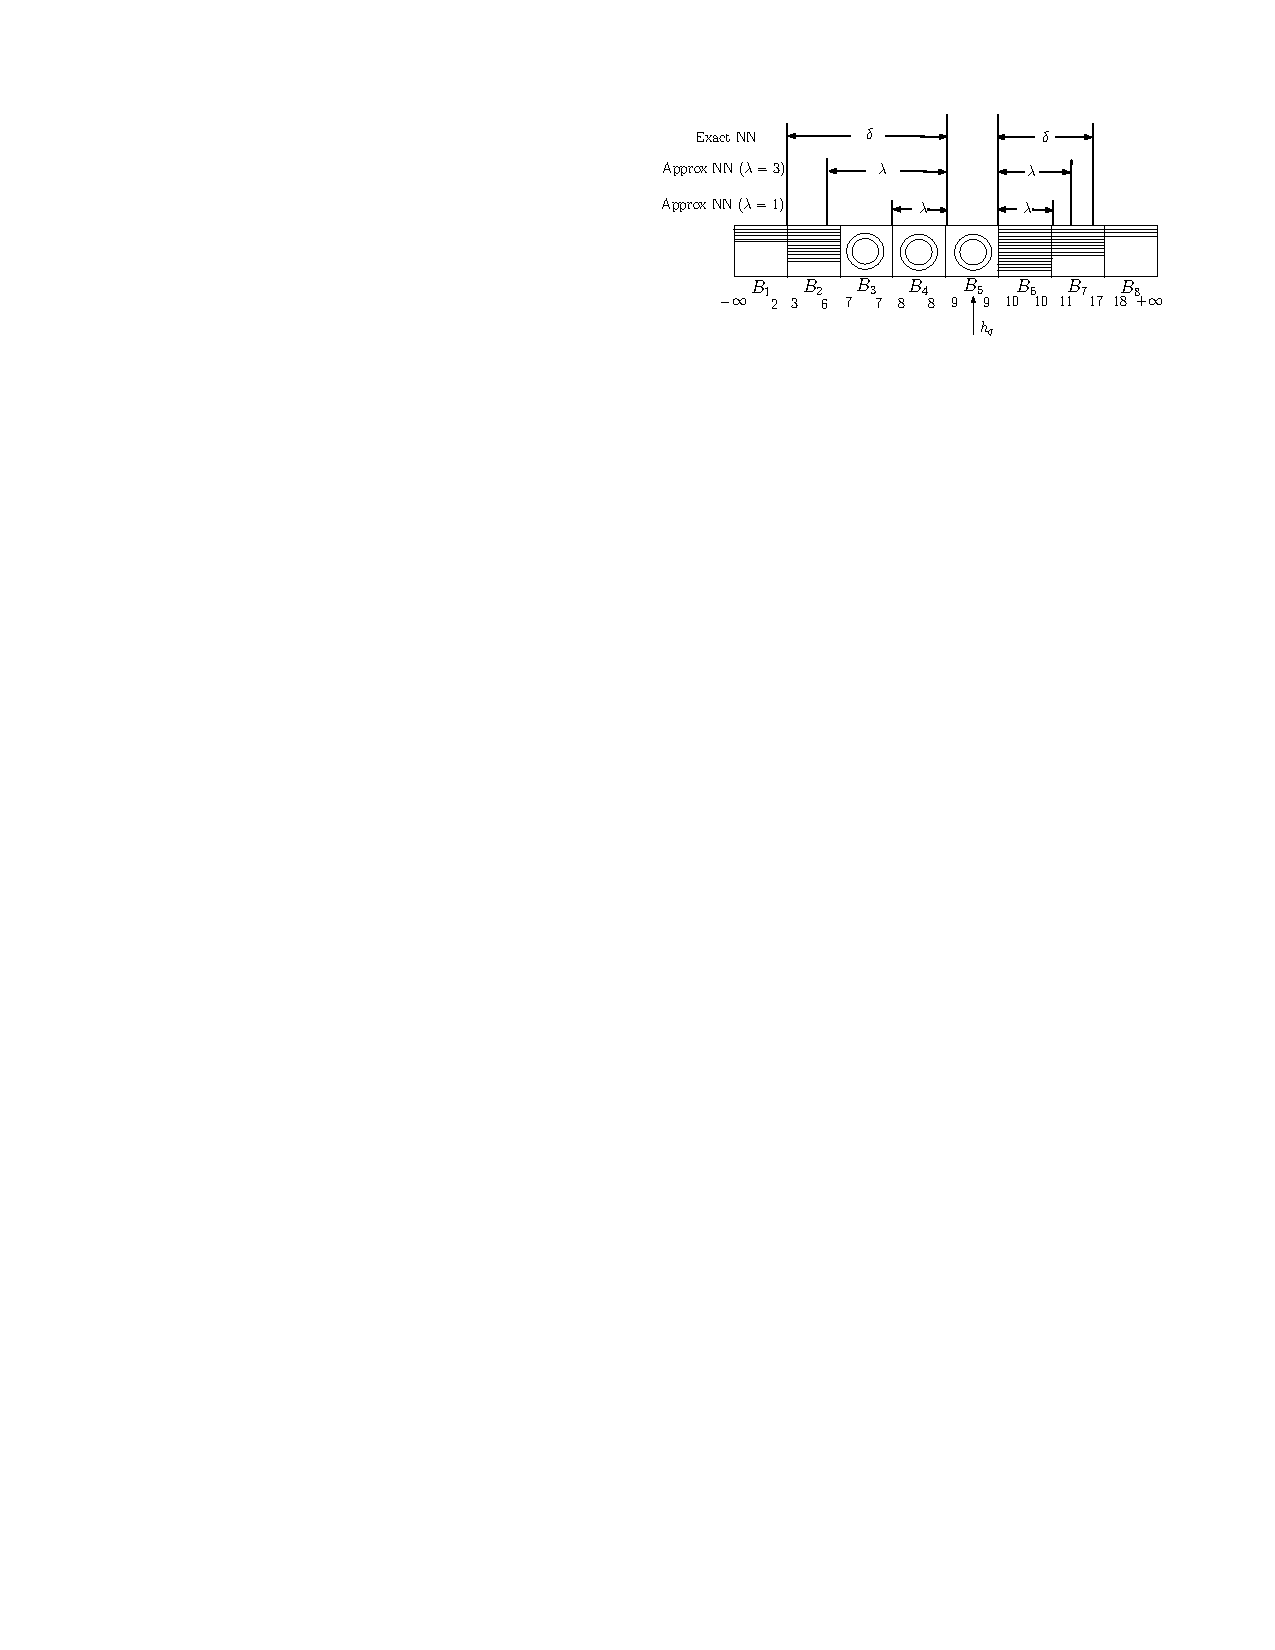
\includegraphics[width=0.7\columnwidth]{chapter2/hashfilequery.pdf}
%\caption{Busca kNN aproximada en un nodo  HashFile.  Figura adaptada de \cite{lshHashFile}.}
%\label{fig:HashFile}
%\end{figure}



\subsubsection{Consulta kNN Aproximada}
 
La Figura \ref{fig:cuda_NN_search} (a) presenta las proyecciones de una consulta por similitud aproximada en Hash-File, donde el objeto de consulta $q$ es mapeado usando las funciones \textit{hash} ($\mathcal{H}_1$ e $\mathcal{H}_2$) en los dos niveles de la estructura. Su estructura lógica correspondiente es presentada en la Figura \ref{fig:cuda_NN_search} (b). En este ejemplo, las proyecciones generan particiones diferentes en el espacio de búsqueda, donde cada función \textit{hash} es utilizada para organizar todo el conjunto de datos, de manera que la proximidad de objetos en el espacio original es mantenida en la proyección. Durante el procesamiento de la consulta, para cada una de las proyecciones el objeto de consulta q es proyectado para el valor \textit{hash} $h_q$, y apenas los objetos dentro del intervalo \textit{hash} $[ h_q - \lambda, h_q + \lambda]$  necesitan ser analizados. De este modo cada nivel contribuye en la precisión de los resultados ampliando el espacio de búsqueda.

\begin{figure}[ht]
 \centering
  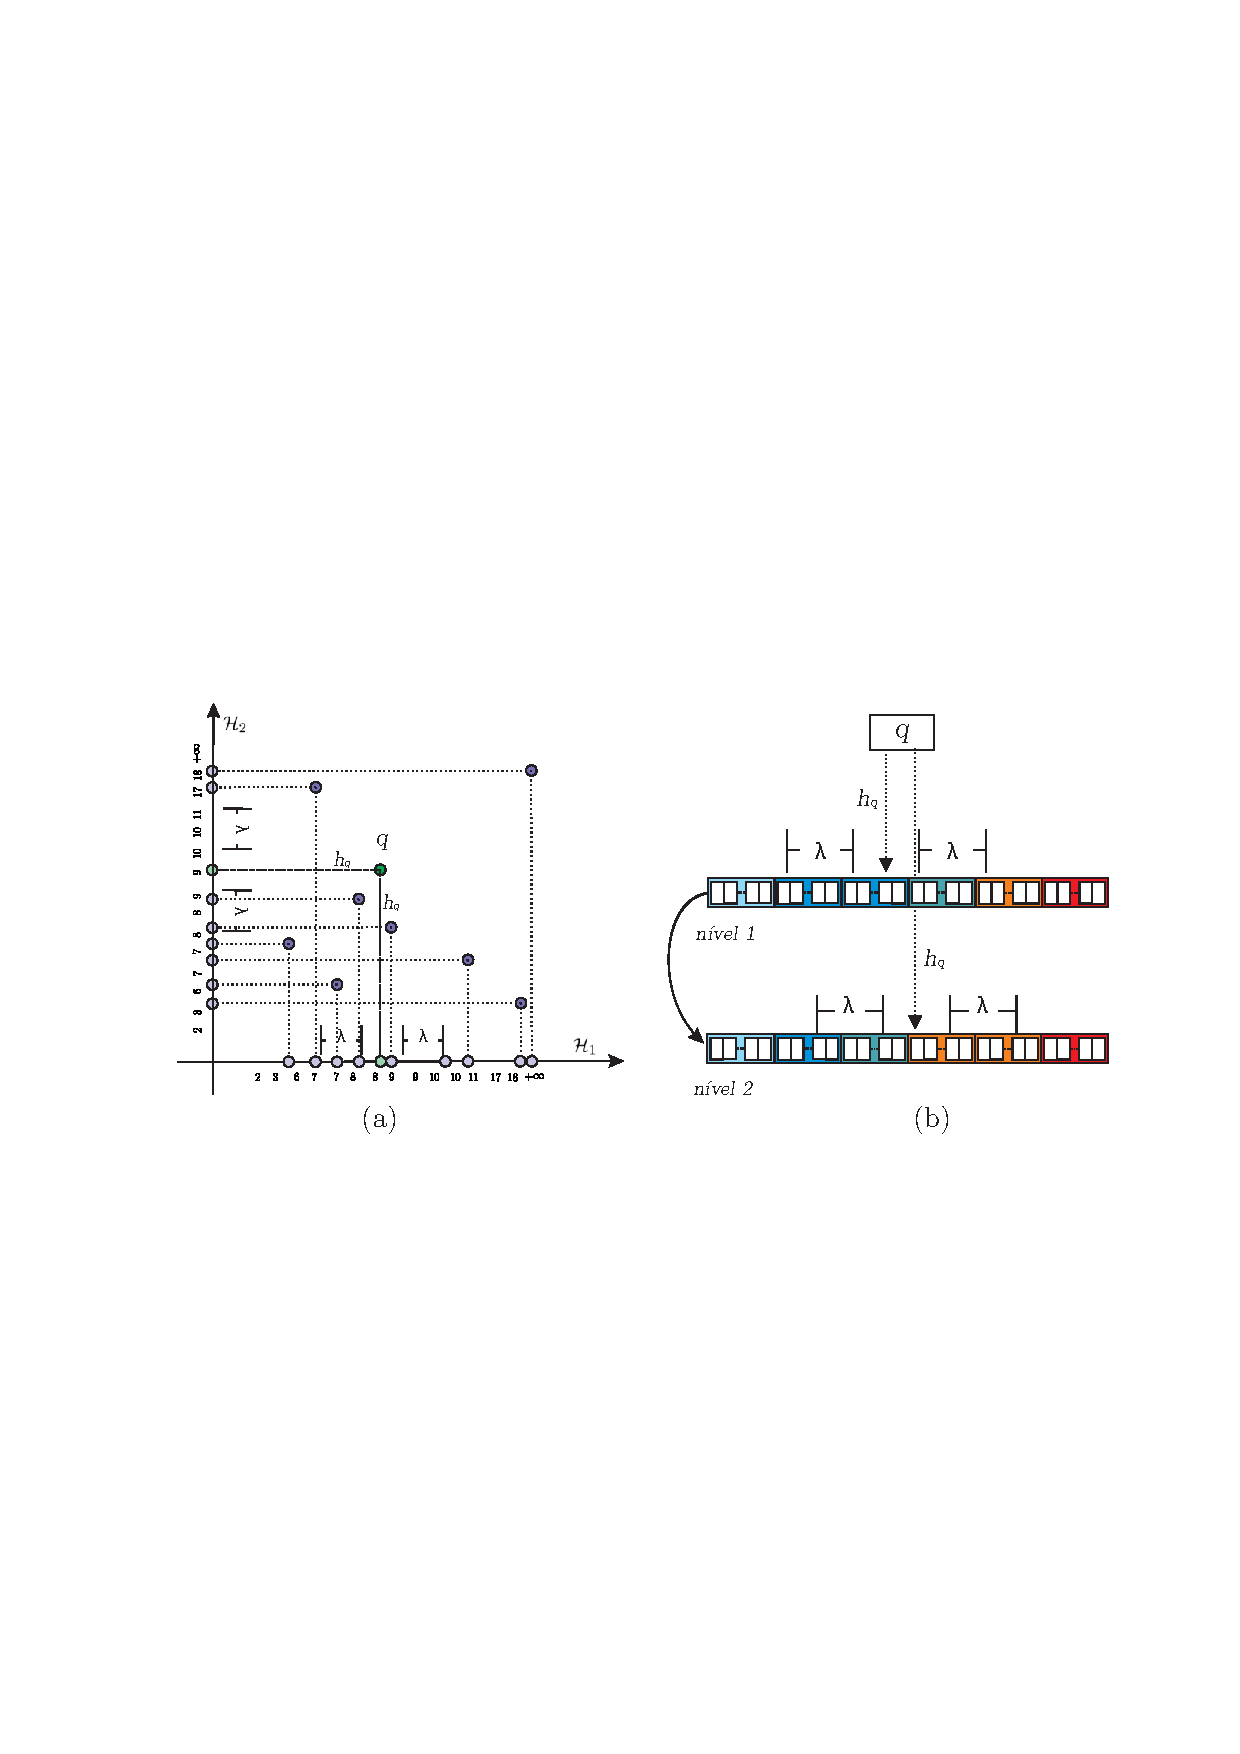
\includegraphics[width=0.99\columnwidth]{chapter2/cuda_hashfile.pdf}
 \caption{Representación de las proyecciones de una consulta por similitud aproximada en HashFile en (a), en (b) se verifica su estructura lógica correspondiente.}
 \label{fig:cuda_NN_search}
\end{figure}
  
Por otro lado, es  sabido que los hiperplanos que generar LSH tienden  poco  poder de discriminación conforme el numero de funciones \textit{hash} crece y además muchas tablas son requeridas para un nivel adecuado de precisión. Esta ineficiencia es debido a su naturaleza de procesamiento de manera independiente a los datos, donde los hiperplanos \textit{hash} son generado sin saber nada sobre la distribución de los datos.  Este problema  ha sido recientemente investigado en muchos métodos basados en \textit{hash} para permitir aprender funciones \textit{hash} adaptadas a la distribución de los datos. Estos métodos serán  discutidas en la siguiente sección. 

%\section{Otros métodos de codificación  para la búsqueda del vecino más cercano}
 
 %% FALTA AQUI UN RESUMEN :(
 
 
\section{Consideraciones Finales}

Como fue discutido en este capitulo,  soluciones exactas para  resolver el problema de búsqueda por similitud en altas dimensiones han sido estudiadas durante años, por otro lado algoritmos probabilísticos han sido poco explorados. De acuerdo con la literatura, es eficiente ejecutar consultas kNN exacta para datos en bajas dimensiones, mas en dimensiones altas las soluciones aproximadas son también una buena opción. El equilibrio entre la eficiencia y la eficacia se vuelve progresivamente más crítico conforme las dimensiones de los datos crece, debido a un fenómeno conocido como   la ``maldición  da la alta dimensionalidad''.

Muchas técnicas exactas y aproximadas, como los Métodos de Acceso Métricos (MAMs) y los métodos basados en \textit{Locality Sensitive Hashing} (LSH) y sus extensiones, fueron propuestas para resolver búsquedas en altas dimensiones.  Entre ellas, los métodos basado en LSH son de las pocas técnicas con garantía teórica de costo sub-linear. No obstante, muchas de sus implementaciones actuales presentan dificultades para ser implementados en problemas reales, como por ejemplo, tareas de minería de datos que dependen de algoritmo de búsqueda al vecino más próximo. He aquí el potencial de los métodos aproximados de búsqueda kNN.
 
%\chapter{Mineria de Datos \& Deep Learning }\label{cap:deep_learning}

\section{Consideraciones Iniciales}

Los rápidos avances en las tecnologías de recolección y de almacenamiento permitieron el almacenamiento de grandes cantidades de datos. Sin embargo, se probó que extraer conocimiento puede ser extremadamente desafiador. En este contexto, la minería de datos combina métodos tradicionales de análisis de datos con algoritmos sofisticados para el procesamiento de grandes volúmenes de datos \cite{Tan:2005:IDM:1095618}.

La Minería de Datos (Data Mining) es un área de investigación dentro en un contexto más amplio llamado Descubrimiento del Conocimiento en Bases de Datos (KDD – Knowledge Discovery in Databases), cuyo objetivo principal es extraer de un conjunto de datos, el conocimiento a ser utilizado en procesos decisorios. Más específicamente, los principales objetivos de los métodos de minería de datos son una descripción de un conjunto de datos y una predicción de valores futuros de interés basado en conocimiento previo de un banco de datos \cite{Fayyad:1996:DMK:257938.257942}.

  
 %%% corregir aqui :( 
 En la Sección \ref{sec:kdd-datamining} son discutidos los principales conceptos de Minería de Datos y Descubrimiento del Conocimiento en Bases de Datos (KDD), y como estos conceptos son adaptados para tomar en consideración la naturaleza de las series temporales. En la Sección \ref{sec:representacion-datos}, son presentados métodos de representación de datos. En la Sección \ref{sec:similitud-distancias}, se analizan las medidas de similitud y distancias. La Sección \ref{sec:similitud-series-temporales}, se analizan trabajos relacionados a consultas por similitud en series temporales. En la Sección \ref{sec:motif-discovery} se describe a profundidad algunos principios propuestos para resolver el descubrimiento de \textit{motifs}. Que junto con las consultas por similitud, son las actividades más relevantes del trabajo. La Sección \ref{sec:clustering} son discutidos los principales conceptos de Clustering de Datos. La Sección \ref{sec:clasificacion} describe los conceptos de clasificación de datos. La Sección \ref{sec:outlier} presenta el análisis de Outliers, que son anomalías, discordancias o desviaciones en la minería de datos. En la Sección \ref{sec:data-streams} se presenta conceptos de data streams. La Sección \ref{sec:evaluacion-validacion} describe métodos de evaluación y validación utilizados en los resultados del proceso de KDD. La Sección \ref{subsec_precis_recall} describe el reconocimiento de formas, y en la Sección \ref{sec:consideraciones-finales} se presentan las consideraciones finales del capítulo.


\section{KDD y Mineria de Datos}\label{sec:kdd-datamining}

\textbf{Descubrimiento de Conocimiento en Base de Datos (KDD)} - es el proceso de: primero, a partir de los datos, identificar patrones válidos, nuevos, potencialmente útiles y comprensivos. Segundo \cite{Fayyad:1996:DMK:257938.257942}, este proceso está compuesto de cinco etapas: selección de los datos; pre procesamiento y limpieza de los datos; transformación de los datos; Minería de los Datos (\textit{Data Mining}); e interpretación y validación de los resultados. La interpretación entre estas diversas etapas puede ser observada en la Figura \ref{fig:processoKDD}, siendo que las tres primeras pueden ser interpretadas como un análisis exploratorio de los datos.

\begin{figure}[htp]
\centering
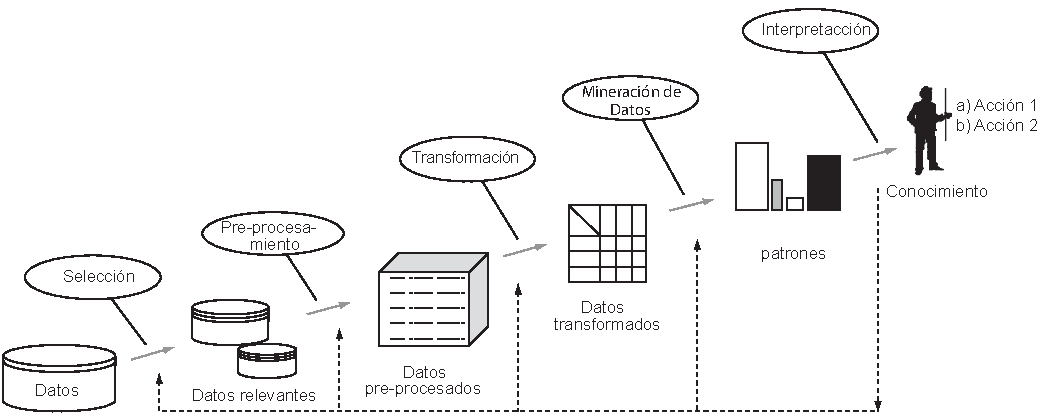
\includegraphics[width=0.99\columnwidth]{Parte3/design/KDD-process.pdf}
\caption{Etapas del proceso KDD. Figura adaptada de \cite{Fayyad:1996:DMK:257938.257942}.}
\label{fig:processoKDD}
\end{figure}


Los principales pasos para el proceso de KDD son:

\begin{enumerate}

    \item \textbf{Limpieza de datos:} Las bases de datos del mundo real a menudo tienen datos incompletos, con ruido e inconsistentes que pueden dañar el análisis dificultando la detección de patrones. Los procedimientos de limpieza de datos trabajan para preparar los datos para los siguientes pasos en el procesos KDD mediante el llenado de los valores que faltan, corrigiendo los datos con ruido, identificando y removiendo valores atípicos, y resolviendo inconsistencia.
    \item \textbf{Integración de datos:} En algunas circunstancias, los datos de múltiples fuentes deben fusionarse y transformadas en formas apropiadas para ser incluidas en el mismo análisis. Por lo tanto, este paso implica técnicas para integrar correctamente múltiples bases de datos, cubos de datos o archivos en un almacenamiento de datos.
    \item \textbf{Selección de datos:} Este paso corresponde a la identificación de datos relevantes para la tarea de análisis y su recuperación a partir de las bases de datos.
    \item \textbf{Transformación de datos:} En este paso, los datos son transformados o consolidados en adecuadas formas para la extracción usando operaciones, tales como el resumen, la agregación, la generalización o la normalización.
    \item \textbf{Minería de datos:} Este paso es fundamental en el proceso KDD, donde se aplican técnicas computacionales para extraer patrones desconocidos y útiles a partir de los datos.
    \item \textbf{Evaluación del patrón:} En este paso, se utilizan medidas interesantes para identificar los patrones que representan el conocimiento.

\end{enumerate}


La etapa de minería de datos incluye la definición de las tareas de minería a ser realizadas, la elección del algoritmo a ser aplicado y la extracción de patrones de interés. En la etapa siguiente, los patrones son interpretados y validados, y si los resultados no fueran satisfactorios (validos, nuevos, útiles y comprensibles), el proceso retorna a uno de los dos estados anteriores. Caso contrario, el conocimiento descubierto es consolidado \cite{Fayyad:1996:DMK:257938.257942}. El proceso KDD se refiere a todo el proceso de descubrimiento de conocimiento útil para los datos, en cuanto a la Minería de los Datos se refiere a la aplicación de algoritmos para extraer modelos de los datos.


\section{Aprendizaje de Máquina -- \textit{Machine Learning} }

    Durante las últimas décadas el aprendizaje de maquina se ha convertido en uno de los pilares de la tecnología de la información y con ello, a llegado a formar parte importante de nuestras vidas, aunque de manera imperceptible. Con la gran cantidad de datos que se generan constantemente, hay razones suficientes para creer que el análisis inteligente de datos será cada vez más generalizado como un ingrediente necesario para el progreso tecnológico, \cite{smola2008ml}.

    \subsection{Maquinas Inteligentes}

    El cerebro es el órgano del cuerpo humano mas increíble. Este determina la forma en la que percibimos el mundo con nuestros sentidos. Desde niño el ser humanos es capas de  resolver problemas que incluso los supercomputadores más potentes no pueden resolver. Por décadas el ser humano a soñado por construir maquinas inteligentes con conciencia como la nuestra, asistentes robóticas para limpieza de nuestros hogares, autos que se manejan por si solos, microscopios que automáticamente detectan enfermedades. Pero la construcción de estas máquinas de inteligencia artificial nos obliga a resolver algunos de los problemas más complejos de la ciencia con los que hemos tenido que lidiar, comprender el funcionamiento de nuestros cerebros. \cite{dlBook}.

    \subsection{Mecanismos del aprendizaje de maquina}

    Para hacer frente a esta clase de problemas tendremos que utilizar un tipo muy diferente de enfoque. Muchas de las cosas que aprendemos en la escuela tienen mucho en común con los programas informáticos tradicionales. Aprendemos cómo multiplicar números, resolver ecuaciones, y hacer derivadas mediante la guía de un conjunto de instrucciones. Pero las cosas que aprendemos a una edad muy temprana, las cosas que nos parecen naturales, se aprenden con el ejemplo, no por fórmulas \cite{dlBook}.
    \\\\
    Deep Learning es un subconjunto de un campo más amplio de la inteligencia artificial llamado aprendizaje de maquina o \textit{Machine Learning}, que se basa en la idea de aprender con el ejemplo. En lugar de enseñar a una computadora las reglas para resolver un problema, le damos un modelo con el que se puede evaluar ejemplos y un pequeño conjunto de instrucciones para modificar el modelo cuando se comete un error. Esperando que, con el tiempo, un modelo fuera capaz de resolver el problema con gran precisión \cite{dlBook}.
    \\\\
    Ahora formularemos esta idea matemáticamente, vamos a definir nuestro modelo como una función $h(X,\theta)$ la entrada $X$ es un ejemplo expresado en forma de vector. Por ejemplo, si $X$ fuera una imagen en escala de grises, los componentes del vector serían las intensidades de los píxeles en cada posición, como se muestra en la Fig.~\ref{fig:gscale}.
    \begin{figure}[htp]
        \centering
        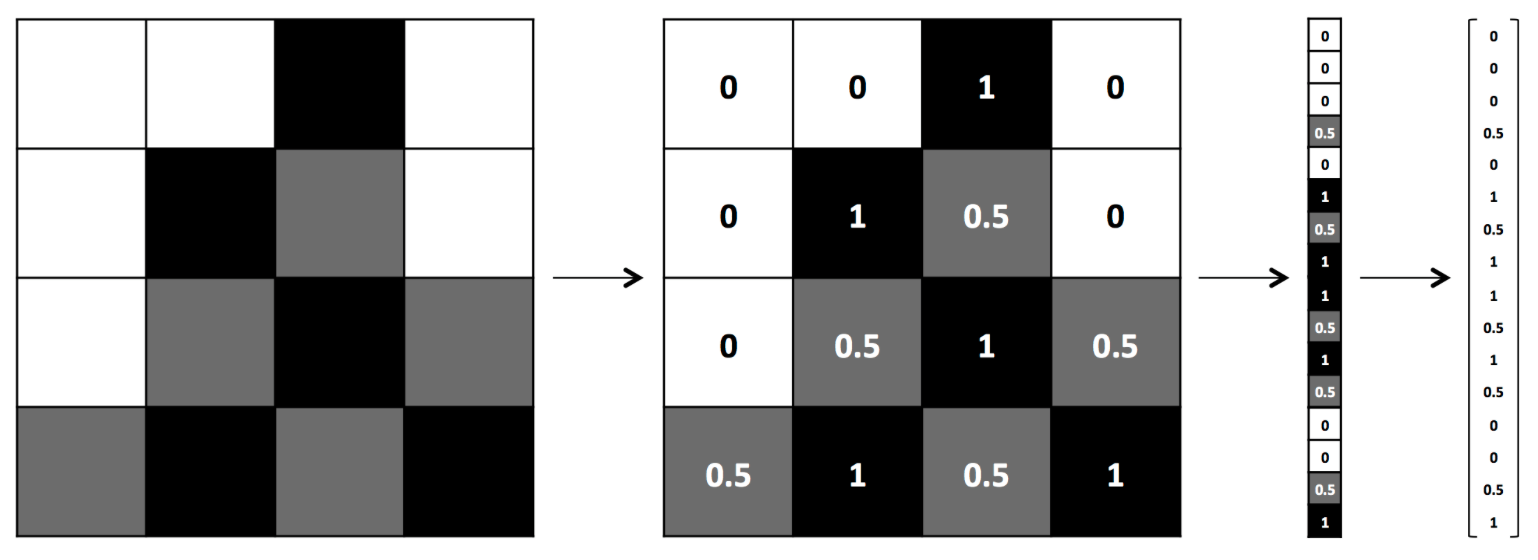
\includegraphics[scale=0.3]{mteorico/grayscale.png}
        \caption{Vectorización de una imagen}
        \source{Fundamentals of Deep Learning, \cite{dlBook}}
        \label{fig:gscale}
    \end{figure}

    La entrada $\theta$ es un vector de parámetros que utiliza nuestro modelo, este intenta perfeccionar los valores de estos parámetros, ya que se expone a más y más ejemplos. Para comprender mejor los modelos de aprendizaje de maquina, analizaremos un ejemplo, digamos que pretendemos determinar cómo predecir el rendimiento en un examen, basándonos en el número de horas de sueño y el número de horas de estudio del día anterior. Recolectamos muchos datos y para cada punto de los datos tenemos que $X=[x_1\ x_2]^T$, registraremos la horas de sueño en $x_1$, las horas de estudio en $x_2$ y nuestro desempeño, ya sea sobre o por debajo del promedio de la clase. Entonces, nuestro objetivo seria entrenar un modelo $h(X,\theta)$ con un vector $\theta=[\theta_1\ \theta_2\ \theta_3]$ tal que:

    \begin{equation}
        h(X,\theta)\begin{cases}-1 & if\ x^T.\begin{bmatrix}\theta_2\\\theta_3 \end{bmatrix}+\theta_1< 0\\1 & if\ x^T.\begin{bmatrix}\theta_2\\\theta_3 \end{bmatrix}+\theta_1 \geq 0\end{cases}
    \end{equation}

    En otras palabras, se puede suponer que el esquema para nuestro modelo $h(X,\theta)$ es como se describió anteriormente (geométricamente, este esquema, describe un clasificador lineal que divide el plano de coordenadas en dos mitades). Entonces, ahora se desea entrenar el vector $\theta$ de modo que el modelo haga predicciones correctas (-1 para valores por debajo de la media, y 1 en caso contrario) dado un ejemplo de entrada $X$. Este modelo es llamado perceptron lineal, podemos asumir que nuestros datos están distribuidos como se muestra en la Fig.~\ref{fig:sdata}.
    \\\\
    Si seleccionamos $\theta=[-24\ 3\ 4]$, nuestro modelo de aprendizaje hace una predicción correcta según el siguiente modelo:

    \begin{equation}
        h(X,\theta)\begin{cases}-1 & 3x_1+ 4x_2-24< 0\\
        1 &  3x_1+ 4x_2-24 \geq 0\end{cases}
    \end{equation}
    \\
    Un vector de parámetros $\theta$ posiciona correctamente el clasificador por lo que se pueden realizar predicciones correctas. En la mayoría de los casos, hay muchos (o incluso un número infinito) posibles opciones para $\theta$ que son óptimas. Afortunadamente para nosotros, la mayoría de las veces estas alternativas están tan cerca una del otra que la diferencia en su rendimiento es insignificante. Si este no fuera el caso, podemos utilizar más datos para nuestra elección de $\theta$, \cite{dlBook}.
    \begin{figure}[htp]
        \centering
        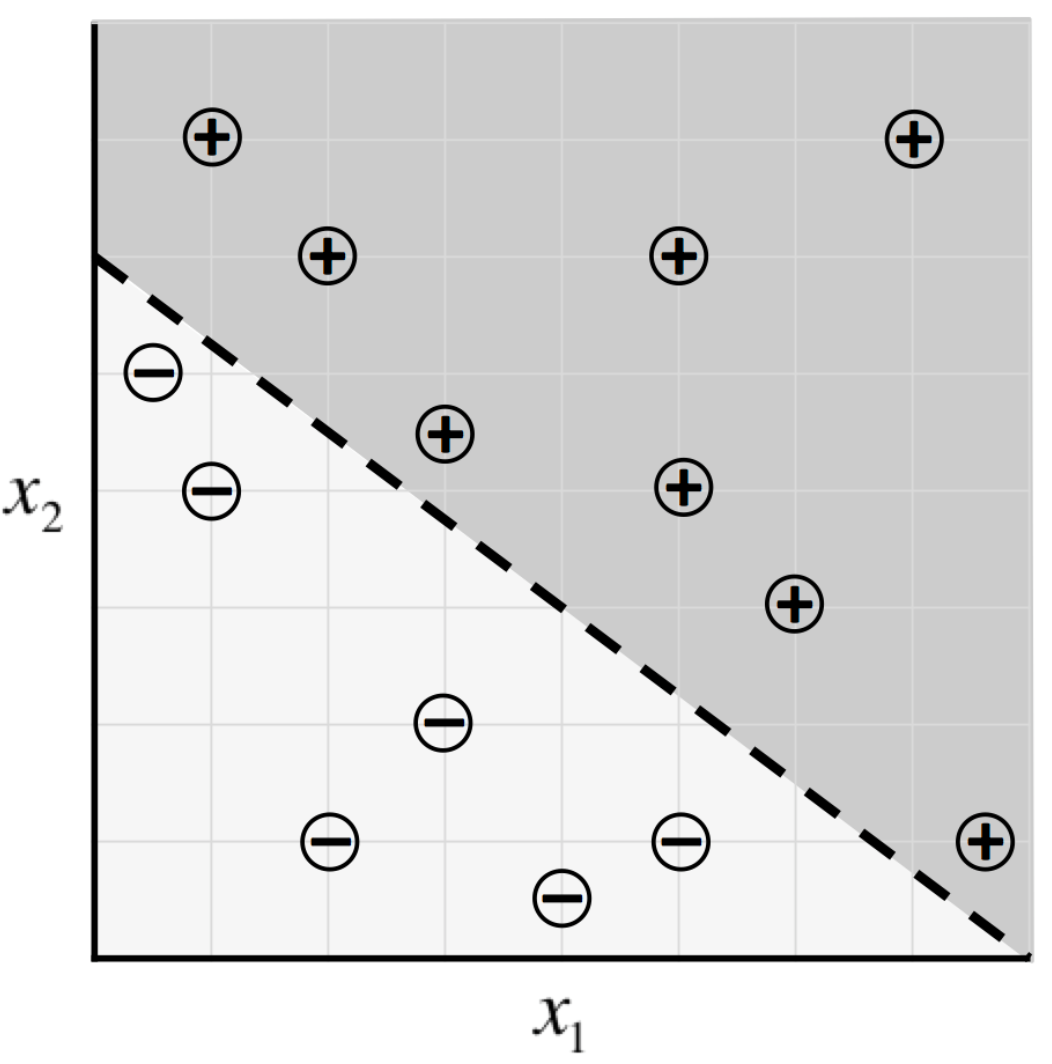
\includegraphics[scale=0.23]{mteorico/sampleData.png}
        \caption{Ejemplo de clasificador lineal}
        \label{fig:sdata}
        \source{Fundamentals of Deep Learning, \cite{dlBook}}
    \end{figure}

% \section{Reconocimiento de patrones}



\section{Redes Neuronales}

    Clasificadores polinómicos pueden modelas superficies de decisión, sin embargo su utilidad en la practica es limitada, debido a la facilidad con la que se sobre entrena con datos de entrenamiento ruidosos y la alta dimensionalidad de los datos. Mejores resultados pueden obtenerse con redes neuronales artificiales, donde muchas unidades simples, llamadas neuronas, están interconectadas por enlaces denominados pesos, estos forman parte de estructuras mas grandes de alto rendimiento, \cite{kubat2015introduction}.

    % Una arquitectura de red o topología juega un papel importante para la clasificación, la topología óptima dependerá del problema en cuestión. A menudo el conocimiento del dominio del problema que podría ser de carácter informal o heurística puede incorporarse fácilmente en la arquitectura de redes a través de opciones, como número de capas ocultas, unidades, conexiones de retroalimentación. Por lo tanto el establecimiento de la topología de la red es la selección del modelo heurístico. La facilidad práctica en la selección de modelos (topologías de red) y la estimación de parámetros (formación a través de propagación hacia atrás) permiten a los diseñadores de clasificadores probar modelos alternativos de manera bastante simple. \cite{PattClassi}


    \subsection{Neurona y Red de Neuronas}

    La unidad fundamental del cerebro es la neurona, cada una de las cuales forma una media de 6.000 conexiones con otras neuronas. Es esta red biológica masiva que nos permite experimentar el mundo que nos rodea. De esta manera podemos trasladar esta concepto funcional de las neuronas de nuestro cerebro en un modelo artificial que podemos representar en nuestro computador. Aunque las neuronas artificiales pueden ser muy poderosas, es imposible que una sola neurona pueda realizar tareas complejas. Así que para hacer frente a esto, las neuronas deben organizarse por capas al igual que las neuronas del cerebro humano. De hecho, la corteza cerebral humana está conformada por capas. Los flujos de información pasan de una capa a otra hasta que la entrada sensorial se convierte en la comprensión conceptual. Por ejemplo, la parte más baja de la corteza visual recibe datos visuales de los ojos. Esta información es procesada por cada capa y se pasa a la siguiente hasta la ultima capa, donde se define lo que se esta observando, \cite{dlBook}.

    \subsection{Neuronas Sigmoidales, Tanh y ReLU}

    Hay tres principales tipos de neuronas que se utilizan en la práctica que introducen no linealidad en sus cálculos. El primero de ellos es la neurona \textit{sigmoide}, que utiliza la función:

    \begin{equation}
        f(z)=\frac{1}{1+e^{-z}}
    \end{equation}
    \\
    Intuitivamente, esto significa que cuando la salida es muy pequeña, la activación de la neurona está muy cerca de 0. Cuando la salida es muy grande, la activación de la neurona está cerca de 1 y entre estos dos extremos, la distribución de los datos asumen una forma distintiva, como se muestra en la Fig.~\ref{fig:sigmoide}
   

    La función de activación \textit{Tanh} utiliza la misma distribución como se observa en la Fig.~\ref{fig:tanh}, pero en lugar de un rango de 0 a 1, la salida de las neuronas \textit{Tanh} van desde -1 a 1. Como era de esperar, este utiliza la función $f(z)=tanh(z)$. La función de activación \textit{Tanh} es preferida sobre la activación \textit{sigmoide} ya que esta mantiene el cero como centro \cite{dlBook}.
 
    La función de activación \textit{Restricted Linear Unit} (ReLU), es una nueva clase de no linealidad, esta usa la función $f(z)=max(0,z)$, que da como resultado la Fig.~\ref{fig:relu}.  \cite{dlBook}. En otras palabras, la activación es simplemente un funcion que aplica un umbral en cero.
 

    \subsection{Capa de salida Softmax}

    Este tipo de capa es utilizada cuando se desea que un vector de salida sea una distribución de probabilidad sobre un conjunto de etiquetas que se excluyen mutuamente. Por ejemplo, si se construye una red neuronal para reconocer los dígitos escritos a mano a partir del conjunto de datos MNIST. Cada una de las etiquetas (0 a 9) se excluyen mutuamente, pero aun así es poco probable poder reconocer el 100\% de los dígitos. El uso de una distribución de probabilidad proporciona una mejor idea respecto a las predicciones obtenidas. Como resultado, el vector de salida deseado es de la siguiente forma $\sum_{i=0}^9 p_i=1$, donde $p_i=[p_1\ p_2\ ...\ p_9]$.
    \\\\
    Esto se logra mediante el uso de una capa de salida especial llamado \textit{softmax}. A diferencia de otros tipos de capas, la salida de una neurona en una capa \textit{softmax} depende de las salidas de todas las otras neuronas en su capa. Esto se debe a que se requiere que la suma de todas las salidas sea igual a 1. Podemos lograr esta normalización ajustando su salida con la siguiente función:

    \begin{equation}
        \centering
        y_i=\frac{e^{x_i}}{\sum_k e^{x_k}}
    \end{equation}
    \\\\
    Una predicción de alta precisión tendría una única salida del vector cercano a 1, mientras que las salidas restantes estarían cerca a 0. Una predicción débil tendría varias etiquetas más o menos con la misma probabilidad \cite{dlBook}.


% \section{Perceptron Multicapa}

%     \section{Feed-Forward Neural Networks}

%     Lo mas importante de una red neuronal es encontrar el vector de $\theta$. Esto se logra mediante un proceso comúnmente conocido como entrenamiento. Durante el entrenamiento, mostramos a la red neuronal un gran número de ejemplos de entrenamiento y de forma iterativa ajustamos los pesos y reducimos al mínimo los errores. Después de muchos ejemplos, esperamos que nuestra red neuronal sea muy eficaz en la solución de la tarea para la que ha sido entrenada.
%     \\\\
%     Para comprender el proceso de entrenamiento imaginemos el siguiente ejemplo, todos los días, compramos una comida del comedor que consta de hamburguesas, patatas fritas y refrescos. Compramos un número de porciones de cada elemento y queremos ser capaces de predecir la cantidad de dinero que nos va a costar, pero los elementos no tienen etiquetas de precio. Lo único que el cajero nos dirá es el precio total de la comida. Queremos formar una sola neurona lineal para resolver este problema. ¿Cómo lo hacemos?

\section{Redes Neuronales Convolutivas (CNN)}

Una red neuronal convolucional (CNN) es una arquitectura jerárquica \cite{LeCun} que consta de varias capas convolucionales apiladas (opcionalmente seguido por una capa de normalización y una capa de agrupación), capas completamente conectadas y una capa de salida en la parte superior. Las capas convolucionales generan mapas de características por filtros convolucionales lineales seguidos por funciones de activación no lineales (Rectificador, Sigmoide, TanH, etc.). La capa completamente conectada (\textit{fully conected layer}) tiene conexiones completas a todas las activaciones en los mapas de características y el vector unidimensional resultante se puede alimentar en la capa de salida para la optimización de la función de pérdida.

Hay dos etapas principales para entrenar la red neuronal convolucional: una etapa \textit{fordward}  y una etapa de \textit{backward}.  En primer lugar, la etapa de \textit{fordward} es representar la imagen de entrada con los parámetros actuales (pesos y sesgo/bias) en cada capa. A continuación, la salida de la última capa se utiliza para calcular la función de pérdida con las etiquetas de verdad. En segundo lugar, basándose en el costo de la pérdida, la etapa \textit{backward} calcula los gradientes de cada parámetro con reglas de cadena. Todos los parámetros se actualizan en función de los gradientes y se preparan para el siguiente cálculo directo. Después de suficientes iteraciones de las etapas \textit{fordward} y \textit{backward}, la red podría ser optimizada. La red neuronal convolucional ha sido aplicada en diversas aplicaciones de visión por computadora y ha demostrado sus ventajas significativas y alto rendimiento.

\subsection {Tipos de capas CNN}

En esta seccion presentamos una visión general de los diferentes tipos de capas y luego revisaremos brevemente las aplicaciones de visión computacional basadas en CNN.

\textbf{Capas convolucionales(\textit{Convolucional layers}):} Las capas convolucionales de la arquitectura CNN utilizan $k$ filtros (o núcleos) para envolver la imagen de entrada para generar $k$ mapas de características. Hay tres ventajas principales de la operación de convolución \cite{Zeiler}: en primer lugar, el mecanismo de reparto de parámetros se utiliza en capas convolucionales de tal manera que el número de parámetros podría reducirse significativamente. En segundo lugar, la conectividad local aprende correlaciones entre píxeles vecinos. En tercer lugar, es invariante a la ubicación del objeto. Debido a estos beneficios introducidos por la operación de convolución, algunos trabajos de investigación bien conocidos también lo utilizan como un reemplazo de las capas totalmente conectadas para acelerar el proceso de aprendizaje \cite{Szegedy,Oquab}.

\textbf{Capas de agrupamiento(\textit{Pooling layers}):} Una capa de agrupación es una capa opcional que sigue una capa convolucional que sub-muestrea su entrada. La agrupación media(\textit{average pooling}) y la agrupación máxima(\textit{max pooling}) son las operaciones de agrupación más utilizadas. La razón para utilizar una operación de agrupación en la red neuronal convolucional es que: en primer lugar, puede reducir las dimensiones de la salida y el número de parámetros de la red, manteniendo la información más destacada. En segundo lugar, una operación de agrupación también proporciona una invariancia básica para la traducción (desplazamiento) y la rotación.  Para un \textit{max pooling}g y \textit{average pooling}, Boureau et al. \cite{Boureau} proporcionó un análisis teórico detallado de su funcionamiento. Scherer et al. \cite{Scherer} realizó una comparación entre las dos operaciones de agrupación y encontró que \textit{max pooling} puede conducir a una convergencia más rápida, selección de características invariantes superiores y mejorar la generalización.

\textbf{Capas completamente conectadas(\textit{Fully-connected layers}):}  Después de varias capas convolucionales y de agrupación máxima, el razonamiento de alto nivel en la red neuronal convolucional se realiza a través de las capas completamente conectadas. Una capa completamente conectada toma todas las neuronas de la capa anterior (ya sea totalmente conectado, agrupación o convolucional) y lo conecta a cada neurona que tiene. Las capas completamente conectadas no estan espacialmente localizados , ya que los mapas de características de entrada se convierten en un vector de características unidimensional. El vector de característica unidimensional podría alimentar el \textit{forward} del vector en una capa de pérdida o tomarlo como una representación característica para el procesamiento de seguimiento \cite{Girshick}. El inconveniente de la capa totalmente conectada es que contiene muchos parámetros, lo que da lugar a grandes costes computacionales y de almacenamiento. Por lo tanto, GoogleNet \cite{Szegedy} diseñó una red profunda y amplia, manteniendo el costo computacional constante, cambiando de arquitectura totalmente conectado a escasamente conectadas. La arquitectura \textit{Network in Network} (NIN) \cite{Lin} reemplaza la capa completamente conectada por una capa de agrupación media \textit{average pooling} global.


\subsection {Aplicaciones de   {Redes Neuronales Convolutivas (CNN)}}

Recientemente, el aprendizaje profundo, especialmente para las CNN, produjo el estado del arte de rendimiento en diversas aplicaciones de visión computacional, tales como clasificación de imágenes, búsqueda de imágenes, detección de objetos, segmentación de imágenes semánticas, estimación de la postura humana, etc.

\textbf{Clasificación de imágenes:} Krizhevsky et al. \cite{Krizhevsky} establece un hito para la clasificación de imágenes a gran escala cuando el entrenamiento de una gran CNN en el conjunto de datos ImageNet \cite{Deng}, lo que demuestra que CNN podría funcionar bien en la clasificación de imagen natural. OverFeat \cite{Sermanet} propuso un marco de ventana multi-escala y deslizante, que podría encontrar la escala óptima de la imagen y cumplir tareas diferentes simultáneamente, por ejemplo, clasificación de imágenes, detección de objetos y localización. Debido a que las CNN existentes requieren datos de imagen de tamaño fijo como entrada, el modelo SPP-Net eliminó esta restricción mediante una estrategia espacial de agrupación de pirámides en las CNN y mejoró la precisión de clasificación de una variedad de arquitecturas CNN a pesar de sus diferentes diseños.  La propuesta posterior de VGGNet \cite{Simonyan} y Google Net \cite{Szegedy} mejoró significativamente el rendimiento de la clasificación de imágenes al aumentar el ancho y la profundidad de las arquitecturas de red.

\textbf{Detección de objetos: }Un esquema general para sistemas de detección de objetos de alto rendimiento es generar un gran número de propuestas de la región del objeto candidato y clasificarlas utilizando sus características CNN de alto rendimiento. El enfoque más representativo son las regiones con características CNN (RCNN) \cite{Girshick}. Utiliza la búsqueda selectiva \cite{Uijlings} para generar propuestas de región de objetos y extrae las características de CNN para cada región candidata. Las características se introducen en un clasificador SVM para decidir si las ventanas candidatas relacionadas contienen el objeto o no. RCNNs mejoró el punto de referencia de la detección de objetos por un gran margen, y se convirtió en el modelo base para muchos otros algoritmos prometedores \cite{Hariharan,Zhu,Zhang}. Además, los RCNN originales eran computacionalmente caros, los trabajos recientes \cite{He,GirshickR} emplearon la estrategia de compartir convoluciones en las propuestas de la región para reducir el coste de cálculo. Los últimos frameworks de Fast RCNN \cite{GirshickR} y Faster RCNN \cite{Ren} logran tasas casi en tiempo real utilizando redes muy profundas.

\textbf{Recuperación de imágenes:} :El éxito de AlexNet \cite{Krizhevsky} sugiere que las CNN pueden ser usadas como extractoras de características de alto nivel y universales. Las características emergentes en las capas totalmente conectadas de la CNN pueden servir como una representación de imagen de alto nivel para la clasificación de imágenes. Motivado por esto, muchos estudios recientes hacen uso de las activaciones de las capas superiores totalmente conectadas en CNNs para la recuperación de imágenes \cite{Gong,Liu,Sharif,Wan,Sun,Babenko}. Investigaciones recientes también sugieren explorar las características de las capas convolucionales profundas en CNNs. Estas características tienen propiedades muy útiles: en primer lugar, se pueden extraer eficientemente de una imagen de cualquier tamaño y relación de aspecto. En segundo lugar, las características de las capas convolucionales tienen una interpretación natural como descriptores de regiones de imágenes locales correspondientes a campos receptivos de las características particulares. Por último, las operaciones de agrupación simple puede agregar mapas de características de capas convolucionales profundas en características de baja dimensión y altamente distintivas \cite{Gong,Sharif,Babenko,RazavianAS,BabenkoA}. Las representaciones de imágenes basadas en CNN han demostrado sus resultados competitivos e incluso mejores en comparación con los métodos tradicionales de  \textit{visual words,  BoW, VLAD}, y \textit{Fisher Vector}.

\textbf{Segmentación de imágenes semánticas:} La segmentación de imágenes semánticas puede ser referida como un problema de clasificación o etiquetado a nivel de píxeles. Recientemente, CNNs y modelos gráficos probabilísticos se utilizaron para abordar esta tarea y produjo un progreso prometedor \cite{ZhengS,LiuZ,Long,ChenLC,LinG}. Los métodos de segmentación de imágenes semánticas basados en CNN usualmente convierten una arquitectura CNN existente construida para su clasificación a una red completamente convolucional (FCN). Esto se debe principalmente a que la arquitectura FCN acepta toda una imagen como entrada y realiza una inferencia rápida y precisa. Long et al. \cite{Long} reemplazó las últimas capas completamente conectadas de una CNN por capas convolucionales, y obtuvo un mapa de etiqueta gruesa de la red clasificando cada región local en la imagen, luego realizó una deconvolución simple, que se implementa como interpolación bilineal, para el etiquetado a nivel de pixeles. DeepLab \cite{ChenLC} propuso un modelo similar basado en FCN que obtuvo mapas de puntuación densa dentro del framework FCN  para predecir etiquetas en pixeles y refinado la etiqueta de mapa utilizando el campo aleatorio condicional (CRF) totalmente conectado. En lugar de usar CRF como una etapa de post-procesamiento, Lin et al. \cite{LinG} entrenaron conjuntamente a la FCN y CRFs por medio de un entrenamiento eficiente en piezas.

\textbf{Estimación de la postura humama:}  Estimar la postura humana mediante la localización de las articulaciones del cuerpo humano o hitos faciales es una tarea difícil, debido a los cambios en la pose, iluminación, oclusión y etc. Como las CNNs han demostrado un rendimiento excepcional en la clasificación visual y la localización de objetos, la estimación de pose humano se puede formular como un problema de regresión basado en CNN hacia las articulaciones del cuerpo humano. Los proyectos mas representativos \cite{Toshev,Li} propusieron utilizar una  CNN basados en regresores para razonar las posiciones de las articulaciones del cuerpo o los hitos faciales.  Esta red CNN   puede ser vista como una especie de proceso holístico que toma la imagen completa como la entrada y la salida de la posición final de las articulaciones corporales o puntos de referencia faciales en la imagen sin utilizar ningún modelo gráfico explícito o detectores de partes. Los métodos de procesamiento basados en partes proponen detectar las partes del cuerpo humano individualmente, seguido de un modelo gráfico para incorporar la información espacial. En lugar de capacitar a la red utilizando toda la imagen como entrada, Chen et al.  \cite{ChenX} utilizaron los parches de la parte local para entrenar una CNN, con el fin de aprender probabilidades condicionales de la presencia parcial y las relaciones espaciales. Al incorporarse con modelos gráficos, el algoritmo ganó un rendimiento prometedor. Tompson et al. \cite{Tompson} diseñaron arquitecturas ConvNet multi-resolución para realizar la regresión de probabilidad de mapa de calor para cada parte del cuerpo, seguido de un modelo gráfico implícito para promover aún más la consistencia conjunta. El modelo se amplió y mejoró  \cite{Tompson}, lo que argumenta que las capas de agrupación en la CNN limitaría la exactitud de localización espacial y tratar de recuperar la pérdida de precisión causada por el proceso de agrupación. Además, Fan et al.  \cite{Fan} propuso una red convolucional neutral de doble fuente (DS-CNN) para integrar la visión holística y parcial en una arquitectura de dos CNNC. Requiere parches y parches corporales como entradas para combinar la información local y contextual para una estimación más exacta de la postura.

\subsection{Sobre las Convoluciones}

    El objetivo fundamental de un algoritmo de aprendizaje profundo en visión por computador es eliminar el engorroso y limitante proceso de extracción de características. Las redes neuronales profundas son perfectas para este proceso gracias al proceso de convolución, ya que cada capa de una red neuronal es responsable del aprendizaje y la construcción de características que representen mejor a los datos de entrada \cite{dlBook}.
    \\\\
    Si se trata de abordar el problema de la clasificación de imágenes utilizando redes neuronales comunes, puede presentarse con rapidez un desafío desalentador, que se puede ver en la Fig.~\ref{fig:fc_dont_scale}. Para datos de entrada de poca dimensión una red neuronal puede funcionar bien, pero para imágenes de mayor dimensión y de mayor complejidad contar con una red totalmente conectada no produce buenos resultados.
    \begin{figure}[htp]
        \centering
        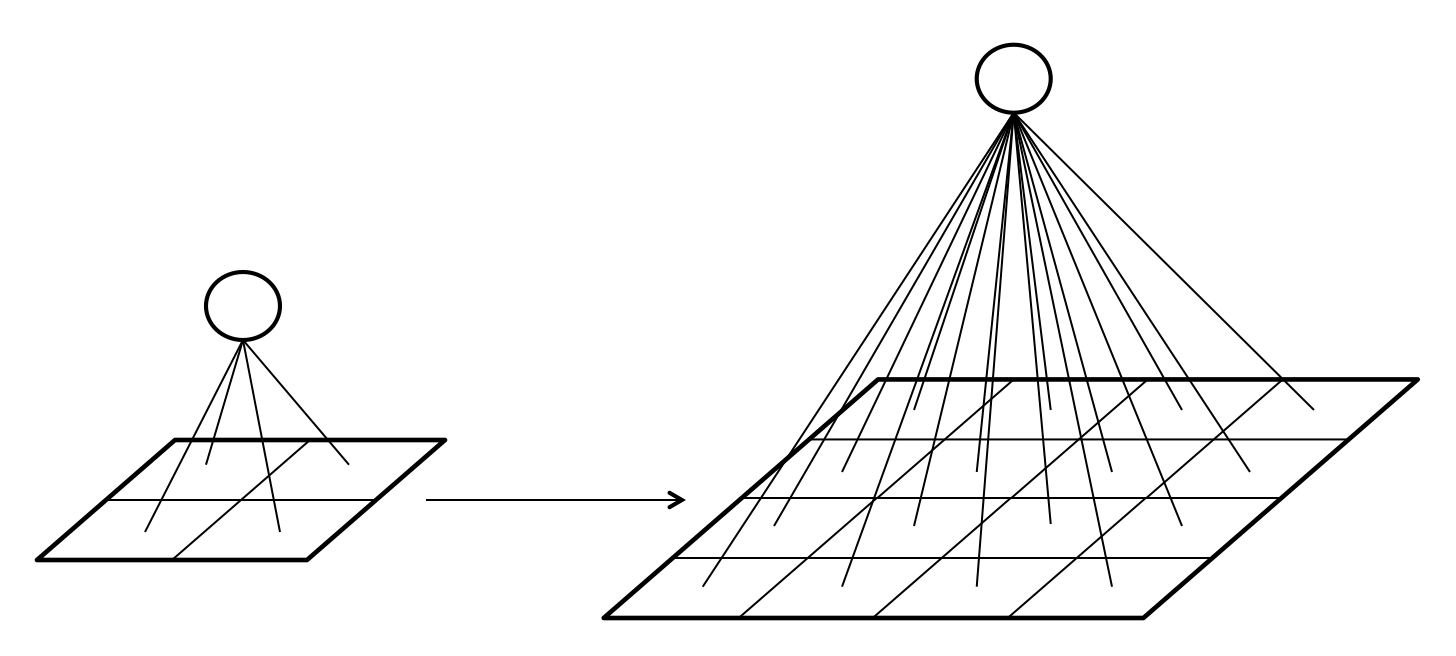
\includegraphics[scale=0.35]{mteorico/fc_dont_scale.png}
        \caption{La densidad de conexiones se incrementa según el tamaño de la imagen}
        \label{fig:fc_dont_scale}
        \source{Fundamentals of Deep Learning, \cite{dlBook}}
    \end{figure}

    Tomando como base el funcionamiento de la visión humana, capas de una red de convolución tienen neuronas dispuestas en tres dimensiones, por lo que las capas tienen una anchura, altura y profundidad, como se muestra en la Fig.~\ref{fig:convnet_scheme}. Como veremos, las neuronas de una capa única de convolución solo conectan a una región pequeña de la capa precedente, por lo que evitan el derroche de las neuronas totalmente conectadas. El proceso de una convolución puede expresarse fácilmente, procesa un volumen de información de 3 dimensiones para producir un nuevo volumen de 3 dimensiones \cite{dlBook}.
    \begin{figure}[htp]
        \centering
        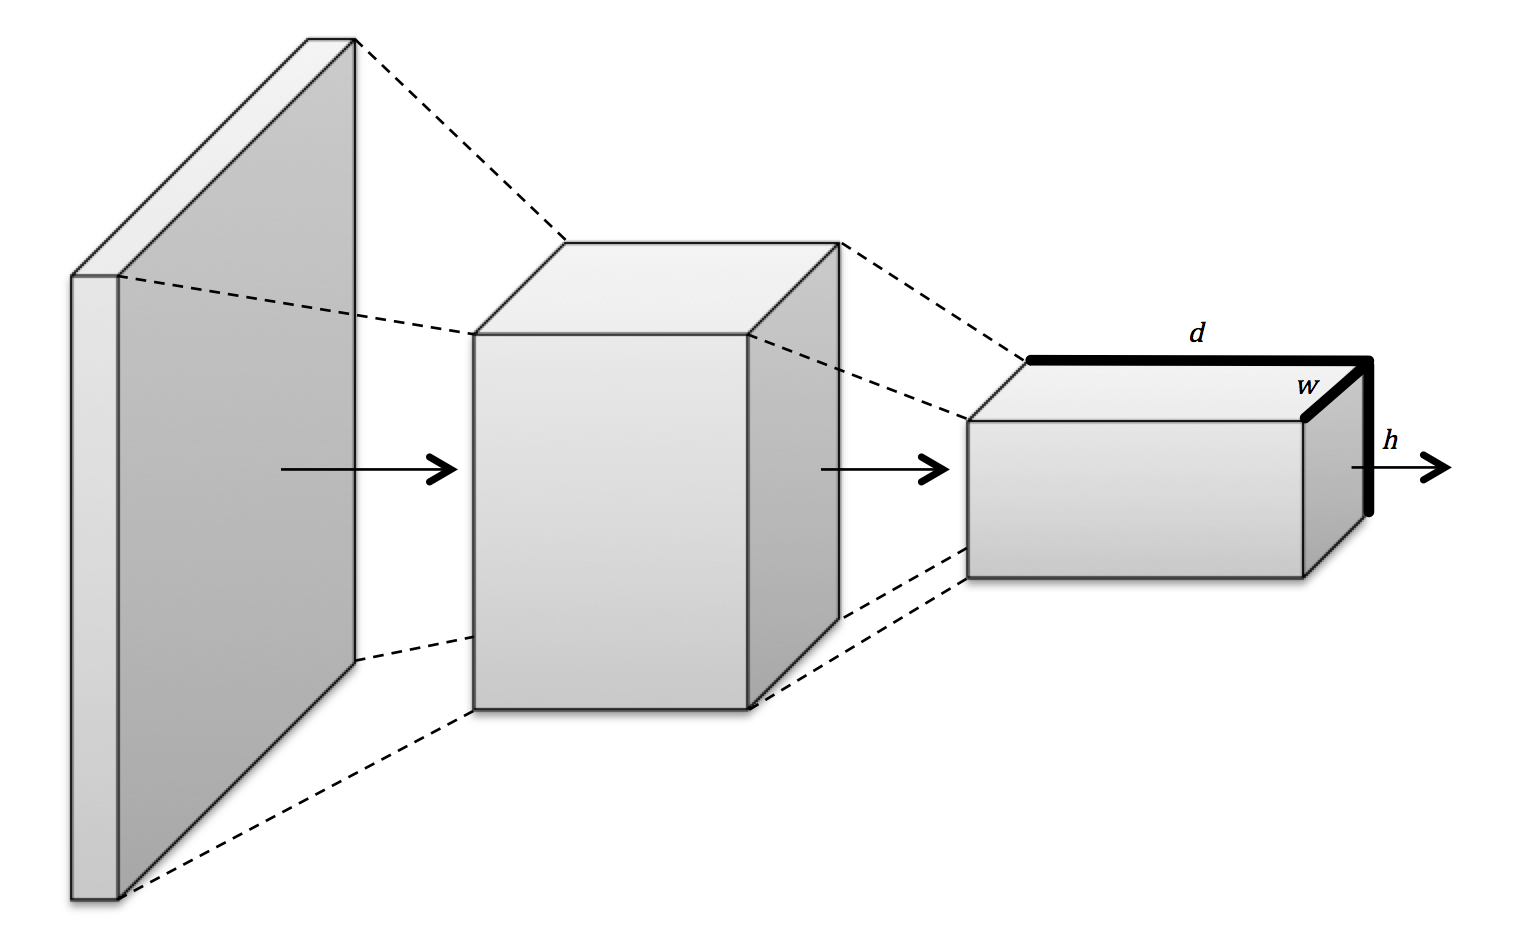
\includegraphics[scale=0.32]{mteorico/convnet_scheme.png}
        \caption{Capas de una red convolutiva}
        \label{fig:convnet_scheme}
        \source{Fundamentals of Deep Learning, \cite{dlBook}}
    \end{figure}

    Para entender el proceso de convolución debemos conocer el termino filtro, que es esencialmente un detector de característica, que para entender su funcionamiento, se considerar la Fig.~\ref{fig:image_no_filter}, \cite{dlBook}.
    \begin{figure}[htp]
        \centering
        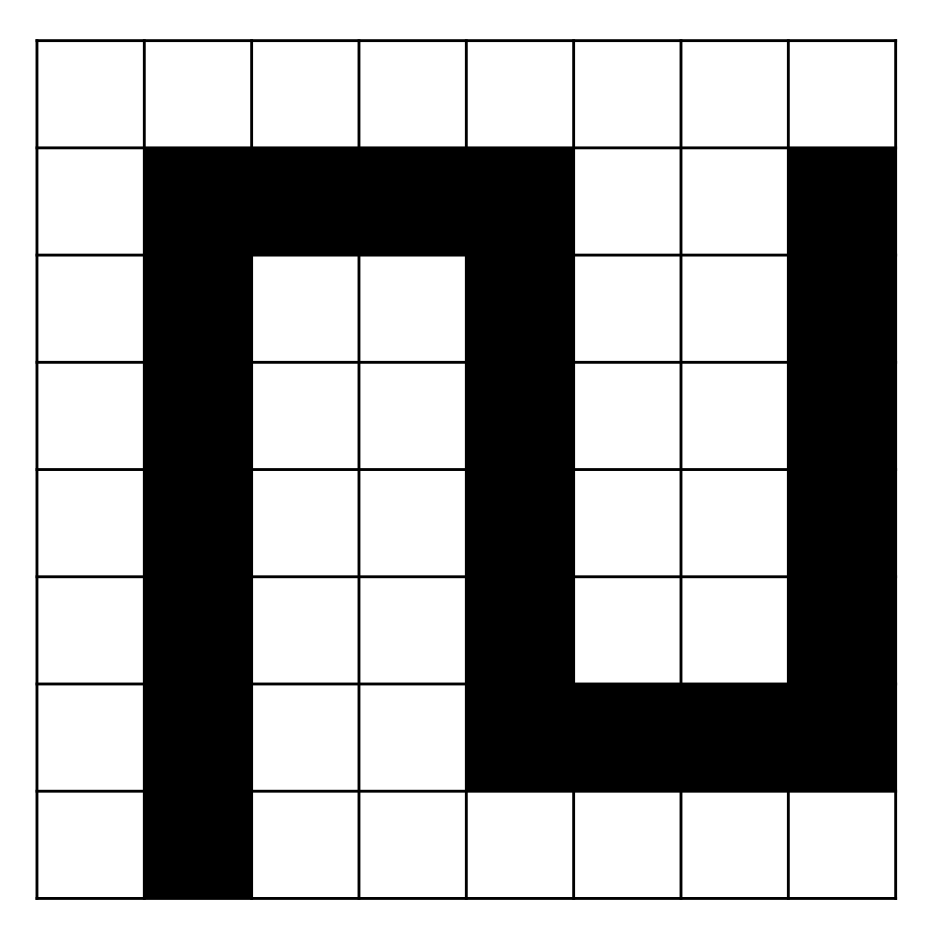
\includegraphics[scale=0.23]{mteorico/image_no_filter.png}
        \caption{Imagen en blanco y negro}
        \label{fig:image_no_filter}
        \source{Fundamentals of Deep Learning, \cite{dlBook}}
    \end{figure}

    Dado el caso que se requiera detectar líneas verticales y horizontales en una imagen. Una solución sería el uso de un detector de características, como se muestra en la Fig.~\ref{fig:image_two_filter}. Por ejemplo, para detectar líneas verticales, se puede utilizar el detector de característica de la parte superior de la imagen, es podría deslizarse a través de la totalidad de la imagen para verificar si existe alguna coincidencia, en la matriz de la parte superior derecha de la Fig.~\ref{fig:image_two_filter} se puede verificar el resultado, si hay una coincidencia se sombrea la casilla de negro y si no lo hay se deja en blanco. Este resultado es el mapa de características, que indica el lugar donde se han encontrado las característica que se buscaban en la imagen original. Se puede hacer el mismo tratamiento para el detector de línea horizontal (parte inferior de la imagen), dando como resultado el mapa de características de la esquina inferior derecha, \cite{NIPS2010_0550, dlBook}.
    \begin{figure}[htp]
        \centering
        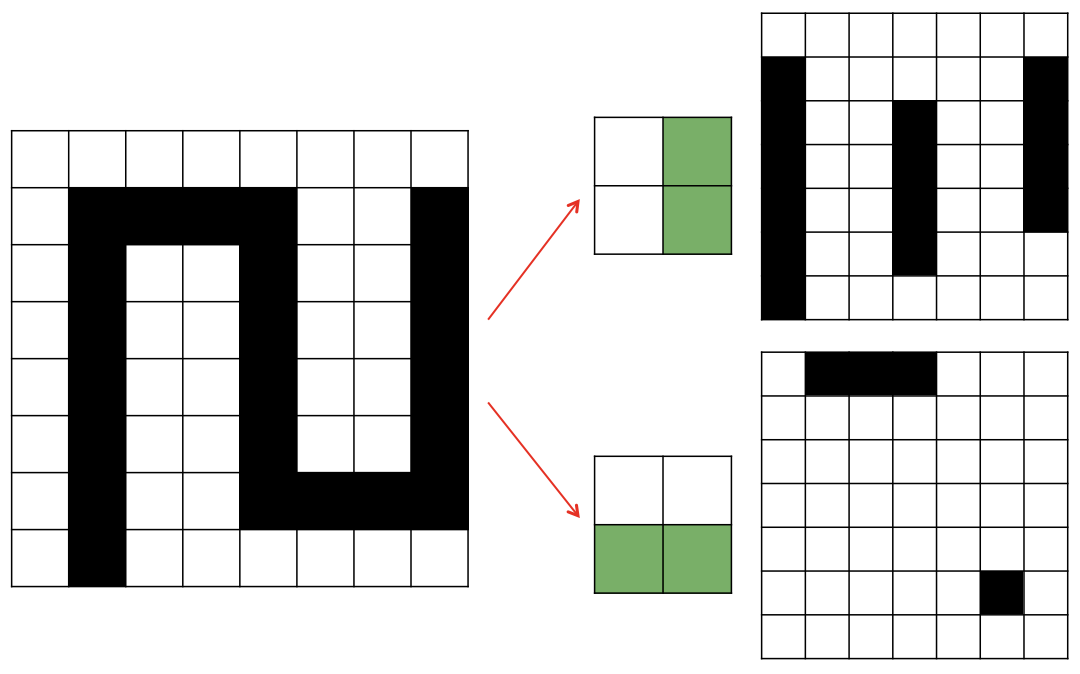
\includegraphics[scale=0.4]{mteorico/image_two_filter.png}
        \caption{Filtros para detectar lineas horizontales y verticales}
        \label{fig:image_two_filter}
        \source{Fundamentals of Deep Learning, \cite{dlBook}}
    \end{figure}

    Esta operación es llamada convolución, se toma un filtro para multiplicarlos sobre el área entera de una imagen de entrada. Los filtros representan distintas combinaciones de conexiones (se resalta una de estas combinaciones en la Fig.~\ref{fig:conv_neuron}), en esta figura las conexiones con las mismas tonalidades mantienen sus mismos pesos a través de todas las neuronas de entrada, se puede lograr esto mediante la inicialización de todas las conexiones en un grupo con pesos idénticos y siempre corrigiendo los pequeños cambios de peso, la capa de salida es el mapa de características generado por este filtro \cite{dlBook}.
    \begin{figure}[htp]
        \centering
        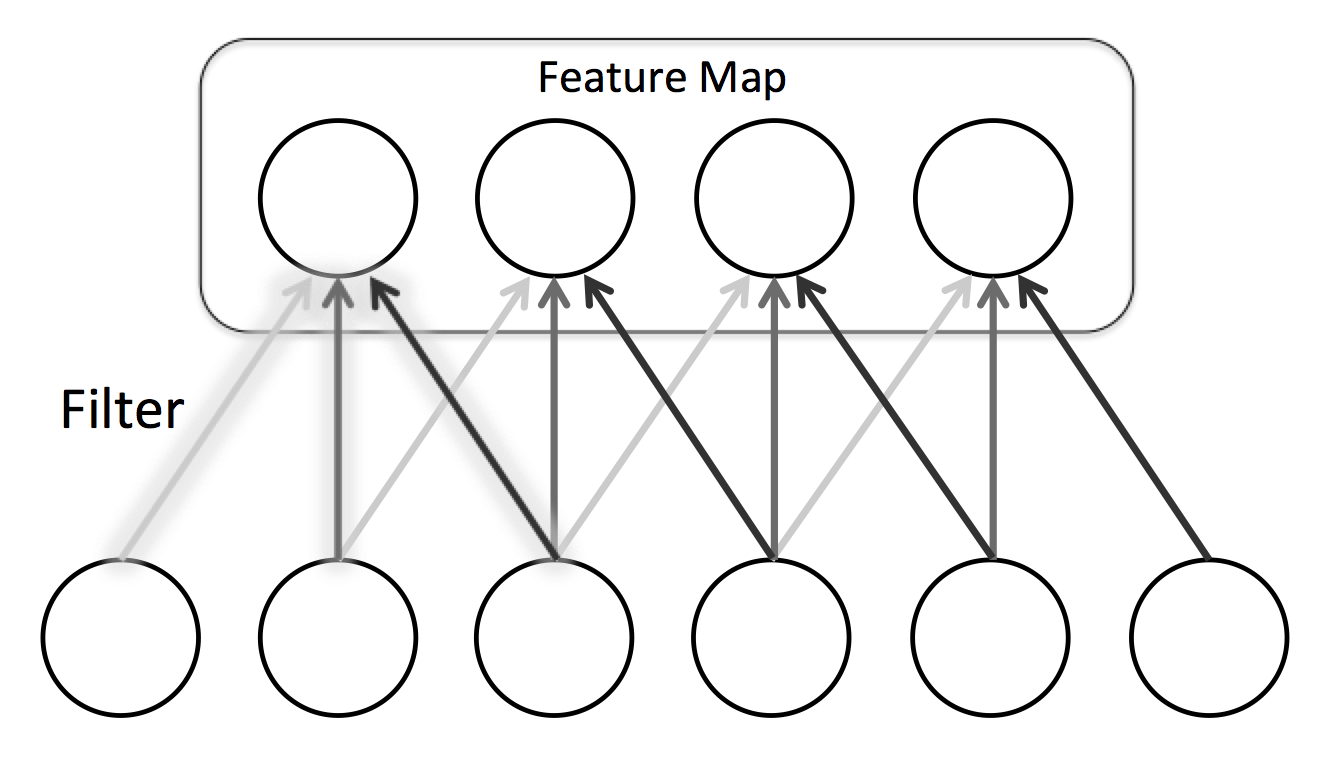
\includegraphics[scale=0.3]{mteorico/conv_neuron.png}
        \caption{Representación de un filtro y su mapa de características resultante}
        \label{fig:conv_neuron}
        \source{Fundamentals of Deep Learning, \cite{dlBook}}
    \end{figure}

    Matemáticamente se define a los $k^{th}$ mapas de características en la capa $m$ como $m^k$, por otra parte, se define un filtro correspondiente conformado por los valores de los pesos $W$, y se asume que las neuronas en el mapa de características tiene un \textit{bias} $b^k$ (el \textit{bias} se mantiene idéntico para todas las neuronas de un mapa de características). Entonces se puede expresar el mapa de características de la siguiente manera:

    \begin{equation}
		m^k_{ij}=f((W*x)_{ij}+b^k)
	\end{equation}
	
	En concreto, los filtros no sólo operan en un único mapa de características. Operan en todo el volumen de mapas de características que se han generado en una capa particular. Si se considera una situación en la que se desea detectar una cara en una capa particular de una red de convolución, y se han acumulado tres mapas de características, uno para los ojos, uno para la nariz, y uno para la boca. Para tomar tomar una decisión sobre la existencia de una cara, se debe combinar pruebas sobre múltiples mapas de características. Esto es igualmente necesario para una imagen de entrada con tres canales de color (RGB), por lo que requieren tres secciones en el volumen de entrada (una sección para cada canal). Como resultado, los mapas de características deben ser capaces de operar sobre los volúmenes de datos de 3 dimensiones (ancho, alto y profundidad). Esto se muestra a continuación en la Fig.~\ref{fig:color_conv}. Cada célula en el volumen de entrada es una neurona. Una porción local se multiplica con un filtro (que corresponde a los pesos en la capa de convolución) para producir una neurona en la siguiente capa volumétrica de las neuronas, \cite{dlBook}.
	\begin{figure}[htp]
        \centering
        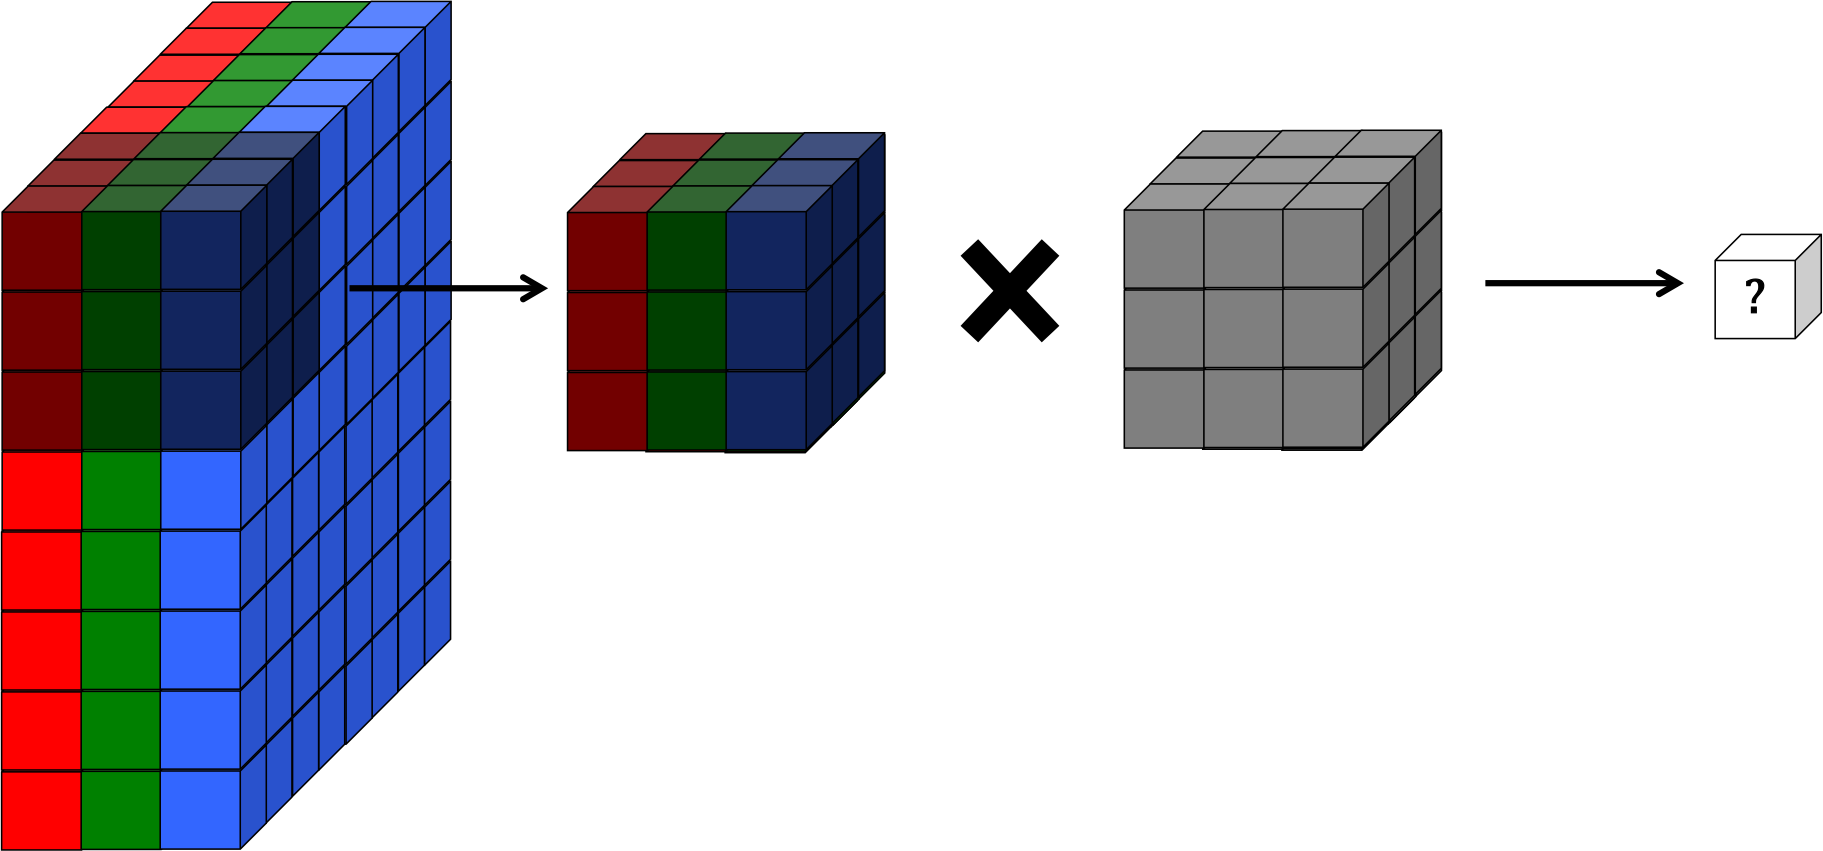
\includegraphics[scale=0.3]{mteorico/color_conv.png}
        \caption{Convolución de una imagen a color RGB}
        \label{fig:color_conv}
        \source{Fundamentals of Deep Learning, \cite{dlBook}}
    \end{figure}

	Como se ha observado anteriormente, una capa de convolución (que consiste en un conjunto de filtros) convierte un volumen de valores en otro volumen de valores. La profundidad del filtro corresponde a la profundidad del volumen de entrada. Esto es para que el filtro pueda combinar la información de todas las características que se han aprendido. La profundidad de el volumen de salida de una capa convolucional, equivalente al número de filtros en esa capa, debido a que cada filtro produce una porción del volumen de datos. Visualizamos estas relaciones en la Fig.~\ref{fig:conv_depth}
	\begin{figure}[htp]
        \centering
        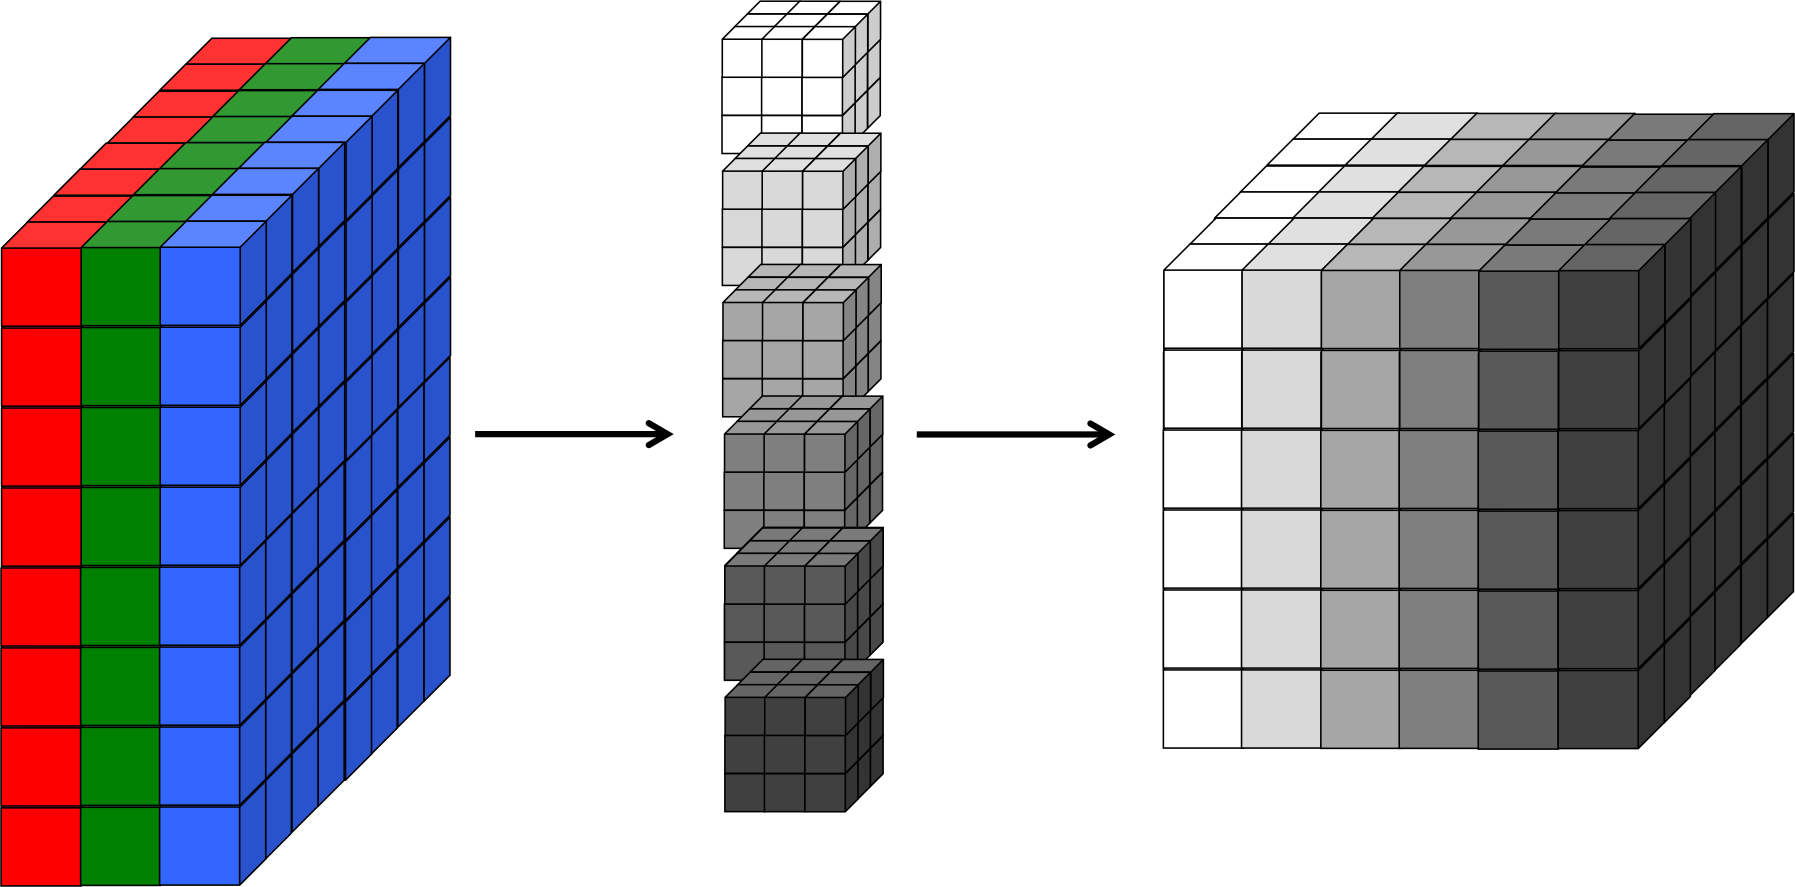
\includegraphics[scale=0.3]{mteorico/conv_depth.png}
        \caption{Visualización en 3d de una convolución}
        \label{fig:conv_depth}
        \source{Fundamentals of Deep Learning, \cite{dlBook}}
    \end{figure}


    \subsection{Agrupación Máxima o \textit{Max Pooling}}

    Para reducir la dimensionalidad de los mapas de características y afinar las características localizadas, a veces es necesario insertar una capa de agrupación máxima después de una capa de convolución. La idea esencial detrás de la agrupación máxima es dividir cada mapa de características en porciones de igual tamaño. Entonces se crea un mapa de características condensado, en concreto se define una celda que representa a toda una porción del mapa de características, calculando el valor máximo de la porción para propagar este valor máximo en la celda correspondiente del mapa de características condensado. Este proceso se ilustra en la Fig.~\ref{fig:max_pooling}, a continuación \cite{dlBook}:
	\begin{figure}[htp]
        \centering
        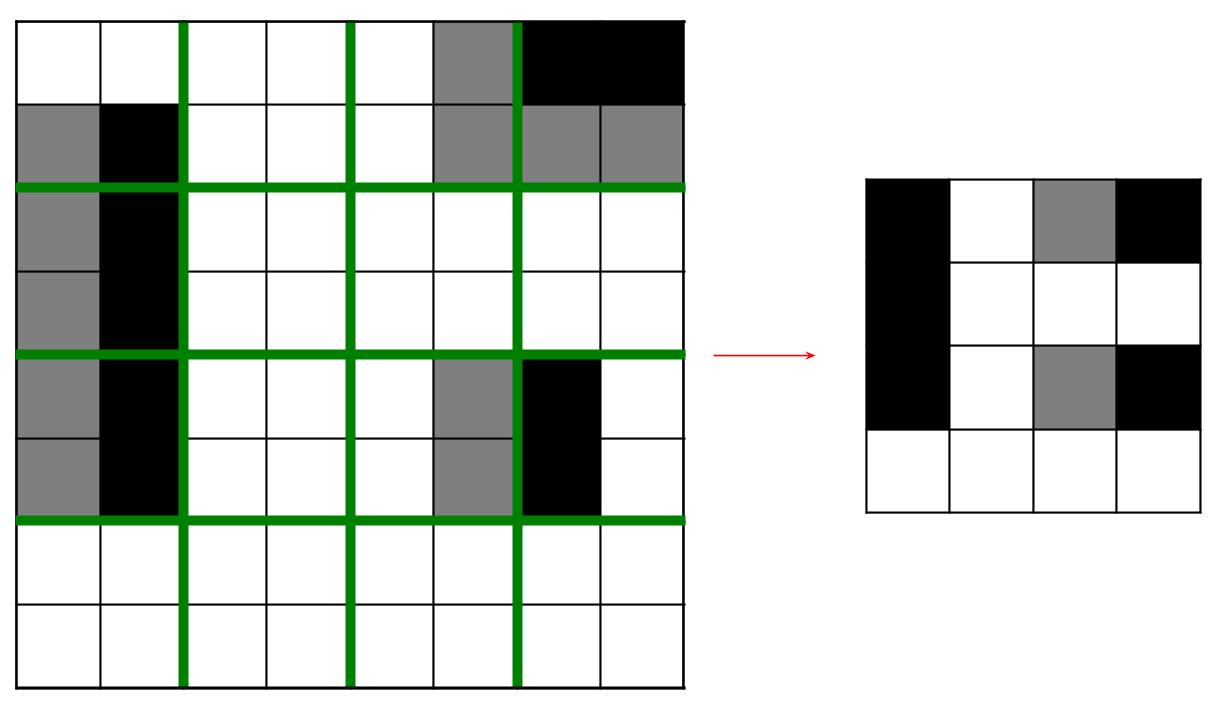
\includegraphics[scale=0.4]{mteorico/max_pooling.png}
        \caption{Reducción de parámetros utilizando agrupación máxima}
        \label{fig:max_pooling}
        \source{Fundamentals of Deep Learning, \cite{dlBook}}
    \end{figure}

    Podemos describir la capa de agrupación con dos parámetros, la dimensión de la ventana $e$ y el salto $s$. Es importante tener en cuenta que sólo se utilizan dos principales variaciones de la capa de agrupación. La primera es la capa que no existe solapamiento con $e=2$, $s=2$. La segunda es la capa con solapamiento, $e=3$, $s=2$. Las dimensiones resultantes de cada mapa de características son las siguientes:

    \begin{itemize}
		\item Ancho, $w_{out}=\left[\frac{w_{in}-e}{s}\right]+1$.
		\item Alto, $h_{out}=\left[\frac{h_{in}-e}{s}\right]+1$.
	\end{itemize}
	
	Una propiedad interesante de la agrupación máxima, es que es invariante a nivel local. Esto significa que incluso si las entradas cambian un poco, la salida de esta capa se mantiene constante. Esto tiene importantes implicaciones para los algoritmos visuales, la invariancia local es una propiedad útil para las características que están siempre presentes en un mismo lugar. Sin embargo, obtener grandes cantidades de invariancias locales puede destruir la capacidad de la red para almacenar información importante. Por eso es recomendable mantener pequeña la dimensión de la ventana de agrupación $e$, \cite{dlBook}.
	

\section{Auto-codificadores}

    %La flexibilidad de cambio de las redes neuronales es una propiedad muy útil. Esta capacidad de cambio conduce a grandes mejoras en la precisión, en comparación con modelos básicos de aprendizaje de maquina. Una de la primeras mejoras realizadas en el aprendizaje profundo fue el pre-entrenamiento de redes profundas. Este enfoque se basa en la observación de que la inicialización aleatoria es una mala idea, y que pre-entrenar cada capa con un algoritmo de aprendizaje no supervisado puede permitir mejores pesos iniciales \cite{Le15atutorial}.
    Los auto-codificadores pertenecen a una clase de algoritmos de aprendizaje conocidos como aprendizaje no supervisado. A diferencia de los algoritmos supervisadas, los algoritmos de aprendizaje sin supervisión no necesitan información de la etiqueta para los datos. En otras palabras, nuestros datos sólo tienen de $x(i)$, pero no tienen los $y(i)$, que vendrían a ser la etiquetas de los datos \cite{Le15atutorial, website:UFLDL}. Un auto-codificador es una técnica muy utilizada en el aprendizaje no supervisado, aunque también haya sido utilizada de distintas maneras y con distintos objetivos.

    \subsection{Compresión de data}

    En \cite{Le15atutorial}, se considera el siguiente ejemplo, se desea desarrollar un programa para enviar algunos datos del teléfono móvil a la nube. Para limitar el uso de la red, se debe optimizar cada \textit{bit} de datos que vamos a enviar. Los datos son una colección de puntos, cada uno tiene dos dimensiones, como se ve en la Fig.~\ref{fig:aenco1}
    \begin{figure}[htp]
        \centering
        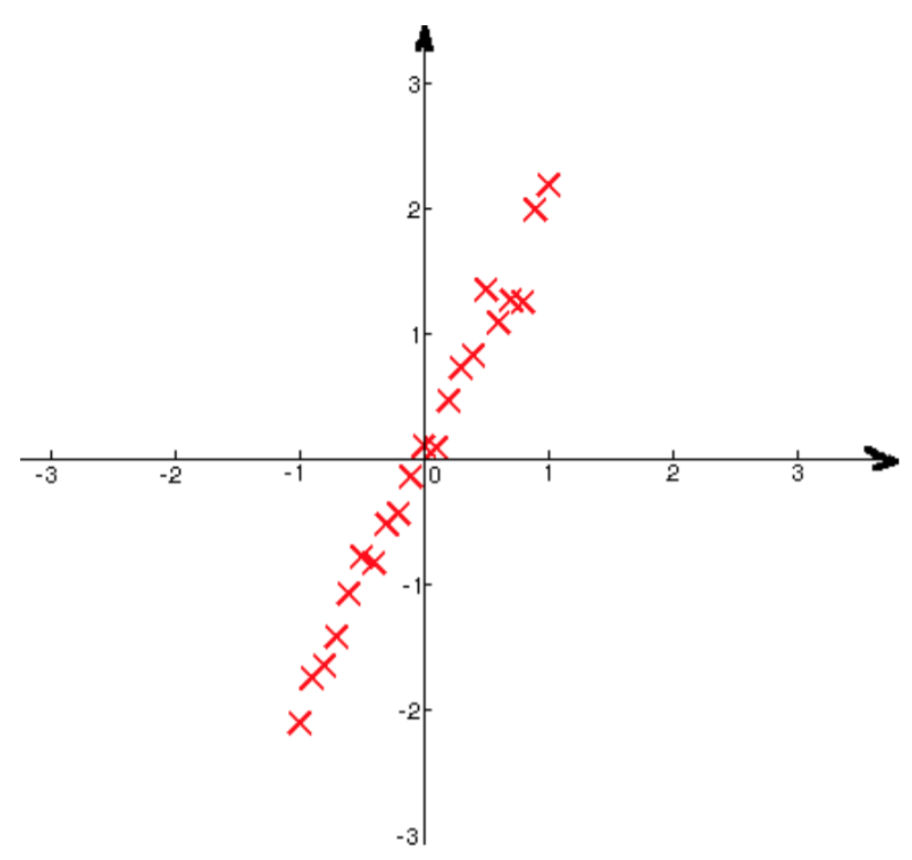
\includegraphics[scale=0.37]{mteorico/aenco1.png}
        \caption{Puntos en un plano 2d}
        \label{fig:aenco1}
        \source{\cite{Le15atutorial}}
    \end{figure}

    En la Fig.~\ref{fig:aenco1}, las cruces rojas son los puntos de datos, el eje horizontal es el valor de la primera dimensión y el eje vertical es el valor de la segunda dimensión. Tras la visualización, notamos que el valor de la segunda dimensión es aproximadamente el doble que de la primera dimensión. Teniendo en cuenta esta observación, se puede enviar sólo la primera dimensión de cada punto de datos a la nube. Luego, en la nube, solo se necesita calcular el valor de la segunda dimensión, duplicando el valor de la primera dimensión. La compresión es con perdida, pero reduce el tráfico de red en un 50\%. Ya que el tráfico de red es lo que tratamos de optimizar, esta idea parece razonable \cite{Le15atutorial}.
    \\\\
    El objetivo de los auto-codificadores es poder resolver el ejemplo anterior de manera sistemática. Formalmente, suponemos que tenemos un conjunto de puntos de datos $\{x(1), x(2),$ $..., x(m)\}$, donde cada punto de datos tiene varias dimensiones. La pregunta es si hay una manera general de asignarlos a algún conjuntos de datos $\{z(1), z(2), ..., z(m)\}$, donde $z$ tiene una dimensión menor a $x$ y los $z(i)$ pueden fielmente reconstruir las $x(i)$. Para responder a esto, se nota que en el ejemplo anterior, para enviar datos desde el teléfono celular a la nube, tiene tres pasos:

    \begin{itemize}
        \item Codificación: Desde el celular. se asigna la data $x(i)$ comprimida a $z(i)$.
        \item Envío: Se envía $z(i)$ a la nube.
        \item Decodificación: En la nube, se asigna desde la data comprimida $z(i)$ a $\tilde{x}(i)$, que es una aproximación de $x(i)$.
    \end{itemize}

    Para asignar los datos de un lado a otro de manera sistemática, definimos que $z$ y $\tilde{x}$ son funciones de entrada, de la siguiente manera:

    \begin{equation}
        z{(i)} =W_1x{(i)} + b_1
    \end{equation}
    \begin{equation}
        \tilde{x}{(i)} =W_1z{(i)} + b_1
    \end{equation}

    Si $x(i)$ es un vector de dos dimensiones, puede ser posible visualizar los datos para encontrar $W1, W2, b_1, b_2$ analíticamente, donde $W1, W2$ son matrices bidimensionales de pesos y $b_1, b_2$ son el componente \textit{bias}. En casos prácticos, es difícil encontrar esas matrices usando la visualización, por lo que es necesario utilizar el gradiente descendente \cite{stochastic-gradient-tricks}. La meta es tener un $\tilde{x}(i)$ aproximado a $x(i)$, para esto se establece la siguiente función objetivo, que es la suma de diferencia de cuadrados entre $\tilde{x}(i)$ y $x(i)$:
    \begin{equation}
    \begin{aligned}
     J(W_1,b_1,W_2,b_2) & = \sum_{i=1}^m\left(\ \tilde{x}(i)-x(i)\ \right )^{\ 2} \\
      & = \sum_{i=1}^m\left(\ W_2z(i) + b_2-x(i)\ \right )^{\ 2}\\
     & = \sum_{i=1}^m\left(\ W_2 \ (W_1x(i)+b_1) \ + b_2-x(i)\ \right )^{\ 2}
    \end{aligned}
    \end{equation}
    En la Fig.~\ref{fig:aenco2}, Se observa como se trata de comprimir datos de 4 dimensiones a 2 dimensiones utilizando una red neuronal con una capa oculta. La función de activación de la capa oculta es no lineal. Si los datos fueran altamente no lineales, se podría añadir más capas ocultas a la red para tener un auto-codificador profundo.
    \begin{figure}[htp]
        \centering
        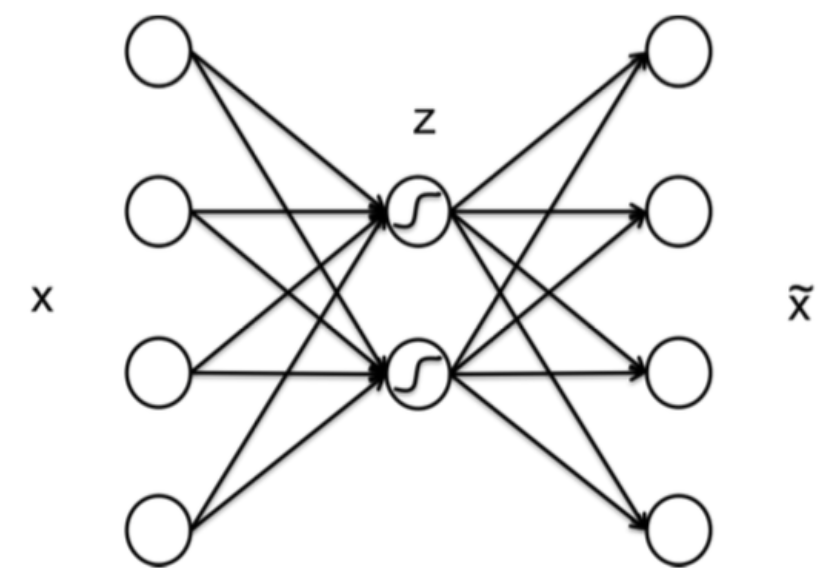
\includegraphics[scale=0.49]{mteorico/aenco2.png}
        \caption{Arquitectura de auto-codificador no lineal}
        \label{fig:aenco2}
        \source{\cite{Le15atutorial}}
    \end{figure}

  

\section{Consideraciones Finales}\label{sec:consideraciones-finales}

En este capítulo fue presentada una visión general sobre minería de series \mbox{temporales}, destacando la consulta por similitud y el descubrimiento de \textit{motifs}  que son tópicos de interés para este trabajo.

A pesar de las recientes investigaciones en algoritmos exactos, los algoritmos aproximados pueden ser la mejor opción en muchos dominios de aplicación debido a su eficiencia en tiempo y espacio. En esos dominios, el \textit{trade-off} entre tiempo de ejecución y precisión de la solución claramente se inclina para la primera. Este hecho es importante en las bases de la propuesta de este trabajo.

Además, fueron discutidas técnicas de representación y medidas de similitud en series temporales, que tienen como objetivo minimizar el ruido de los efectos de la alta dimensión en aplicaciones de minería de series temporales. Esto es importante, pues permite llevar en consideración la naturaleza de los datos en los métodos de minería.






%
\chapter{Teoría Fractal}
\hrule \bigskip \vspace*{1cm}

\section{Consideraciones Iniciales}

Un fractal es definido como un objeto que presenta aproximadamente las mismas características independientemente de la escala donde es analizada, es un objeto que se parece a si mismo. Por otro lado, las partes del fractal son similares, exactas o estadísticamente  al  fractal completo. Esto es, a una escala mejor los detalles son similar a las características de una escala mayor \cite{Schroeder:1991,traina2005using}.
 
Por ejemplo, el triangulo $Sierpinkski$ es un fractal geométrico, que ha sido construido en un proceso iterativo, teóricamente infinito.  En un triangulo equilátero ABC, donde primero se ha removido el triangulo central A', B', C',  de cada uno de los tres triángulos restantes cuyos lados longitud igual a la mitad del lado de ABC, retiramos de nuevo el triángulo central. La figura \ref{fig:ima1} muestra los pasos iniciales del proceso de construcción de un triángulo de $Sierpinski$. El triángulo restante tiene ``agujeros'' independientes de la escala y cada triángulo dentro de la primera es una ``miniatura'' de todo el triángulo.
\begin{figure}[h]
\centering
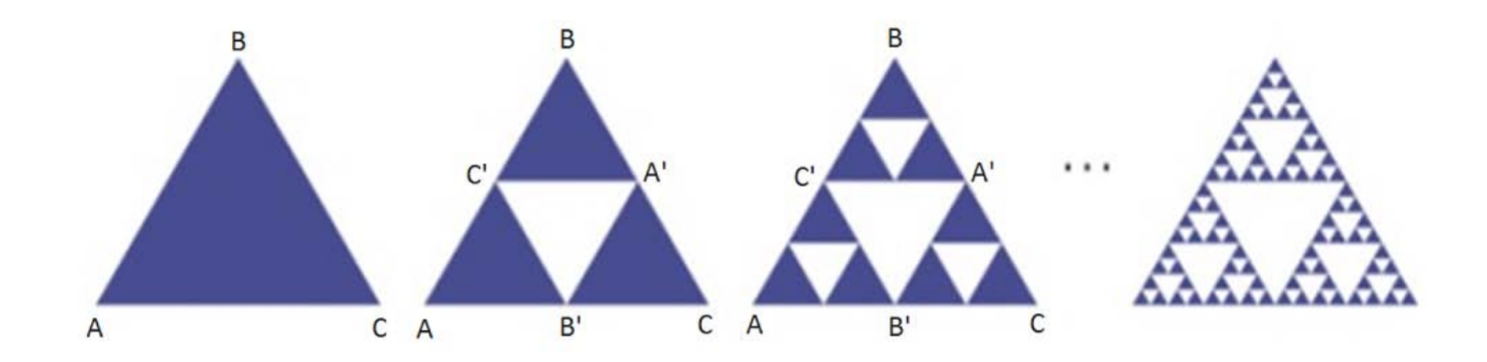
\includegraphics[scale=0.75]{chapter4/ima1.png}
\caption{Pasos del proceso de construcción del triangulo de $Sierpinsky$}
\label{fig:ima1}
\end{figure}
Hay muchas otras estructuras matemáticas definidas como fractal, como las curvas de   $Koch$,  el conjunto de $Cantor$ y el conjunto de $Mandelbrot$ que son presentados en la figura \ref{fig:ima2}. Son también ejemplos de fractales en la naturaleza, por ejemplo: nubes, montañas, hortalizas, árboles, La costa de continentes, islas entre otros.
\begin{figure}[h]
\centering
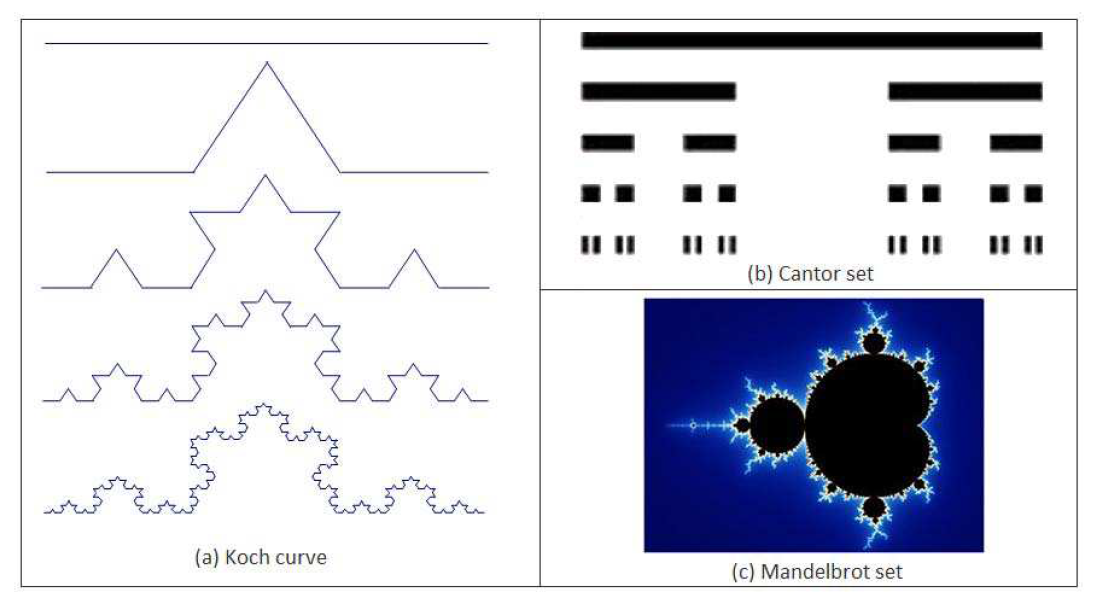
\includegraphics[scale=1.2]{chapter4/ima2.png}
\caption{Algunos ejemplos de fractales (a y b) fractales geométricos y (c) fractales algebraicos}
\label{fig:ima2}
\end{figure}


Los conceptos de fractal se han aplicado a varias tareas en el análisis de datos y la minería de datos. Una de ellas es la estimación de la dimensión intrínseca (D) de un conjunto de datos, que es relacionado  con el concepto de dimensión embebida (E) \cite{conf/pods/FaloutsosK94}.
\\\\
\textbf{Definición 3.1 Dimensión embebida  E:} Dado un conjunto finito de datos $A$, la  
dimensión embebida $E \in N$ es el número de atributos que definen $A$. Es decir, $E$ es la dimensión de el espacio en el que se encaja el conjunto de datos.
\\\\
\textbf{Definición 3.2 Dimensión intrínseca D:} Dado un conjunto de datos finitos $A$, su dimensión intrínseca
$D \in R^+$, es la dimensionalidad del objeto representado por los datos, independientemente de la
dimensión del espacio en el que está embebido.
\\\\
La dimensión intrínseca (D) es una medida de la cantidad de información que el conjunto de datos representa. Por ejemplo, la dimensión intrínseca de un conjunto de puntos distribuidos a lo largo de una linea  es igual a uno; si el conjunto está embebido  en un espacio dimensional superior, la dimensionalidad intrínseca   continúa igual a uno tal como se ilustra en la Figura \ref{fig:ima3}.

\begin{figure}[h]
\centering
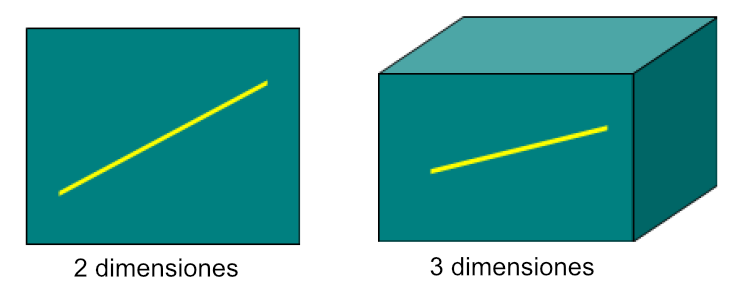
\includegraphics[scale=1.2]{chapter4/ima3.png}
\caption{Una linea embebida en dos o tres dimensiones donde $D=1$.}
\label{fig:ima3}
\end{figure}


Faloutsos & Kamel (1994) \cite{conf/pods/FaloutsosK94} propusieron el uso de la dimensión intrínseca como una herramienta para medir el comportamiento no uniforme de conjuntos de datos reales. Además, los autores presentaron estudios empíricos para demostrar que los datos reales suelen tener un comportamiento de auto-similitud, que es  una   característica fundamental de los objetos fractales. Por lo tanto, la dimensión intrínseca $D$ de un conjunto de datos real puede calcularse usando la dimensión fractal.

La dimensión intrínseca basada en la dimensión fractal ha sido empleada como una herramienta para el análisis de agrupamiento \cite{Barbara2003},  reglas de asociación temporal \cite{Barbara2004}, selección de atributos \cite{journals/jidm/TrainaTF10}, series cronológicas \cite{Chakrabarti:2002:FLA:584792.584797} y la minería de datos espaciales \cite{Traina:2001:TST:502512.502538}.

En este capítulo presentamos los principales conceptos relacionados con la teoría fractal que son usados en algunos de los métodos propuestos en esta tesis. La sección 2 muestra diferentes maneras de Calcular la dimensión fractal. El cálculo de correlación indicado por la correlación por la dimensión fractal se detalla en la Sección 3. La teoría fractal empleada para analizar   datos en la sección 3.

\section{Dimensión fractal}

Los fractales suelen tener características inusuales que pueden considerarse paradojas. Por ejemplo, el triángulo de $Sierpinski$ tiene un perímetro infinito (proporcional a $lim_{i\rightarrow\infty} (1+1/2)^i  $ ) y nulo (proporcional a $lim_{i\rightarrow\infty} (3/4)^i $) ya que a cada iteración de su proceso de construcción, que  teóricamente  es infinito, su perímetro aumenta y su área disminuye. Debido a estas propiedades, este fractal no puede ser considerado un objeto euclidiano unidimensional  (ya que su perímetro no es finito) ni un objeto euclidiano bidimensional (puesto que su área es nula). Así, es posible considerar una dimensionalidad de fraccionamiento llamada fractal \cite{di2016fractal}. Intuitivamente, la dimensión fractal del triángulo de $Sierpinski$ esta entre un valor de 1 y 2. Matemáticamente, el valor preciso es 1,58.

Hay varias definiciones para la dimensión fractal, que se presentan brevemente en este sección. La medida básica de la dimensión fractal se dedica a los fractales denominados exactamente auto-similares. Este tipo de fractal se compone de $M$ réplicas que son   una  versión reducida $1:s$ del fractal original.

\textbf{Definición 3.3 Dimensión fractal D:} Sea $M$ el número de réplicas y $s$ el factor de  escala
 por el que se reduce cada réplica, la dimensión fractal D de un fractal auto-similar es   definido en un espacio E-dimensional como:

\begin{equation}
D \equiv \frac{log M}{log s}
\label{eq:ec1}
\end{equation}

El triángulo de $Sierpinski$, por ejemplo, es un fractal exactamente auto-similar, porque su regla de construcción genera tres réplicas en escala $1:2$ en cada iteración. Por lo tanto, la dimensión fractal de $Sierpinski$ es $D = \frac{log 3}{log 2} \approx 1.58$. Similarmente, en la Figura \ref{fig:ima2}
el conjunto de Cantor conjunto y la curva de Koch son  fractales auto-similares con la dimensión fractal $ D = \frac{log2}{log3} \approx 0.63$ y $ D = \frac{log4}{log3} \approx 1.26$ respectivamente.

Esta definición de la dimensión fractal D es adecuada para Fractales  auto-similares matemáticamente  exactos. Sin embargo, para conjuntos de datos llamados  Fractales auto-similares estadísticamente, que no tienen reglas de construcción bien definidas, es más apropiado  calcular la dimensión fractal mediante el método de recuento de cajas (box-counting) \cite{Schroeder:1991}, que define la Correlación de Dimensión Fractal   $D_2$ tal como se presenta en Ecuación \ref{eq:ec2}

\textbf{Definición 3.4 Correlación de Dimensión Fractal $D_2$:} Dado un conjunto de datos auto-similar en el rango de escalas $[r1, r2]$, su dimensión fractal de correlación $D_2 \rightarrow \left[ \mathbb{R}^{+} \right]$ se mide como

\begin{equation}
D_2 \equiv  \frac{\partial log (\sum_i C_{r,1}^2)}{\partial (r)} \qquad \:r \epsilon [r1,r2 ]
\label{eq:ec2}
\end{equation}
donde $r$ es el lado de las celdas en una (hiper) cuadrícula  que divide el espacio del  conjunto de datos, y $C_r,i$, es el recuento de puntos en la i-ésima celda.

De forma práctica, el valor derivado que define la dimensión fractal $D_2$ puede se obtiene mediante la construcción de la gráfica de recuento de bloques, que representa los valores de $\sum_i C_{r,1}^2$  y $log (r)$ en un gráfico. Para los conjuntos fractales, la curva resultante es lineal en un intervalo $(r1, r2)$ y la dimensión fractal $D_2$ se estima por la pendiente de la línea que mejor se ajusta al intervalo analizado.

La figura \ref{fig:ima4} muestra un conjunto de $6561$ puntos en el triangulo de $Sierpinski$  y la gráfico en la escala log-log de la suma de la ocupación cuadrada $\sum_i C_{r,1}^2$ contra el tamaño de la celda  (radio) $r$.

\begin{figure}[h]
\centering
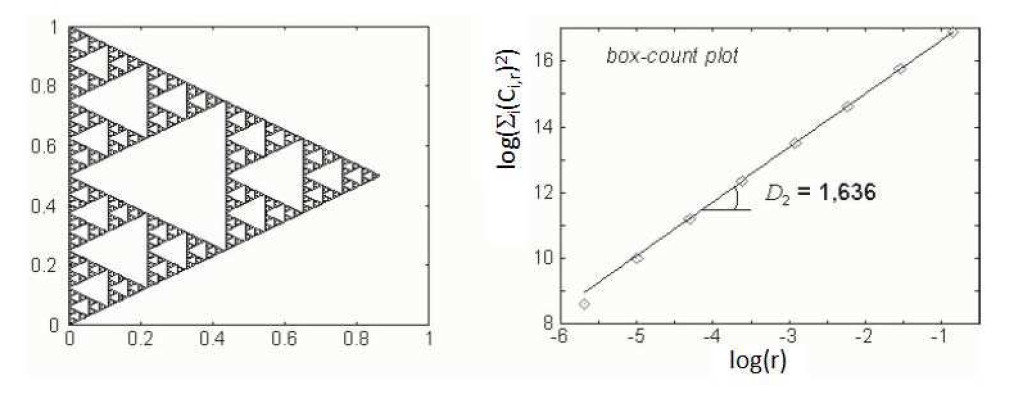
\includegraphics[scale=1.4]{chapter4/ima4.png}
\caption{El gráfico de conteo de cajas para el triangulo de $Sierpinki$.}
\label{fig:ima4}
\end{figure}

La dimensión fractal fue calculada por el algoritmo Liboc () (coste lineal respecto al número de elementos en el conjunto de datos)  \cite{DBLP:journals/jidm/TrainaTF10}.


\section{Algoritmo de Calculo de la Dimension Fractal}

Esta sección presenta un algoritmo para calcular la dimensión fractal D de cualquier conjunto dado de puntos en cualquier espacio E-dimensional. Una manera práctica de estimar D a partir de un conjunto de datos espaciales está utilizando el método de "recuento de cajas" [Schroeder 1991] \cite{schroeder}. Teóricamente, este método da una aproximación cercana a la dimensión fractal, y nuestros experimentos mostraron que efectivamente [Traina Jr. et al. 2000; 1999a] \cite{traina2000} \cite{traina1999}. Uno de los mejores algoritmos publicados para calcular D de un conjunto de datos es un algoritmo O (N log (N)), donde N es el número de puntos en el conjunto de datos [Belussi y Faloutsos 1995]\cite{belussi}. \\

Sin embargo, hemos desarrollado un nuevo, muy rápido, O (N) algoritmo para su implementación, que se presenta a continuación. Considere el espacio de direcciones de un conjunto de puntos en un espacio E-dimensional e imponga una E-rejilla con cuadrículas de tamaño de lado r. Centrándose en la i-ésima célula, sea $C r, i$ el recuento ('ocupaciones') de los puntos 2 en cada celda. Luego, calcule el valor $S (r) = i C r, i$. La dimensión fractal es la derivada de log $(S (r))$ con respecto al logaritmo del radio. \\

Al asumir conjuntos de datos auto-similares, esperamos que esta derivada resulte en un valor constante. Así, podemos obtener la dimensión fractal D de un conjunto de datos que traza $S (r)$ en escalas log-log para diferentes valores del radio r, y calcular la pendiente de la línea resultante. Es necesario procesar $S (r)$ para una cantidad R de valores de r, por lo que podemos lograr una aproximación estadística adecuada de la recta. Para evitar la lectura del conjunto de datos de nuevo para cada valor del radio, proponemos crear una estructura de cuadrícula de niveles múltiples, donde cada nivel tiene un radio de la mitad del tamaño del nivel anterior $(r = 1, 1/2, 1 / 4, 1/8, etc.)$. Cada nivel de la estructura corresponde a un radio diferente, por lo que la profundidad de la estructura es igual al número de puntos en el gráfico resultante. \\

La estructura se crea en la memoria principal, por lo que el número de puntos en el gráfico está limitado por la cantidad de memoria principal disponible. Si este gráfico es lineal para un rango adecuado de radios, el conjunto de datos es un fractal y su dimensión fractal D es la pendiente de la línea de ajuste de este gráfico. El algoritmo propuesto es lineal en el número de puntos en el conjunto de datos. La complejidad computacional del algoritmo es $O (N * E * R)$, donde N es el número de objetos en el conjunto de datos, E es la dimensionalidad de inclusión y R es el número de puntos utilizados para representar la función $S (r)$. Esto muestra que el algoritmo es escalable a conjuntos de datos de cualquier tamaño.\\

Para cada lado de celda dado r, sólo se mantienen las celdas que tienen al menos un punto ya procesado, contando la suma de ocupaciones $C r, i $ de esta celda. De esta manera, cada nuevo punto está directamente asociado a una célula en cada nivel, sin necesidad de ser comparado con los puntos de lectura anteriores. La figura 2 muestra la estructura utilizada en el algoritmo para conjuntos de datos bidimensionales y tridimensionales.\\

El lado de celda más grande del espacio de puntos genera $2 n$ células. En el siguiente nivel, cada célula se divide en otras 2 n células, y así sucesivamente. Dado que siempre se conoce la posición de cada célula en el espacio, cada célula está representada por: la suma de ocupaciones $C r, i$ en esta celda, y los punteros a las celdas en el siguiente nivel cubierto por esta celda (véase la Figura 2 ). Esta estructura es una especie de multi-dimensional "quad-árbol" (oct-tree para un espacio 3D, o E-dim-árbol). La Figura 3 muestra un ejemplo de esta estructura para un conjunto de datos con cinco puntos en tres niveles en un espacio bidimensional.\\


\begin{figure}[h]
\centering
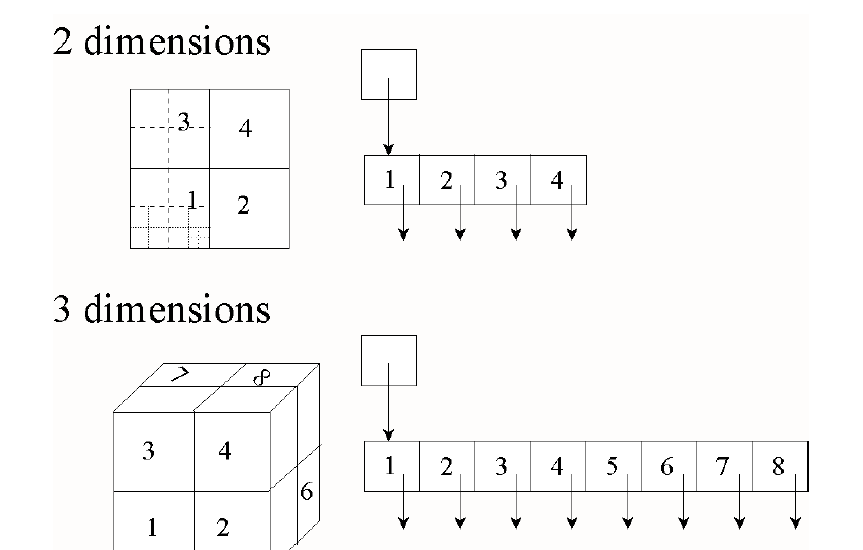
\includegraphics[scale=1.0]{chapter4/ima5.png}
\caption{ Representación de celdas de cuadrícula en espacios de 2 y 3 dimensiones. }
\label{fig:ima5}
\end{figure}
\\\\

Observe que se agregan nuevas celdas a la estructura cuando se solicita. Así, sólo se crean células ocupadas por al menos un punto $(C r, i> 0)$. El algoritmo procesa los puntos establecidos sólo una vez, por lo que es realmente muy rápido. El algoritmo 1 resume este proceso de cálculo.\\


\begin{figure}[h]
\centering
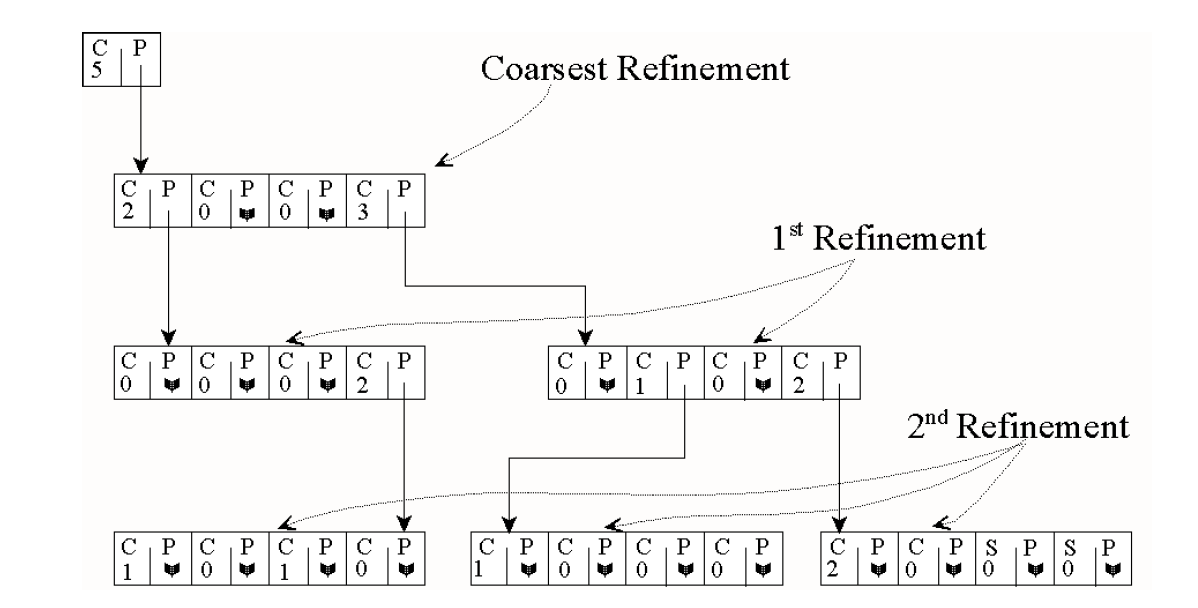
\includegraphics[scale=1.2]{chapter4/ima6.png}
\caption{Ejemplo de la estructura de datos utilizada para calcular la Suma de Ocupaciones de un conjunto de datos con 5 puntos (con tres niveles de resolución) }
\label{fig:ima6}
\end{figure}
 

\\\\
Observe que se agregan nuevas celdas a la estructura bajo demanda. Así, sólo las células ocupadas
Por al menos un punto $(C_{r,i}> 0)$. El algoritmo procesa sólo los puntos establecidos
Una vez, por lo que es realmente muy rápido. El algoritmo \ref{alg:algo1} resume este proceso de cálculo.
\\\\
\begin{algorithm}
\begin{algorithmic}[1]
\REQUIRE Normalizar el Dataset A(N filas, con E dimensiones/cada atributo)
\label{lin:lineaRara}
\ENSURE  Dimension fractal D
\FOR{Cada tamaño de grid deseaada $r = 1/2^j , j = 1,2, ...,l$}

    \FOR{Cada punto en el dataset}
    \STATE Decide cual celda del grid cae en (la i-esima celda)
    \STATE Incrementa la cuenta $C_i$
    \ENDFOR
    \STATE Procesa la sumatoria de los ocupados $S(r) = \sum C_i^2$
\ENDFOR

\STATE Imprime los valores de $log(r)$ y $log(S(r))$ generando un gráfico

\STATE Retorna la parte linear del gráfico cuesta abajo(regresión linear) de las dimensiones fractales D del dataset A

\end{algorithmic}
\caption{Procesar la dimensión fractal D del dataset A(conteo de cajas aproximadas)}
\label{alg:algo1}
\end{algorithm}
 
A medida que aumenta el lado de la cuadrícula, también aumenta el número de punteros a celdas vacías. Por lo tanto, para los conjuntos de datos de alta dimensión vale la pena mantener las celdas como listas enlazadas en lugar de arrays. Implementamos esta estructura como un objeto en C ++, usando una matriz para conjuntos de datos con la dimensión de incrustación menos o igual a tres, y usando una lista vinculada para conjuntos de datos con mayor dimensionalidad.	\\

%\chapter{Optimizaci\'on de la representaci\'on de datos}
 





 
%\chapter{Deep Fractal based Hashing - DAsH}
 {\textit{Este capítulo describe nuestra propuesta llamado \textit{Deep Fractal based  Hashing} (DAsH) diseñado para realizar una búsqueda aproximada escalable mediante un esquema de \textit{hashing} supervisado. }}
 
 

\section{Consideraciones Iniciales}

\initial{S}e han propuesto   algoritmos de búsqueda  kNN aproximada basados en hashing para operaciones de búsqueda en conjuntos de datos de alta dimensionalidad debido a su alto desempeño  en  recuperación y bajo costo de almacenamiento. Estudios recientes, promueven el uso de la Red Neural Convolucional (CNN) con técnicas de hashing para mejorar la precisión de búsqueda. Sin embargo, existen retos a resolver para encontrar una solución práctica y eficiente para indexar las características de la CNN, tales como la necesidad de un intenso proceso de entrenamiento para lograr resultados precisos  y la dependencia crítica de los parámetros de datos. 


En \textit{Machine Learning} las imágenes se describen a menudo mediante las características visuales manuales.  Sin embargo, estas características manuales no pueden revelar el significado semántico de alto nivel (etiquetas o tags) de las imágenes, y a menudo limitan el rendimiento de la recuperación de imágenes \cite{Li:2015:RSS:2881665.2882186}. Así, para obtener esta información semántica tenemos que trabajar con la información de la etiqueta y procesar los datos en un modo supervisado. Inspirado por recientes avances en \acf{CNN} para problemas de clasificación de imágenes, detección de objetos, y muchas otras tareas de visión \cite{ImageNet,NIPS2013_5207,LiuWJJC12}, muchos métodos resolvieron el problema de la precisión de la recuperación de similitud utilizando CNN como extractor de características y luego construir un código hash compacto de preservación de similitud para la recuperación rápida de imágenes.   De nuevo, \textit{hashing} es ampliamente usado para recuperar imágenes a gran escala así como las búsquedas de video y documentos porque la representación compacta del código hash es esencial para el almacenamiento de datos y es razonable para las búsquedas de consultas \cite{conf/cvpr/ShenSLS15}.  Sin embargo, algunos inconvenientes basados en estos métodos de \textit{hashing} supervisados no se han resuelto completamente, como sigue:


\begin{itemize}

\item[-]  Existe un compromiso  entre error de clasificación y error de cuantificación: activaciones de capas inferiores son más generales \cite{DBLP:journals/corr/YosinskiCBL14}, así que el entrenamiento es más eficaz. Sin embargo, las capas inferiores tienen mapas de activaciones más grandes (muchos nodos), las cuales son más difíciles de codificar, lo que conduce a un compromiso. 
  
\item[-] Existe una dependencia de los valores de los parámetros para esquemas aproximados de búsqueda de similitud basados en hashing, que determinan el número de funciones hash y el número de tablas hash.  
 
\end{itemize}

En este trabajo  se propone una nueva técnica de \textit{hashing} supervisada,  llamada  \textit{Deep frActal based  Hashing} (DAsH),  diseñado para realizar una búsqueda de similitud aproximada escalable. Las contribuciones de nuestro trabajo son las siguientes. Primero,  introducimos y definimos un esquema jerárquico basado en CNN y optimizado usando la teoría fractal. Para superar la limitación de grandes activaciones en capas inferiores de CNN (salida de la última capa convolucional) reducimos su dimensionalidad usando autocodificadores a un sub-espacio óptimo. Luego indexamos esta nueva representación con un esquema de indexación LSH \cite{lshtutorial}.  Segundo, presentamos un nuevo método, basado en teoría fractal, que nos permite encontrar el número óptimo de funciones hash para un esquema aproximado de búsqueda de similitud basado en LSH.
  
 
\section{Deep Fractal based  Hashing - DAsH}

En esta sección, es propuesto \textit{Deep Fractal based  Hashing} (DAsH) diseñado para realizar una búsqueda aproximada escalable mediante un esquema de hash supervisado. Como se presentó en la sección 1, nuestra estrategia es usar la teoría de fractales para encontrar los óptimos sub-espacios para la última capa convolucional de salida de la red CNN, y el numero óptimo de funciones hash para una buena indexación. 

La figura \ref{fig:dash} ilustra la estructura del proceso de entrenamiento. La red consiste de tres tipos de capas: 1) Capas convolucionales con pesos pre-entrenados sobre Imagenet(\textit{transfer-learning}) y \textit{fine-tuning} en el conjunto de datos objetivo; 2) Una capa completamente conectada \textit{(full connected)} con la ultima capa \textit{softmax}; 3) Capa de \textit{autoencoders} los cuales son usados para reducir la dimensionalidad. \acf{CNN} está entrenado de extremo a extremo con etiquetas verdaderas. Utilizamos la salida de la última capa convolucional porque tiene la representación más general para el aprendizaje, pero tiene un inconveniente con una alta representación dimensional. Para superar el problema de alta dimensionalidad, reducimos al sub-espacio óptimo usando un autoencoder. Luego indexamos el subespacio óptimo obtenido por el autoencodificador con esquema LSH que, como hemos mencionado, también se sintoniza gracias a la teoría fractal. Al mismo tiempo, usamos otros n-autoencoders para aprender la representación de cada clase. Después, usaremos estos autocodificadores para mejorar el proceso de recuperación.  
\begin{figure}[htp]\centering
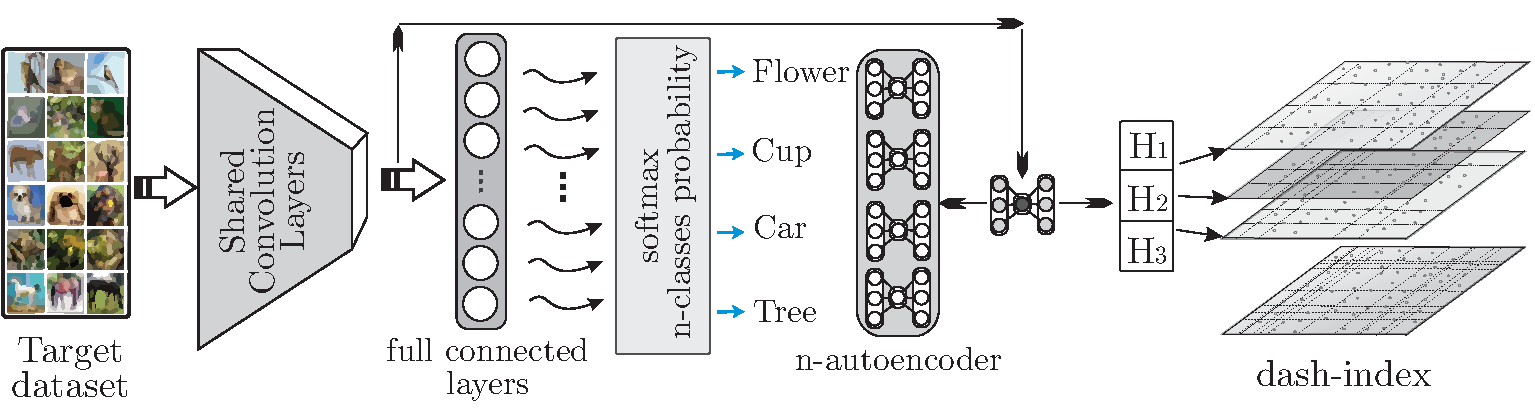
\includegraphics[width=1.0\columnwidth]{chapter6/DAsh_learning_final.pdf}
\caption{ DAsH. Proceso de entrenamiento e indexación. } 
\label{fig:dash}
\end{figure}    

Como se mostró en \cite{citeulike:fractal:encoders} un algoritmo de reducción de dimensionalidad exitoso proyecta los datos en un espacio de características con dimensionalidad cercana a la dimensionalidad fractal (FD) de los datos en el espacio original y conserva las propiedades topológicas.  Por lo tanto, para encontrar la dimensionalidad objetivo ($m$) que necesitan las redes de autoencodificadores seguimos la siguiente heurística.  Empezamos con el valor $m_1 = 2^2$, calculamos la FD del nuevo espacio con sólo eso, luego incrementamos el valor en $m_2 = 2^3$, recalculamos la FD, y continuamos haciendo esto hasta algún $ t\ (m_t =  2^t)$ donde podemos ver una mejora en la dimensión fractal, lo que significa que más características no cambian la dimensionalidad fractal del conjunto de datos.
 
El segundo paso de nuestro procedimiento es la recuperación de la imagen vía  DAsH. Procesamos la imagen de consulta enviándola a través de CNN con el objetivo de obtener las clases $n$ más fuertes. En contraste con los algoritmos de aprendizaje de similitud existentes que aprenden la similitud de la característica de bajo nivel, nuestra similitud es la combinación de similitud semántica y nivel de hashing. Así que, la similitud de nivel semántico se calcula en primer lugar. Después de la comprobación de relevancia semántica, obtendremos las nuevas consultas ($q_1, q_2, ... q_n$) usando los  $n$ autoencoders más fuertes. La consulta es transformada en una nueva consulta de objetos ($q_1, q_2, ... q_n$) los cuales son escogidos para localizar los apropiados \textit{buckets}. Una vez que los \textit{buckets} son localizados, el conjunto de candidatos relevantes son formados.  Luego, los elementos del conjunto candidato se analizan exhaustivamente con el fin de recuperar sólo los objetos que satisfacen la condición de consulta. Este proceso es realizado para cada una de las  $L$ tablas hash . Este proceso es ilustrado en la Figura \ref{fig:qdash}.  
\begin{figure}[htp]
\centering
 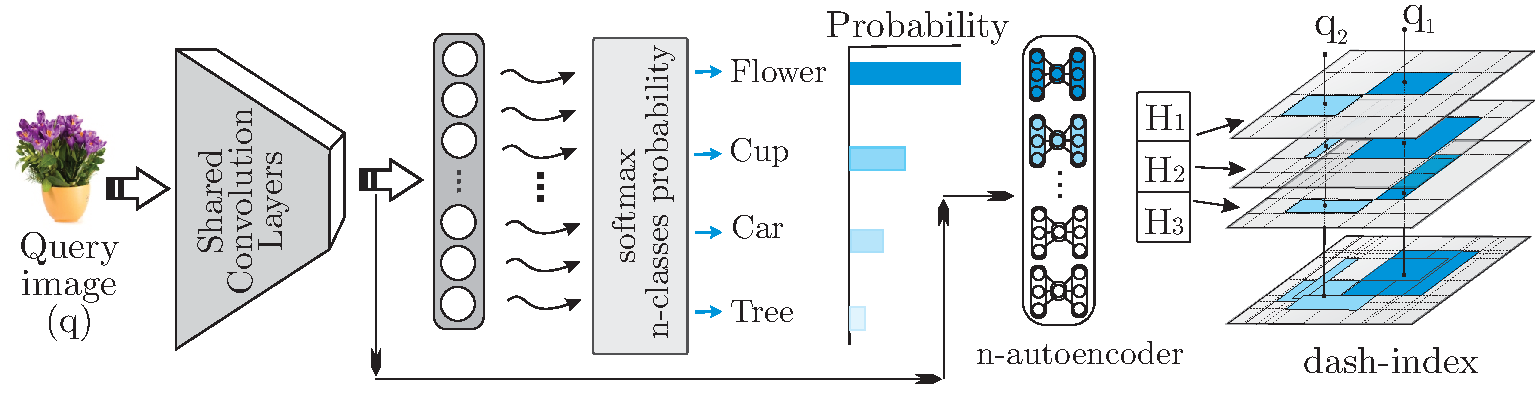
\includegraphics[width=1.00\columnwidth]{chapter6/DAsh_retrieval_final.pdf} 
 \caption{ DAsH. Proceso de recuperación. } 
\label{fig:qdash}
\end{figure} 
 
 \newpage

 \subsection{Usando la Dimensión Fractal para estimar los parámetros LSH}
 
 

Estamos interesados en averiguar la escala de resolución $log(r)$ en la que hay aproximadamente $k$ objetos. Recordando del Capítulo 4, la Ecuación \ref{eq:logpc_fractal} ($log(PC(r)) = \mathfrak{D} \times log (r) + K_p$) relaciona el número de pares $PC(r)$ a una distancia $r$, en base a estas   variables  debe ser posible calcular esta escala. Teniendo un subconjunto de elementos $k$ del conjunto de datos, el número de pares que generan estos elementos es el siguiente: 
 
\begin{equation}\label{eq:pairsk}
 Pairs(k) = k \cdot (k - 1) / 2 
\end {equation} 
 
\begin{figure}[htp]
\centering
 \includegraphics[width=0.650\columnwidth]{chapter6/computeKusingfractals.pdf} 
 \caption{ Cómo usar el Diagrama  de Distancia de un conjunto de datos para estimar el radio $r$ para una consulta  $kNN$. } 
\label{fig:knnfractal}
\end{figure} 
Dado un conjunto de datos con cardinalidad $N$, el número de pares separados por distancias menores al diámetro ($R$) del conjunto de datos  es $PC (R) = Pairs (N) = N \cdot (N-1) / 2 $. Por lo tanto, se puede encontrar una línea  para el conjunto de datos asociada al punto $ <log (R), log (Pairs (N))>$ en el Diagrama de Distancia del conjunto de datos.  Usando esta línea, el número de elementos $k$ que forman pares a una distancia menor o igual a $r$ se puede estimar usando $PC (r) = Pairs (k)$. 

 La Figura \ref{fig:knnfractal} ilustra esta idea. En esta figura, La 'Línea 0' es la línea utilizada para calcular la dimensión intrínseca $\mathfrak{D}$ del  conjunto de datos. Esta línea se aproxima al número promedio de puntos (en la escala logarítmica) en toda la gama de distancias que se producen en el conjunto de datos. Obsérvese que los conjuntos de datos reales suelen tener menos distancias con valores cercanos al diámetro del conjunto de datos, por lo que el conteo de las distancias más grandes aumenta a un ritmo más lento que el conteo de distancias medias o pequeñas. Esta es la razón del aplanamiento de las típicas gráficas de conteo de pares en un amplio radio de conjuntos de datos reales.
  
Considerando el  punto $<log (R), log (Pairs (N))>$, identificado  el Punto  0 en la Figura \ref{fig:knnfractal}, se puede calcular la constante $K_p$ de la Ecuación \ref{eq:logpc_fractal} de la 'Línea 1' como:

\begin{equation}\label{eq:fractal_kd}
  K_p    = log (Pairs(N)) - \mathfrak{D} \cdot log (R) 	
\end{equation}

Del mismo modo para el punto $<log (r), log (Pairs (k))>$  y combinando la Ecuación \ref{eq:pairsk} con la Ecuación \ref{eq:logpc_fractal} se obtiene:
  
\begin{equation}\label{eq:fractal_kd0}
  K_p = log (Pairs (k)) - \mathfrak{D} \times log (r)
\end{equation}

Luego, combinando la Ecuación \ref{eq:fractal_kd} con la Ecuación \ref{eq:fractal_kd0} se obtiene:

\begin{eqnarray}\label{eq:fractalR}
  log (Pairs(k)) - \mathfrak{D} \times log (r)) &=& log (Pairs(N)) - \mathfrak{D} \cdot log (R)   \nonumber \\
  \mathfrak{D} \cdot log (r) &=& log (Pairs (k)) - log (Pairs(N)) + D log (R)   \nonumber \\
  r &=& R \cdot  exp (  \frac{log (Pairs (k)) - log (Pairs(N))}{ \mathfrak{D} } )    
\end{eqnarray}

Entonces, la Ecuación \ref{eq:fractalR} permite estimar el radio $r$ para una consulta  $kNN$.  Usando la misma generalización podemos estimar  el número óptimo de funciones hash $m$ para un índice basado en \textit{LSH} configurado para recuperar los $k$ vecinos más cercanos. Podemos decir que $m$ es proporcional a $log ( Pairs(k) ) = log ( PC(r) )$ pues $log ( PC(r) )$ representa el nivel de correlación entre los datos a una escala de radio $r$. Esto tiene sentido, porque existen un promedio de $k$ vecinos  dentro de una distancia $r$. Entonces, definimos:
\begin{equation}\label{eq:optimalM1}
   m \approx log (PC(r)) 
\end{equation}

combinando las ecuaciones \ref{eq:optimalM1} y \ref{eq:fractal}  ($PC(r) = K_p \times r^{\mathfrak{D}}$). Simplificando obtenemos  que $m \approx \mathfrak{D} \cdot log (r)  $. Recordando que $r$ se puede calcular usando la Ecuación \ref{eq:fractalR}. Experimentalmente, confirmamos que el valor óptimo de $m$ es:

 \begin{equation}\label{eq:fractalm}
    m = (\left\lceil \mathfrak{D} + 1 \right\rceil  ) \cdot  log (r)
 \end{equation}
% Nivel de correlación a escala logaritmica en un radio r. 
 
\section{Experimentos}

En esta sección, estamos interesados en responder a la siguiente pregunta: (a) ¿Qué tan preciso es nuestro modelo en la estimación de los parámetros LSH utilizando la dimensión fractal?; (B) ¿Cómo mejora nuestro método DAsH las otras implementaciones de LSH en términos de \textit{consultas de rendimiento} y \textit{precisión}?. El rendimiento del método DAsH se comparó con los de los dos métodos más conocidos, llamado Multi-probe LSH \cite{multiprobe} y LSH-Forest \cite{lshforest}. Todos los experimentos se realizaron en un workstation con Intel core i7  3.0Ghz (12 núcleos) CPU y 64Gb de RAM con cuatro tarjetas gráficas Geforce GTX 1080 GPU de 8Gb VRAM cada una.
 
Primero realizamos experimentos en ocho conjuntos de datos ampliamente utilizados usando características hechas a mano (AUDIO, CITIES, EIGENFACES, HISTOGRAMS, MGCOUNTY, RANDOMWALK, SYNTH16D, SYNTH6D, VIDEO) \footnote{\url{https://github.com/joselhuillca/fractal_dataset}} para evaluar nuestro método propuesto para estimar los parámetros LSH. Además de las características hechas a mano, también mostramos la eficacia de nuestros métodos cuando las características son extraídas por las Redes Neuronales Convolucionales profundas (CNN), realizamos este experimento en tres conjuntos de datos (MNIST\footnote{\url{http://yann.lecun.com/exdb/mnist/}}, CIFAR-10\footnote{\url{https://www.cs.toronto.edu/~kriz/cifar.html}}, SVHN\footnote{\url{http://ufldl.stanford.edu/housenumbers/}}) para evaluarlos en términos de \textbf{consultas de rendimiento} y \textbf{mean average precision (mAP)}. A continuación se describen los detalles de los experimentos y resultados.

\subsection{Experimento 1: Sintonización de parámetros LSH}

Los métodos basados en LSH reportan resultados eficientes cuando los valores $m$ (número de funciones hash) son elegidos.Para evaluar la eficacia del enfoque presentado para afinar los parámetros LSH utilizando la dimensión fractal, hemos trabajado en una variedad de datos sintéticos y reales. Tabla \ref{table:lshparams} y la Figura \ref{fig:fractal-params} resume las principales características y parámetros de los conjuntos de datos, incluyendo el número de elementos $N$, el número de atributos $d$, su dimensión intrínseca (fractal) $D$ y los parámetros LSH usando dos aproximaciones: el algoritmo de Andoni \footnote{\url{http://www.mit.edu/~andoni/LSH/}}  y nuestra propuesta basada en dimension fractal.  os resultados del experimento para el número de funciones de hash $m$ muestran que las estimaciones dadas por la ecuación \ref{eq:fractalm} son comparables con las obtenidas con el algoritmo E2LSH propuesto por Andoni utilizando hasta 10 veces menos tiempo.
 
\begin{table}[!t]
\caption{Parámetros óptimos  de LSH usando el método de fuerza bruta $e2lsh$ y el método basado en dimension fractal.}
\label{table:lshparams}
\centering
\begin{footnotesize}
\begin{tabular}{c|r|r|r|r|r|r|r|r|r|r|}
    \cline{2-11}
    & \multicolumn{ 2}{|c|}{{\bf dataset}} & \multicolumn{ 3}{|c|}{{\bf fractal params}} & \multicolumn{ 2}{|c|}{{\bf e2lsh}} & \multicolumn{ 3}{|c|}{{\bf fractalsh}}  \\
    \cline{2-11}
    & \multicolumn{1}{c|}{$N$}    & \multicolumn{1}{c|}{$d$} & \multicolumn{1}{c|}{$\mathfrak{D}$}    & $log(R)$ & $log(PC(R))$   & $m$ & \multicolumn{1}{c|}{$time(s)$}    & \multicolumn{1}{c|}{$r$}  & $m$ & \multicolumn{1}{c|}{$time(s)$} \\
    \hline
\multicolumn{1}{|c|}{\bf audio}                 & 54387                 & 192      & 6.49     & -1.30      & 17.00       & \cellcolor[HTML]{f2f2f2}18                        & \cellcolor[HTML]{f2f2f2}64.20     & 0.14  & \cellcolor[HTML]{DFDFDF}16                    & \cellcolor[HTML]{DFDFDF}12.68                   \\
\multicolumn{1}{|c|}{\bf cities}                & 5507                  & 2        & 2.36     & 2.30       & 16.00       & \cellcolor[HTML]{f2f2f2}8                         & \cellcolor[HTML]{f2f2f2}16.45      & 4.16  & \cellcolor[HTML]{DFDFDF}6                     & \cellcolor[HTML]{DFDFDF}0.81                    \\
\multicolumn{1}{|c|}{\bf eigenfaces}            & 11900                 & 16       & 4.25     & -1.40      & 18.00       & \cellcolor[HTML]{f2f2f2}12                        & \cellcolor[HTML]{f2f2f2}42.28      & 0.13  & \cellcolor[HTML]{DFDFDF}13                    & \cellcolor[HTML]{DFDFDF}1.57                    \\
\multicolumn{1}{|c|}{\bf histograms}            & 4247                  & 256      & 2.50     & -0.81      & 16.01       & \cellcolor[HTML]{f2f2f2}6                         & \cellcolor[HTML]{f2f2f2}15.62      & 0.22  & \cellcolor[HTML]{DFDFDF}7                     & \cellcolor[HTML]{DFDFDF}6.12                    \\
\multicolumn{1}{|c|}{\bf mgcounty}              & 27282                 & 2        & 1.81     & 0.70       & 19.00       & \cellcolor[HTML]{f2f2f2}4                         & \cellcolor[HTML]{f2f2f2}87.96      & 0.27  & \cellcolor[HTML]{DFDFDF}4                     & \cellcolor[HTML]{DFDFDF}1.13                     \\
\multicolumn{1}{|c|}{\bf randomwalk}            & 10000                 & 1024     & 5.52     & 2.80       & 15.00       & \cellcolor[HTML]{f2f2f2}16                        & \cellcolor[HTML]{f2f2f2}50.60     & 10.16 & \cellcolor[HTML]{DFDFDF}17                    & \cellcolor[HTML]{DFDFDF}10.60                   \\
\multicolumn{1}{|c|}{\bf synth16d}              & 10000                 & 16       & 8.36     & -1.40      & 17.00       & \cellcolor[HTML]{f2f2f2}20                        & \cellcolor[HTML]{f2f2f2}27.20     & 0.18  & \cellcolor[HTML]{DFDFDF}18                    & \cellcolor[HTML]{DFDFDF}7.51                   \\
\multicolumn{1}{|c|}{\bf synth6d}               & 10000                 & 6        & 4.95     & -1.40      & 17.00       & \cellcolor[HTML]{f2f2f2}12                        & \cellcolor[HTML]{f2f2f2}28.16      & 0.14  & \cellcolor[HTML]{DFDFDF}12                    & \cellcolor[HTML]{DFDFDF}6.47                    \\
\multicolumn{1}{|c|}{\bf video}                 & 79094                 & 50       & 7.73     & -1.40      & 21.00       & \cellcolor[HTML]{f2f2f2}16                        & \cellcolor[HTML]{f2f2f2}1205.73     & 0.13  & \cellcolor[HTML]{DFDFDF}19                    & \cellcolor[HTML]{DFDFDF}92.54                   \\ 
\hline
\end{tabular}
\end{footnotesize}
\end{table}
%Gracias a esta relación entre los parámetros LSH y la dimensión fractal, podemos trabajar con datos a gran escala. Además, debido a la dimensión fractal se puede estimar en tiempo lineal podemos estimar óptimamente los parámetros de LSH en tiempo lineal también. 
\begin{figure}[htp]\centering
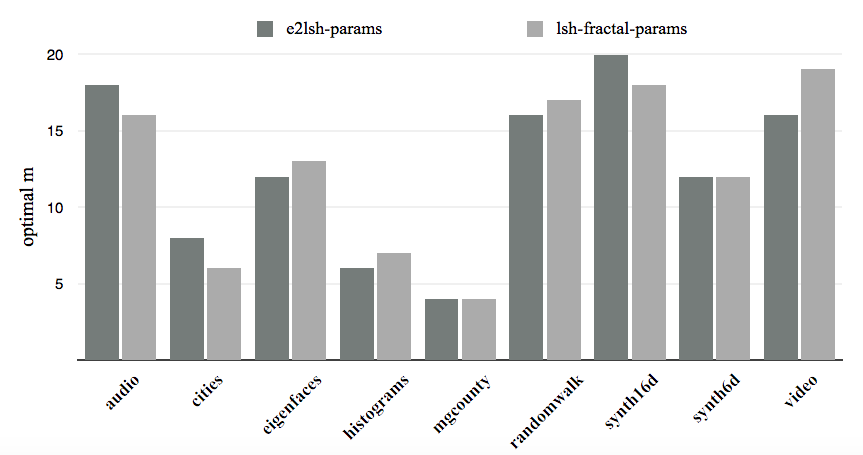
\includegraphics[width=0.9\columnwidth]{chapter6/fractal-params.png}
\caption{Comparación gráfica de los parámetros óptimos  de LSH usando el método de fuerza bruta $e2lsh$ y el método basado en dimension fractal.}
\label{fig:fractal-params}
\end{figure}    
\begin{table}[!htp]
\caption{Mean Average Precision(mAP), Precisión (P) y el tiempo acumulado invertido en el cálculo de mAP para diferentes métodos en los conjuntos de datos MNIST, SVHN y CIFAR-10. }
\label{table:map}
\centering
\begin{footnotesize}
\begin{tabular}{l|c|c|c|c|c|c|c|c|c|}
\cline{2-10}
                                           & \multicolumn{3}{c|}{\textbf{MNIST}}            & \multicolumn{3}{c|}{\textbf{SVHN}}             & \multicolumn{3}{c|}{\textbf{CIFAR-10}}         \\ \cline{2-10} 
                                           & \textbf{mAP} & \textbf{P (\%)} & \textbf{time(s)} & \textbf{mAP} & \textbf{P (\%)} & \textbf{time(s)} & \textbf{mAP} & \textbf{P (\%)} & \textbf{time(s)} \\ \hline
\multicolumn{1}{|l|}{\textbf{MpLSH  }}       & 0.86         & 0.95            & \cellcolor[HTML]{c8c8c8}19.58         & 0.71         & 0.73            & 8.09          & \cellcolor[HTML]{c8c8c8}0.83         & 0.89            & \cellcolor[HTML]{c8c8c8}122.45        \\ \hline
\multicolumn{1}{|l|}{\textbf{ITQ  }}         & 0.87         & 0.95            & 1297.32       & 0.70         & 0.80            & 8411.26       & 0.84         & 0.88            & 1056.83       \\ \hline
\multicolumn{1}{|l|}{\textbf{LOPQ  }}        & 0.86         & 0.90            & 119.21        & 0.71         & 0.74            & 613.65        & 0.83         & 0.88            & 528.20        \\ \hline
\multicolumn{1}{|l|}{\textbf{LSH-F  }}       & 0.85         & 0.96            & 217.33        & 0.61         & 0.78            & 365.90        & 0.86         & 0.89            & 365.47        \\ \hline
\multicolumn{1}{|l|}{\textbf{DAsH (Ours)}} & \cellcolor[HTML]{c8c8c8}0.93         & \cellcolor[HTML]{c8c8c8}0.98            & \cellcolor[HTML]{f2f2f2}20.82         & \cellcolor[HTML]{c8c8c8}0.74         & \cellcolor[HTML]{c8c8c8}0.84            & \cellcolor[HTML]{f2f2f2}10.34         & \cellcolor[HTML]{c8c8c8}0.88         & \cellcolor[HTML]{c8c8c8}0.91            & \cellcolor[HTML]{f2f2f2}125.37        \\ \hline
\end{tabular}
\end{footnotesize}
\end{table}
\subsection{Rendimiento de Recuperación} % OK
El objetivo de este experimento es medir el tiempo total dedicado a recuperar los objetos vecinos $k$-nearest. Las estructuras de datos que se compararon se probaron con valores específicos para las consultas. Por lo tanto, usamos $k = 1000$ cuando calculamos la métrica de Mean Average Precision ($mAP$) y $k = 25$ cuando calculamos la métrica de precisión $ (P(\%))$.

La Tabla  \ref{table:map} muestra la comparación en términos de mean average precision (mAP)  y tiempo de consulta para todos los métodos basados en hash. El método DAsH fue significativamente mejor que otros métodos; proporcionando hasta un mAP 10 \% mejor,  manteniendo un excelente tiempo de recuperación. Este resultado demuestra el potencial de impulsar las operaciones de consulta con el diseño de estructuras de índices especializados.
 


\bibliographystyle{plain}
\bibliography{references}
\appendix
\setcounter{chapter}{0}
\renewcommand{\chaptername}{Appendix}
%\renewcommand{\thechapter}{\arabic{section}.\arabic{ind}}
\renewcommand{\theequation}{\Alph{chapter}.\arabic{section}.\arabic{equation}}
\addcontentsline{toc}{chapter}{\numberline{}Appendix}
\setcounter{equation}{0}
\chapter{Basic and Auxiliary Results}
\section{Basic Results}



\end{document}
